\documentclass[acronym, symbols, table, deposito]{fei}

%\usepackage[xcdraw]{xcolor}
\usepackage{pgfplots}
\usetikzlibrary{pgfplots.statistics}
\pgfplotsset{compat=1.18}
\usepackage{pgfplotstable}

\usepackage{pdfpages}
\usepackage{float}
\usepackage{glossaries}
\usepackage{filecontents}
\usepackage{subcaption}
\usepackage{chngcntr}
\usepackage{float}
\usepackage[portuguese]{algorithm2e}
\usepackage{biblatex}
\usepackage{amsmath}

%\usepackage{algorithm}
%\usepackage{algpseudocode}
%\usepackage[utf8]{inputenc}
\usepackage{chngcntr} %Faz com que o numero das notas de rodape aumente crescentemente
\usepackage{appendix}
\usepackage{amsfonts}
\usepackage{graphicx, booktabs, caption, adjustbox, multicol}
\counterwithout{footnote}{chapter}% "

% escrita que precede cada entrada na lista de ilustrações
\renewcommand{\cftfigurepresnum}{Figura }
\setlength{\cftfigurenumwidth}{5.7em}

\title{Fusão de sensores para estimativa de localização de robôs no ambiente da RoboCup Small Size League}
\author{João Victor Lourenço Aguiar}
\cidade{São Bernardo do Campo}
\instituicao{Centro Universitário FEI}

\addbibresource{Referencias.bib}
%\bibliographystyle{plain}
\nocite{*}
\bibliography{Referencias.bib}
\graphicspath{ {Imagens/} }

\makeglossaries
\newacronym{kf}{KF}{Filtro de Kalman}
\newacronym{ekf}{EKF}{Filtro de Kalman Estendido}
\newacronym{ukf}{UKF}{Filtro de Kalman \textit{Unscented}}
\newacronym{kg}{KG}{Ganho de Kalman}
\newacronym{ssl}{SSL}{\textit{Small Size League}}
\newacronym{imu}{IMU}{\textit{Inertial Measurement Unit}}
\newacronym{tdp}{TDP}{\textit{Team Description Paper}}
\newacronym{afls}{AFLS}{Adaptative Fuzzy Logic System}
\newacronym{fp}{FP}{Filtro de Partículas}
\newacronym{dc}{DC}{\textit{Direct Current}}
\newacronym{mems}{MEMS}{Sistema Microeletromecânico}
\newacronym{ins}{INS}{\textit{Inertial Navigation System}}
\newacronym{msl}{MSL}{\textit{Middle Size League}}
\newacronym{fsev}{FSEV}{Filtro Suave de Estrutura Variável}
\newacronym{i2c}{I²C}{\textit{Inter-Integrated Circuit}}
\newacronym{spi}{SPI}{\textit{Serial Peripheral Interface}}
\newacronym{muv}{MUV}{Movimento Uniformemente Variado}
\newacronym{pcb}{PCB}{\textit{Printed Circuit Board}}

%\newglossaryentry{tensao}
%{
%	type=symbols,
%	name=$V$,
%	description=Tensão elétrica,
%	symbol=$V$
%}

\newglossaryentry{potencia}
{
	type=symbols,
	name=$W$,
	description=Potência,
	symbol=$W$
}
%
%\newglossaryentry{metros}
%{
%	type=symbols,
%	name=$m$,
%	description=Metros,
%	symbol=$m$
%}

\begin{document}
	
\maketitle

\begin{folhaderosto}
	Dissertação de Mestrado apresentada ao Centro Universitário da FEI para obtenção do título de Mestre em Engenharia Elétrica, orientado pelo Prof. Dr. Flavio Tonidandel.
\end{folhaderosto}

\fichacatalografica

\begin{agradecimentos}
	Eu gostaria de agradecer à minha família, especialmente pais e irmão, por todo apoio durante a jornada e pelo suporte para que eu pudesse focar nos estudos.
	
	Aos meus amigos, que também me apoiaram e motivaram durante essa etapa.
	
	Ao meu orientador, Prof. Dr. Flavio Tonidandel, que me ajudou desde o começo da graduação quando ingressei no projeto RoboFEI e me ajudou a solucionar dúvidas, realizar discussões e providenciando orientações ao longo do caminho.
	
	A todos os membros da equipe SSL do RoboFEI que convivi durante esse tempo, além dos professores Plinio Thomaz Aquino Junior e Reinaldo Bianchi. Obtive muito conhecimento convivendo com todos no dia-a-dia e durante as competições que participei.
	
	O presente trabalho foi realizado com apoio da Coordenação de Aperfeiçoamento de Pessoal de Nível Superior - Brasil (CAPES) - Código de Financiamento 001.
\end{agradecimentos}

\begin{epigrafe}
	\epig{Aqueles que se sentem satisfeitos sentam-se e nada fazem. Os insatisfeitos são os únicos benfeitores do mundo.}{Walter Savage Landor}
\end{epigrafe}
	
\begin{resumo}
	
%	Este projeto propõe o estudo de sistemas de localização para robôs móveis utilizando filtro de Kalman. A fim de alcançar isso, diferentes sensores serão combinados e comparados para predição e correção da posição do robô, que no caso são: \textit{encoders} acoplados aos eixos dos motores utilizados para movimentação, \glsxtrshort{imu}, que é composta por um giroscópio e um acelerômetro, além do sistema de câmeras utilizado nas partidas da categoria \glsxtrshort{ssl}, que dispõe a posição e orientação dos robôs em campo. As combinações serão testadas no cenário de futebol de robôs da categoria \glsxtrshort{ssl}, que possui uma dinamicidade por conta da velocidade dos robôs e da bolinha em campo. Os resultados parciais alcançados são resumidos à obtenção dos dados dos sensores descritos, além da implementação dos cálculos do filtro de Kalman de forma embarcada no robô. A partir dos testes propostos espera-se investigar os pontos positivos e negativos das diferentes combinações a fim de identificar a melhor delas e alcançar um sistema de localização robusto que funciona de maneira embarcada.

%	Este projeto propõe o desenvolvimento de um sistema de localização para robôs móveis robôs da categoria \textit{Small Size} da RoboCup de futebol de robôs, a fim de melhorar seu posicionamento ao realizarem jogadas e diminuir a dependência do sistema de câmeras disponibilizados pela liga durante os jogos da categoria. O sistema de localização utiliza um filtro de Kalman para realizar a fusão de sensores, que no caso serão os \textit{encoders} acoplados aos eixos dos motores utilizados para movimentação dos robôs, uma \acrshort{imu}, composta por um giroscópio e um acelerômetro, ambos disponíveis no hardware dos robôs, além do sistema de câmeras da categoria que dispõe a posição e orientação dos robôs e bolinha em campo. Os resultados parciais são resumidos à obtenção dos dados dos diferentes sensores, além da implementação dos cálculos do filtro de Kalman no microcontrolador do robô. A partir dos testes propostos espera-se investigar os pontos positivos e negativos das diferentes combinações a fim de identificar a melhor delas e alcançar um sistema de localização robusto que funciona de maneira embarcada.

Este trabalho propõe o estudo de sensores para localização de robôs móveis no ambiente de futebol de robôs da categoria \acrlong{ssl} (\acrshort{ssl}) da RoboCup. Para isso, foram comparadas diferentes combinações de sensores, sendo eles: encoders acoplados aos eixos das rodas, sensor \glsxtrlong{imu} (\glsxtrshort{imu}) composto por giroscópio e acelerômetro, e câmeras externas pertencentes ao sistema compartilhado de visão da liga (SSL-Vision). O sistema é baseado em fusão de sensores, utilizando o \glsxtrshort{ekf} (Extended Kalman Filter). A seleção dos sensores baseou-se em uma análise dos trabalhos recentes desenvolvidos na categoria \acrshort{ssl}, identificando os sensores mais utilizados pelas equipes de ponta. Os sensores escolhidos foram testados utilizando um robô real da equipe RoboFEI, em dois cenários diferentes no campo de testes da equipe. O primeiro, localizado na região central do campo, sofre com sobreposição de câmeras e consequente duplicação de leituras. O segundo, de maiores dimensões e localizado nas bordas do campo, é afetado por distorções causadas pelas lentes olho de peixe. Para a avaliação, foram utilizadas duas métricas: o erro médio de distância em relação a um sistema de \textit{ground truth} e o tempo de atualização das estimativas de posição. Os sensores foram combinados dois a dois entre as fases de predição e correção do \glsxtrshort{ekf}. O sistema de \textit{ground truth} foi desenvolvido especificamente para este trabalho, utilizando dois LiDARs externos ao robô e a transformada de Hough para identificação do padrão circular de um típico robô da categoria \acrshort{ssl} em uma imagem gerada com os pontos dos LiDARs. No primeiro teste, foi possível observar que as melhores combinações, em termos de erro médio de distância, utilizavam os dados do SSL-Vision na fase de correção, enquanto na fase de predição usavam leituras de sensores em vez do modelo cinemático do robô omnidirecional, evidenciando que os dados de sensores ajudam a estimar melhor a posição do robô. Quanto ao tempo de atualização, como os cálculos do \acrshort{ekf} para fusão de sensores são realizados de forma embarcada no microcontrolador do robô, notou-se que a fusão de sensores é cinco vezes mais rápida do que o sistema atualmente utilizado pela equipe. No segundo teste, foi notável que, nas combinações sem o SSL-Vision, tanto o erro médio de distância quanto os valores máximos aumentaram em relação ao primeiro teste. Isso evidencia um aumento do erro em trajetos maiores, além da necessidade de utilização de um sensor que forneça observações absolutas do robô dentro do ambiente. Por fim, com este trabalho foi possível realizar a comparação da utilização de diferentes sensores no ambiente de futebol de robôs, em um sistema de fusão de sensores para localização utilizando o \glsxtrshort{ekf} de forma embarcada. Conclui-se que, para a liga \glsxtrshort{ssl}, a utilização dos dados do SSL-Vision é inevitável para a correção da posição do robô, devido à precisão necessária na realização das jogadas durante a partida. No entanto, ao fundir sensores como \glsxtrshort{imu} e encoders aos dados das câmeras, foi possível obter estimativas de posição ligeiramente melhores, com tempos de atualização significativamente menores.
	
	\keywords{Localização. Predição. Correção. Sensores. Embarcado.}

\end{resumo}

\begin{abstract}
	
%	This project proposes studying localization systems for mobile robots using a Kalman Filter. Different sensors will be combined and compared to predict and correct the robot's pose to achieve that, namely: encoders attached to the motors' shafts used for movement, IMU composed of a gyroscope and an accelerometer, and the camera system used in the \glsxtrshort{ssl} games, that gives the pose and orientation of the robots in the field. The robot soccer of the \glsxtrshort{ssl} category will be the test scenario for these combinations. Partial results are summarized to obtain data from the sensors described, besides developing the code of the Kalman Filter calculations embedded in the robot. The strengths and weaknesses of each combination will be investigated given the tests proposed to choose the best of them and achieve a robust and embedded localization system.
	
%	This project proposes developing a localization system for the robots of the Small Size League from RoboCup to enhance their positioning while performing plays and decrease their dependence on the global system used in league games. The localization system uses a Kalman Filter to fuse different sensors, in this case, encoders attached to the motors' shafts used to move the robot, a gyroscope, and an accelerometer, both available on the robot's hardware, besides the cameras system used by the league that gives the poses and orientations of the robots and the ball in the field. Partial results are summarized to obtain data from the different sensors used in the project, besides developing the code of the Kalman Filter calculations embedded in the robot. The strengths and weaknesses of each combination will be investigated given the tests proposed to choose the best of them and achieve a robust and embedded localization system.

	This work proposes the study of sensors for mobile robot localization in the robot soccer environment of the \acrlong{ssl} (\acrshort{ssl}) category of RoboCup. To this end, different combinations of sensors were compared, namely: encoders attached to the wheel shafts, an \glsxtrlong{imu} (\glsxtrshort{imu}) sensor composed of a gyroscope and an accelerometer, and external cameras that are part of the league’s shared vision system (SSL-Vision). The system is based on sensor fusion using the Extended Kalman Filter (\glsxtrshort{ekf}). The selection of sensors was based on an analysis of recent works developed in the \acrshort{ssl} category, identifying the most commonly used sensors by top-performing teams. The selected sensors were tested using a real robot from the RoboFEI team in two different scenarios on the team's test field. The first scenario, located in the central region of the field, is affected by overlapping cameras, which causes position divergence due to duplicated readings. The second scenario, with larger dimensions and located near the edges of the field, is influenced by distortions caused by fisheye lenses. Two metrics were used for the evaluation: the average distance error relative to a ground truth system and the update time of position estimates. The sensors were combined in pairs between the prediction and correction phases of the \glsxtrshort{ekf}. The ground truth system was specifically developed for this work, using two LiDARs external to the robot and the Hough transform to identify the circular pattern of a typical \acrshort{ssl} robot in an image generated from the LiDAR point cloud. In the first test, it was observed that the best combinations in terms of average distance error used SSL-Vision data during the correction phase, while using sensor readings—rather than the kinematic model of the omnidirectional robot—in the prediction phase, highlighting that sensor data helps provide better position estimates. Regarding update time, since the \acrshort{ekf} calculations for sensor fusion are executed onboard the robot’s microcontroller, it was found that the fusion process is five times faster than the system currently used by the team. In the second test, it was notable that combinations without SSL-Vision showed increases in both average distance error and maximum error values compared to the first test. This indicates a rise in error over longer trajectories, as well as the need for a sensor capable of providing absolute observations of the robot within the environment. Finally, this work enabled a comparison of different sensors within the robot soccer environment, in a sensor fusion system for localization using an embedded \glsxtrshort{ekf}. It was concluded that, for the \glsxtrshort{ssl} league, the use of SSL-Vision data is essential for correcting the robot’s position due to the level of precision required for executing plays during a match. However, by fusing sensors such as \glsxtrshort{imu} and encoders, it was possible to achieve slightly better position estimates with significantly lower update times.
	
	
	
	\keywords{Localization. Prediction. Correction. Sensors. Embedded.}
	
\end{abstract}

\listoffigures
\listoftables
\listofalgorithms
%\printglossaries
\printglossary[type=\acronymtype]
\tableofcontents
\setcounter{table}{0}

\chapter{Introdução}

	A utilização de robôs móveis cresce cada vez mais em diferentes áreas da sociedade, como medicina, agricultura, serviços e indústrias de diferentes tipos, como química, automotiva, metalúrgica, alimentícia, entre outras. De acordo com \textcite{robotics_market}, a indústria global de robótica ultrapassou 37 bilhões de dólares e, se mantida a projeção de crescimento de 3,8\% ao ano, até o final de 2028 alcançará o valor de 45 bilhões de dólares, mostrando o crescimento da utilização dos robôs em diversos setores do mercado.
	
	Apesar de os robôs estarem sendo amplamente utilizados na indústria, eles também podem ser encontrados no dia-a-dia do ser humano cada vez mais, como robôs que limpam o chão de casa, que estão cada vez mais acessíveis. Além disso, pode-se citar o desenvolvimento e pesquisa de outras categorias de robôs, como sistemas de entrega por meio de drones \cite{su14010360} e carros autônomos \cite{parekh2022review}
	
	A característica que difere os robôs móveis dos robôs industriais, como os robôs manipuladores utilizados para montagem de carros na indústria automotiva, é a capacidade de navegação, que acaba sendo um problema desafiador para os robôs móveis. A navegação pode ser dividida em 4 subsistemas basicamente, que são: mapeamento, localização, planejamento e desvio de obstáculos \cite{app12146951}. 
	
	No caso desse projeto, a questão principal é a localização, que é responsável por determinar a posição e orientação do robô no ambiente. Dentro do escopo da localização, os principais pontos são o posicionamento/localização global e o rastreio da posição de robôs móveis dentro de um mapa conhecido.
	
	De acordo com \textcite{PANIGRAHI20226019}, o objetivo do rastreio da posição é acompanhar o posicionamento do robô a cada instante de tempo sabendo sua posição inicial, o que é possível monitorando continuamente a rota do robô, seja por meio de sensores ou das equações cinemáticas que descrevem o robô. Já na localização global, a localização inicial não é conhecida e, assim, o robô deve se localizar dentro do ambiente global.
	
%	Tomando como exemplo a odometria, um robô acompanha seu trajeto utilizando os dados odométricos enquanto navega em um ambiente conhecido. Entretanto, a incerteza ao longo do tempo da odometria confunde o robô sobre sua posição atual. Então, para a localização global é utilizado um outro sensor, como um laser ou câmera. Assim, as informações de ambos são combinadas para localizar o robô. Apesar da leitura de um sensor externo, a posição exata não pode ser diretamente medida pelo robô, ele pode apenas extrair dados do sensores para conseguir conhecimento sobre a melhor estimativa da sua localização.
	
	Basicamente, também segundo \textcite{PANIGRAHI20226019}, a localização pode ser dividida em duas etapas: a predição e a percepção. Na etapa de predição o robô faz o rastreio da posição utilizando sensores proprioceptivos, que medem informações do próprio robô e são atualizados numa alta frequência geralmente, para estimar sua posição. Entretanto, por conta do aumento da incerteza ao longo do tempo desse tipo de sensores, para a localização global é necessário que o robô corrija na etapa de percepção utilizando seus sensores exteroceptivos, que medem informações do robô em relação ao ambiente e são atualizados numa frequência baixa.
	
	Para unir os dados desses diferentes sensores é utilizada uma técnica conhecida como fusão de sensores, cuja ideia geral é unir dados de diferentes sensores levando a uma análise mais profunda e complexa de uma situação, o que não seria possível utilizando esses dados separadamente e/ou de maneira singular \cite{s16101569}. Assim, ao realizar a fusão dos dados de diferentes sensores, os pontos negativos de um sensor são minimizados por haver um outro sensor atuando nesse ponto fraco.
	
	Um ambiente que possui a característica de um sensor externo com uma taxa de latência alta, onde os robôs precisam se posicionar com uma ótima precisão e navegam de maneira rápida e dinâmica dentro do ambiente, é o futebol de robôs da categoria \textit{Small Size League} (\glsxtrshort{ssl}) da \textit{RoboCup}. Por conta disso, a escolha dos sensores a serem utilizados, análises, testes e conclusões estão relacionadas com este ambiente. Basicamente, é importante que os robôs tenham um alto controle do seu posicionamento para que possam realizar jogadas e que não causem colisões com outros robôs, além de que na liga há um sistema central de visão por meio de câmeras que rodam a 60 frames por segundo (fps).
	
	Embora a taxa de atualização do sistema de câmeras global da liga tenha uma taxa de atualização de aproximadamente 60fps, o que aparenta ser suficiente, a dinamicidade em que os jogos ocorrem na \glsxtrshort{ssl}, com a bola podendo chegar a uma velocidade de 6.5$m/s$, implica numa alta necessidade de que as habilidades do robô estejam embarcadas no seu processador, tais como a navegação, controle de posição e, por conta disso, a localização. Assim, com a alta taxa de atualização do processador, os robôs têm acesso às informações dos seus diversos sensores de maneira quase instantânea, o que aumenta a performance deles durante uma partida \cite{ubc_thunderbots_2015}.

%	A categoria \textit{Small Size} de futebol de robôs da \textit{RoboCup} tem uma característica muito dinâmica por conta da velocidade da bola utilizada, que pode chegar a até 6,5 m/s devido a limitações impostas nas regras da categoria, fazendo com que os passes e chutes sejam muito rápidos \cite{rules}. Sabendo disso, para a realização das jogadas que o software propõe e ser capaz de acompanhar esse dinamismo, faz-se necessário que os robôs tenham um sistema de controle de posição confiável e efetivo.
%	
%	O sistema de controle atual é realizado a partir da imagem de câmeras posicionadas acima do campo. Elas detectam os padrões de cores posicionados em cima dos robôs e, assim, identificam sua posição em campo e o número do robô em questão. É possível ver na Figura \ref{fig:color_patterns} os 16 números diferentes formados pelo padrão de cor que deve ser colocado em cima dos robôs para sua identificação pelo sistema de câmeras.
	
%	\begin{figure}[!htb]
%		\centering
%		\caption{Padrões de cores para identificação dos robôs.} 
%		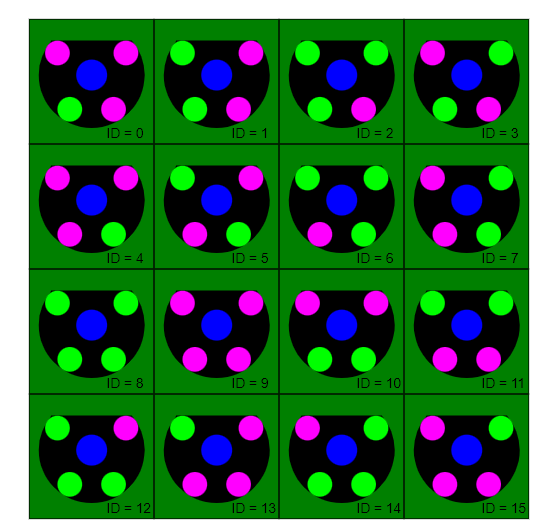
\includegraphics[width=0.5\textwidth]{Padrao_de_cores.eps}
%		\label{fig:color_patterns}
%		\smallcaption{Fonte: \textcite{rules}}
%	\end{figure}

%	As câmeras captam as imagens, enviam-nas para um computador que faz a identificação dos robôs e as transmitem para os times pela rede as posições dos robôs e seus IDs. A partir disso, o software atual da equipe RoboFEI faz o controle de posição junto a estratégia. 
%	
	
	\section{OBJETIVO}
	
		Este trabalho tem como objetivo realizar uma análise comparativa do uso de diferentes sensores para resolver o problema de localização e posicionamento de robôs móveis. No caso, os sensores a serem comparados foram a \textit{Inertial Measurement Unit} (\glsxtrshort{imu}), que é composta por um giroscópio e um acelerômetro, \textit{encoders} acoplados às rodas do robô, o sistema de câmeras utilizado na categoria \glsxtrshort{ssl} e, por fim, o modelo cinemático de um robô omnidirecional. Com essas combinações é possível verificar as diferenças da utilização desses sensores para um sistema de localização.
	
%		Este estudo tem como objetivo desenvolver um novo sistema de controle de posição para os robôs da categoria \textit{Small Size} da equipe RoboFEI que não seja tão dependente do sistema de câmeras utilizado durante as partidas da categoria. 
%		
%		Espera-se que o sistema desenvolvido possua uma latência de atualização menor, seja mais confiável e estável do que as câmeras em si. Assim, o time não seria dependente do sistema de visão externo fornecido pela liga e teria mais controle sob a questão do posicionamento dos robôs em si.
%		
%		Logo, este projeto irá investigar a utilização de sensores embarcados, tais como giroscópio, acelerômetro, \textit{encoders} e as próprias câmeras visando solucionar o problema de posicionamento de robôs móveis da categoria SSL da RoboCup.
%		
%		Após a implementação do novo sistema de controle de posição com a utilização de outros sensores, espera-se que com o problema de posicionamento sendo superado a equipe possa realizar as jogadas durante a partida com maior êxito, além de diminuir a quantidade de choque entre os robôs, ou seja, aumentando a qualidade de jogo da equipe.
		
	\section{JUSTIFICATIVA}
	
		De acordo com \textcite{alatise2020review}, a navegação é um problema fundamental para a robótica que acaba dependendo de outros aspectos para o seu bom funcionamento, como a localização. A tarefa de localização de robôs móveis em um ambiente arbitrário é um desafio por conta da complexidade e diversidade de ambientes, métodos e sensores envolvidos. Além disso, os problemas de localização e navegação são o que acabam limitando a performance de robôs ainda.
		
		Além disso, analisando trabalhos desenvolvidos na Small Size League que citam a questão da fusão de sensores \cite{Ryll2013TIGERSM, ubc_thunderbots_2017, parsian_2015, parsian_2019, mrl_2020, ubc_thunderbots_2015, immortals_2023}, é possível notar a falta de trabalhos que façam as devidas comparações entre os diferentes sensores usualmente utilizados num robô da \glsxtrshort{ssl}, além de trabalhos que comparem os resultados obtidos por um sistema de localização baseado em fusão de sensores com o sistema global de câmeras da categoria.
		
		Portanto, é importante que os diferentes sensores amplamente utilizados na categoria \glsxtrshort{ssl} para localização dos robôs e estimativa de posição sejam testados em um ambiente dinâmico, a fim de determinar os pontos fracos de cada um, formas de superar esses déficits e garantir o funcionamento deles de forma adequada em outros ambientes posteriormente.
	
	\section{Estrutura da dissertação}
	
		No Capítulo \ref{sec:chapter_futebol_robos} é feito o estudo do referencial teórico do futebol de robôs, onde os robôs da categoria \glsxtrshort{ssl} são descritos, os sensores a serem utilizados no trabalho e como estes devem ser calibrados. Já no Capítulo \ref{sec:chapter_localizacao_robos_moveis} são trazidos os conceitos necessários para entendimento do problema da localização de robôs móveis, com a explicação do método de fusão de sensores, além dos algoritmos para realização do método. No Capítulo \ref{sec:trab_relacionados} são apresentados os trabalhos relacionados, onde foram analisados os trabalhos correlatos que buscam resolver o problema da localização de robôs móveis, ou a estimativa de posição, mas também guiaram a escolha dos sensores, por exemplo, desse trabalho. No Capítulo \ref{sec:metodologia} é apresentada a metodologia deste trabalho, onde estão descritos os testes, o domínio onde os testes foram performados e como foram avaliados os dados retirados dos testes. O Capítulo \ref{sec:resultados} traz os resultados obtidos no projeto, desde a implementação do sistema de \textit{ground truth} desenvolvido, assim como a implementação dos cenários de fusão de sensores e os dados obtidos nos dois cenários de testes realizados. Por fim, o Capítulo \ref{sec:conclusao} traz a conclusão do projeto e os possíveis trabalhos futuros. % Já no Capítulo \ref{sec:resultados_parciais} são apresentados os resultados parciais conseguidos até o momento da banca de qualificação deste projeto. O cronograma dos dois anos de projeto é apresentado no Capítulo \ref{sec:cronograma}. O Capítulo \ref{sec:chapter_consideracoes_finais} traz as considerações finais e expectativas dos resultados para a continuação do projeto.
		
	\section{Contribuições}
	
		Nesta seção serão destacadas as contribuições desta dissertação.
		
		\subsection{Publicações}
		
			Os resultados obtidos para obtenção do ground truth do robô durante os testes foram publicados no 1º Congresso Brasileiro de Robótica. No artigo foram apresentados os conceitos utilizados para o desenvolvimento do sistema, assim como os resultados obtidos comparado com o sistema de visão utilizado na categoria \glsxtrshort{ssl}.
			
			A publicação também contou com uma apresentação de 15 minutos no simpósio.
			
		\subsection{Materiais eletrônicos}
		
			O repositório com os códigos do firmware\footnote{\href{https://github.com/JoaoVictor0508/object_detetection/tree/main}{github.com/JoaoVictor0508/object\_detetection}} utilizado ao longo dos testes, assim como do sistema de \textit{ground truth}\footnote{\href{https://github.com/JoaoVictor0508/firmware_ssl}{github.com/JoaoVictor0508/firmware\_ssl}} desenvolvido para esse projeto, foram disponibilizados para análise do desenvolvimento do projeto e para consulta em possíveis trabalhos futuros.

	\chapter{Futebol de robôs}\label{sec:chapter_futebol_robos}
	
		A ideia de robôs que jogam futebol foi proposta pela primeira vez pelo professor Alan Mackworth, em seu artigo \textit{On Seeing Robots} \cite{OnSeeingRobots}. Independentemente, em outubro de 1992, um grupo de pesquisadores japoneses organizou um workshop sobre os grandes desafios em IA, onde iniciaram-se as primeiras discussões sobre usar o futebol para promoção da ciência e tecnologia. Em junho de 1993 foi organizada uma competição de robótica e, em menos de um mês, pesquisadores de fora do Japão começaram a pedir que essa iniciativa fosse ampliada para um projeto conjunto internacional. Com isso foi criada a RoboCup em 1997 \cite{RoboCup}
		
		A \textit{RoboCup} busca promover pesquisas na área de robótica e inteligência artificial com um objetivo final de vencer a seleção campeã do mundo em 2050 com uma equipe totalmente autônoma de robôs humanoides \cite{RoboCup}.
		
		O atual cenário competitivo da \textit{RoboCup} mostra equipes tanto do ensino superior quanto do ensino básico que disputam diversas categorias, em eventos tanto a nível nacional quanto a nível internacional, tais como \textit{RoboCup Soccer}, \textit{RoboCup Rescue}, \textit{RoboCup@home} e a \textit{RoboCup Junior}.
	
	\section{\textit{Small Size League}} \label{sec:small_size_league}
	
		A \textit{Small Size League} (SSL) é uma das ligas mais antigas da \textit{RoboCup Soccer}, tendo o foco em solucionar o problema da cooperação e controle de robôs inteligentes num ambiente altamente dinâmico com um sistema híbrido centralizado/distribuído. A partida ocorre entre duas equipes utilizando seis ou onze robôs totalmente autônomos, que tem um limite de diâmetro e altura, e algumas outras restrições \cite{RoboCup}. Além disso, os robôs da liga são omnidirecionais, o que proporciona jogos dinâmicos com jogadas imprevisíveis.
		
		Os jogos desta categoria são destacados por conta da alta velocidade tanto dos robôs, que podem chegar até 4m/s, quanto da bola utilizada, que pode chegar até 6.5m/s, mas também pela quantidade de robôs numa partida, que acontece entre dois times que podem ter de 6 a 11 robôs num campo de 9m X 6m a 12m X 9m, dependendo da divisão da partida \cite{rules}.
		
		O tamanho do campo em relação aos robôs, a quantidade de robôs em uma partida e as velocidades dos robôs e da bolinha são algumas características que tornam a \glsxtrshort{ssl} um ótimo lugar para testes de algoritmos de localização e posicionamento.
		
		Para realização da partida, um \textit{setup} específico é necessário. No caso, acima do campo são instaladas câmeras, as imagens delas são processadas em um computador central que disponibiliza, a partir de pacotes de rede, as posições $x$ e $y$ e a orientação $\theta$ dos robôs em campo, além das posições $x$ e $y$ da bola, como ilustrado na Figura \ref{fig:ilustracao_partida_ssl}. O processamento das imagens e cálculo das posições são realizados por um sistema desenvolvido pela própria liga, chamado de SSL-Vision \cite{10.1007/978-3-642-11876-0_37}.
		
		\begin{figure}[!htb]
			\centering
			\caption{Ilustração de uma partida da \acrshort{ssl}.} 
			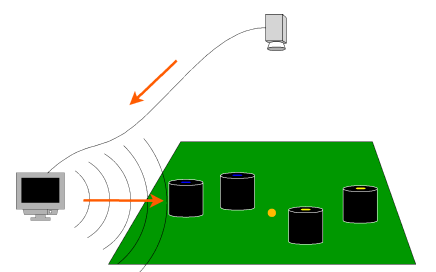
\includegraphics[width=0.5\textwidth]{funcionamento_ssl.png}
			\label{fig:ilustracao_partida_ssl}
			\smallcaption{Fonte: Retirado de \textcite{about-ssl}}
		\end{figure}
		
		Além disso, os robôs possuem limitações de tamanho, i.e., eles devem caber num diâmetro de 180mm e possuir uma altura máxima de 150mm \cite{rules}. A fim de lidar com essa limitação de dimensões e possuir robôs ágeis, as equipes utilizam um sistema de deslocamento omnidirecional, que é conseguido utilizando uma adaptação de rodas mecanum, em que os roletes são montados com uma certa angulação em relação ao eixo da roda \cite{aguiarreformulaccao}.
		
		Com esse sistema de deslocamento omnidirecional, o robô torna-se um sistema holonômico, i.e., o robô possui controle sobre todos os graus de liberdade da sua movimentação, ou seja, a rotação dele não interfere na translação, o que torna a \acrshort{ssl} uma liga muito dinâmica e imprevisível. A Figura \ref{fig:exemplo_robo_ssl} mostra um robô \acrshort{ssl} da equipe RoboFEI, nela é possível observar a roda omnidirecional utilizada.
		
		\begin{figure}[!htb]
			\centering
			\caption{Imagem de um robô \acrshort{ssl} da equipe RoboFEI.} 
			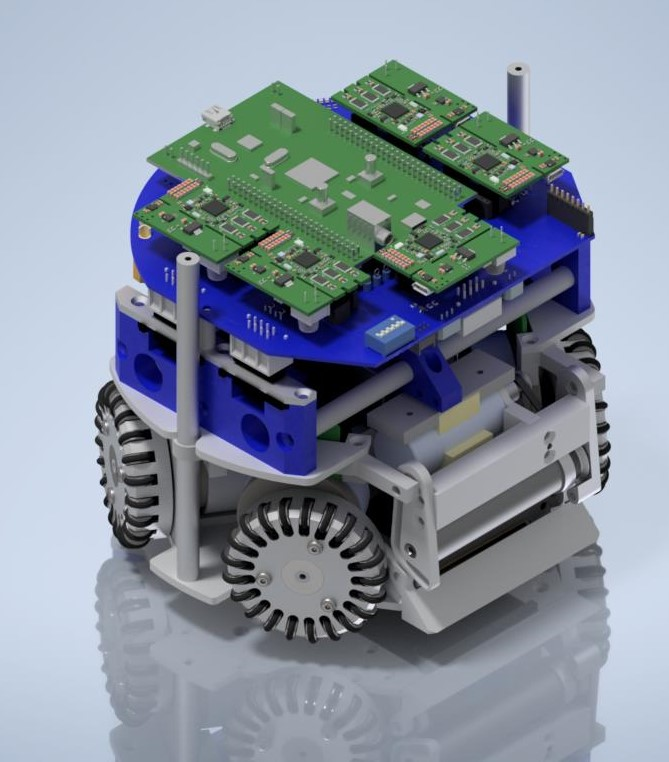
\includegraphics[width=0.4\textwidth]{Foto_Robo_2012.jpg}
			\label{fig:exemplo_robo_ssl}
			\smallcaption{Fonte: Autor}
		\end{figure}
		
		No caso, a Equação \eqref{eq:modelo_sistema_ssl} descreve as equações cinemáticas de um robô da categoria \glsxtrshort{ssl}, isto é, como teoricamente a posição de um robô propaga ao longo do tempo a partir de comandos de velocidade. As variáveis $x_k$, $y_k$ e $\theta_k$ representam as posições linear e angular do robô no instante atual $k$, enquanto $Vx_{k-1}$, $Vy_{k-1}$ e $\omega_{k-1}$ representam as velocidades linear e angular enviadas ao robô no instante de tempo anterior.
		
		\begin{equation}\label{eq:modelo_sistema_ssl}
			\begin{bmatrix}
				x_k \\
				y_k \\
				\theta_k
			\end{bmatrix} = 
			\begin{bmatrix}
				1 & 0 & 0 \\
				0 & 1 & 0 \\
				0 & 0 & 1
			\end{bmatrix} \times
			\begin{bmatrix}
				x_{k-1} \\
				y_{k-1} \\
				\theta_{k-1}
			\end{bmatrix} + 
			\begin{bmatrix}
				dt & 0 & 0 \\
				0 & dt & 0 \\
				0 & 0 & dt
			\end{bmatrix} \times
			\begin{bmatrix}
				Vx_{k-1} \\
				Vy_{k-1} \\
				\omega_{k-1}
			\end{bmatrix}
		\end{equation}
		
		Já o sistema de visão global da categoria \glsxtrshort{ssl}, que faz a captura de todos os robôs em campo e da bola, pode ser caracterizado conforme a Equação \eqref{eq:modelo_visao_ssl}, em que $\textbf{z}_{k}$ representa o vetor de medições do SSL-Vision no instante $k$. É possível notar que a visão fornece diretamente a posição do robô acrescida de um certo ruído $\sigma$.
		
		\begin{equation}\label{eq:modelo_visao_ssl}
			\textbf{z}_k  = 
			\begin{bmatrix}
				x_k \\
				y_k \\
				\theta_k
			\end{bmatrix} \pm
			\begin{bmatrix}
				\sigma_x \\
				\sigma_y \\
				\sigma_{\theta}
			\end{bmatrix}
		\end{equation}
		
		\subsection{Sistema de visão da categoria \glsxtrshort{ssl}}
		
			Durante a partida o processamento da tomada de decisões é feito num computador central de cada equipe, analisando as posições dos robôs e da bolinha em campo e, assim, enviando por meio de rádio frequência o que cada robô deve realizar, tal como: a velocidade de cada robô, se o robô deve chutar, se o robô deve ligar o dispositivo de drible, entre outros. Atualmente, na equipe RoboFEI, o cálculo do controle de posicionamento dos robôs é feito junto ao código da equipe e somente a velocidade angular e linear que o robô deve impor é passado para ele no pacote de dados via rádio.
		
			Apesar do sistema de câmeras ser suficiente para o jogo, há problemas com o controle de posição dos robôs por conta da latência consideravelmente alta da atualização de seus posicionamentos. Segundo \textcite{tdpZJUNlict2020}, a câmera envia imagens a cada 15ms, mas por conta da filtragem realizada pelo sistema a atualização da imagem pode demorar de 3 a 4 ciclos (40 a 60ms), portanto há uma considerável demora para que o pacote atual com os dados seja recebido pelas equipes, o que influencia diretamente na realização de jogadas.
			
			O problema de alta latência de envio das imagens compromete a realização de jogadas durante as partidas e gera dificuldades no controle de posicionamento dos robôs. Assim, nota-se uma necessidade de aplicação de outras tecnologias para resolver esse problema de posicionamento, como utilização de outros sensores embarcados nos próprios robôs.
			
			Segundo \textcite{tdpZJUNlict2020}, há quatro grandes problemas com o sistema de visão global da categoria. Em primeiro lugar, como dito, é o problema de que a frequência de atualização de 60Hz não é o suficiente para um controle de movimentação rápido e acurado. Segundo, a informação das posições que é enviada para as equipes possui uma quantidade alta de ruído, o que compromete altamente o controle de orientação dos robôs. Terceiro, a informação enviada aos times é previamente processada, levando de 3 a 4 frames (40-60ms) entre coletar a informação original da visão até obter a informação da visão. Quarto, a taxa de quadros do sistema de visão é instável, o que pode gerar perda de frames e, consequentemente, torna a frequência do controle instável.
			
			A Figura \ref{fig:comparison_cameras_gyroscope} mostra uma comparação das informações de \textit{feedback} da velocidade angular de um robô. É possível notar um ruído muito alto da informação vinda da visão global, enquanto em relação ao giroscópio mal é possível notar algum ruido. Isso mostra o quão necessário é ter um sistema de localização que não seja totalmente dependente do sistema de câmeras da categoria.
			
			\begin{figure}[!htb]
					\centering
					\caption{Comparação da velocidade angular adquirida pelo sistema de visão global e pelo giroscópio.} 
					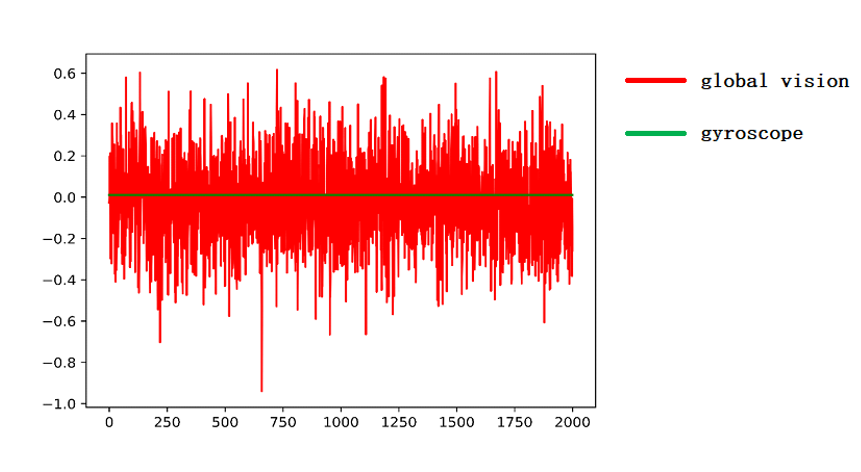
\includegraphics[width=0.8\textwidth]{Comparacao_cameras_giroscopio.png}
					\label{fig:comparison_cameras_gyroscope}
					\smallcaption{Fonte: Retirado de \textcite{tdpZJUNlict2020}}
				\end{figure}
		
			A equipe RoboTeam Twente em seu \textit{Team Description Paper} (\glsxtrshort{tdp}) de 2018 estima que o delay entre enviar um comando para o robô e notar uma resposta nas medições pode levar entre 80 e 150ms, dependendo da câmera utilizada \cite{tdptwente2018}. Por conta disso, faz-se necessário um sistema de localização que possua um delay relativamente menor para que o controle de posição dos robôs seja feito adequadamente.
			
			É notável que o sistema de câmeras da categoria \glsxtrshort{ssl} facilita a aquisição dos dados de posição, visto que ele já entrega para os times o posicionamento de todos os robôs e da bolinha. Apesar disso, para realizar o controle dos robôs de maneira robusta e qualificada é necessária a utilização de um sistema de localização embarcado que realize estimativas de posicionamento por conta do tempo de atualização dos dados das câmeras ser relativamente alto para a dinamicidade da partida.
			
			\subsection{Fusão de sensores na \glsxtrlong{ssl}} \label{sec:fusao_sensores_ssl}
			
				A fusão de sensores aplicada na categoria \glsxtrshort{ssl}, principalmente para localização dos robôs em campo numa partida, é justificada pela dinamicidade em que as jogadas acontecem por conta da velocidade máxima imposta na bola de jogo para realização de passes e chutes \cite{rules}, além do problema já abordado da taxa de atualização das posições capturadas pelo sistema global de câmeras.
				
				Por conta da complexidade de trabalhar com diversas habilidades, como localização, navegação e controle, de forma embarcada, grande parte das equipes prefere executar o controle de posicionamento no computador central de estratégia, utilizando somente os dados adquiridos do sistema global de visão, e enviando para os robôs, via rádio, a velocidade local que cada um deles deve impor \cite{ubc_thunderbots_2015, immortals_2023}. Assim, de forma embarcada os robôs precisam somente de um feedback das rodas por meio de encoders, por exemplo, para manter um controle de velocidade delas.
				
				Apesar de ser um sistema mais simples de implementar, o controle de posição dos robôs no computador central acaba levando a uma menor performance comparado com a utilização do controle embarcado \cite{ubc_thunderbots_2015}, muito por conta do delay inerente para atualização das imagens do sistema global de câmeras da liga. Entre um frame e outro, por conta da alta velocidade da bola em jogo, somado com o delay de envio e recebimento dos dados via rádio-frequência, há um aumento de dificuldade para realização de certas jogadas e habilidades \cite{immortals_2023}.
				
				Para solucionar o problema do delay entre pacotes do sistema de visão global da liga, a fusão de sensores passou a ser utilizada por equipes que, nos anos seguintes, demonstraram uma qualidade de jogo superior \cite{zjunlict_2018, tigers_2013, ubc_thunderbots_2015, ubc_thunderbots_2017, immortals_2023, parsian_2015}, a fim de aumentar a realização de habilidades de forma embarcada no robô. Portanto, um sistema de localização preciso e com baixa taxa de atualização é necessário, utilizando dados mais confiáveis na malha de controle.
				
				Em \textcite{immortals_2023} é feita uma fusão de sensores para orientação entre os dados do sistema de visão e os dados da \glsxtrshort{imu}, melhorando a qualidade da orientação predita. Em \textcite{parsian_2019} a fusão de sensores também é feita especialmente para a orientação, sendo que a equipe coloca que, comparado com o SSL-Vision, a fusão de sensores é mais acurada.
				
				A partir disso, é notória a melhoria de performance levando as habilidades do robô, como localização e navegação, para o microcontrolador do robô. A informação dos sensores presentes nos robôs e alta taxa de processamento permitem que o robô tenha melhores estimativas de localização em campo entre um frame e outro do sistema global de câmeras, aumentando a performance dos robôs.
		
	\section{SENSORES} \label{sec:sensores}
	
		A utilização de sensores é parte essencial para o funcionamento correto de um robô. Segundo \textcite{de2017tipos}, o mais predominante em robôs industriais são robôs projetados para realizarem operações pré-programadas, que acabam não usufruindo de sensores para atingirem seu objetivo. Entretanto, para robôs mais complexos, os sensores acabam introduzindo um maior nível de inteligência para poder interagir com o meio que está inserido por meio de atuadores.
		
		Também de acordo com \textcite{de2017tipos}, a utilização de sistemas sensoriais faz com que robôs sejam mais facilmente adaptáveis a uma maior gama de tarefas, atingindo um maior grau de universalidade, diferente dos robôs pré-programados, que acabam realizando apenas uma única função. Um robô que, a partir da leitura dos sensores, possui sensações tal como um humano, é mais facilmente treinado para realização de tarefas complexas.
		
		Portanto, essa seção visa apresentar as diferentes categorias de sensores, tal como explicar o funcionamento geral dos sensores a serem utilizados neste trabalho e como eles devem ser calibrados para conseguir aproveitar o melhor dos dados apresentados por eles. Os sensores descritos nessa seção são os usualmente utilizados pelos robôs da \glsxtrshort{ssl}, por conta da configuração do sistema global de visão e do limite de tamanho descrito em regra.
		
		\subsection{Tipos de sensores}		
		
			De acordo com \textcite{sensorFusionKalmanFilter}, o sensores podem ser divididos em duas categorias principais: internos e externos. Essa diferenciação diz respeito a partir de onde vem a informação lida pelo sensor, ou seja, se é do mundo externo ou se é internamente do próprio robô.
			
			Sensores internos fornecem informações sobre parâmetros internos do robô, ou seja, medem variáveis físicas dele, como a velocidade e o sentido de rotação de um motor, ou o ângulo de uma junta, como exemplos. Alguns possíveis sensores que fazem parte desse tipo são: encoder, giroscópio, acelerômetro, bússolas.
			
			Já os sensores externos medem a relação entre o robô e o ambiente em que ele está inserido, que podem ser objetos naturais ou artificiais, como por exemplo a distância do robô até um objeto ou medidas químicas do ambiente. Alguns possíveis sensores que fazem parte desse tipo são: sensores de contato (bumpers), sensores de distância como laser, sonar e radar, entre outros.
			
			Ambos sensores possuem vantagens e desvantagens. Para períodos curtos de tempo, as medições de sensores internos são bem acuradas, embora a longo prazo as medidas normalmente passam a ter desvios e erros. Ao contrário disso, os sensores externos não tem problemas de desvio do sinal ao passar do tempo, mas as medidas deles normalmente não estão sempre disponíveis, ou seja, possuem um período grande para atualizarem suas medidas.
			
			Portanto, para obter resultados ótimos, ambos sensores são normalmente combinados, juntando as qualidades de ambos e fazendo com que as desvantagens deles sejam superadas. Por conta do erro de ambos os sensores, é realizada uma fusão das medidas dos dois tipos de sensores, o que irá produzir uma estimativa desejada da posição do robô.
			
			No caso deste projeto, os seguintes sensores foram utilizados e explicados de maneira mais aprofundada: câmera, encoder, giroscópio e acelerômetro.
			
			\subsection{Sistema de câmeras} \label{sec:sensores_cameras}
			
				A câmera é um instrumento cujo uso em aplicações na área da robótica tem crescido bastante. Mapeamento, localização, navegação, desvio de obstáculos, reconhecimento de objetos e inspeção de qualidade são só alguns exemplos de possíveis utilizações de câmeras para realização de tarefas por parte de robôs. No centro dessa ascensão das câmeras está a evolução tanto dos processadores quanto dos algoritmos de visão computacional avançados.
				
				Segundo \textcite{cameras_technexion}, câmeras são cruciais no campo da robótica guiada por visão por aperfeiçoar as habilidades de percepção. Um robô pode aprender muito sobre seu arredor a partir dos dados visuais que câmeras coletam. Robôs podem obter informações valiosas desses dados utilizando diferentes métodos de processamento, permitindo que o robô enxergue, compreenda e interaja com o ambiente de uma maneira mais profunda.
				
				No caso deste projeto, a utilização de câmeras se dá externamente aos robôs dentro da categoria SSL da RoboCup, já que o sistema de visão não é embarcado nos robôs, embora haja estudos para alocar uma câmera dentro dos robôs da categoria de pequeno porte, como trazido por \textcite{melo2022embedded}.
				
				Detalhando um pouco mais o sistema de visão por câmeras da categoria SSL da RoboCup, atualmente utiliza-se uma ou duas câmeras, dependendo se o campo é da divisão A ou da divisão B. Independente do caso, a câmera fica posicionada acima do campo a 6 metros de altura e fica conectada a um computador central. Nele, a imagem é recebida, tratada e processada, identificando a posição da bola e dos robôs a partir do padrão de cor posicionado na parte de cima dos robôs, como é possível observar na Figura \ref{fig:color_patterns} as 16 diferentes combinações possíveis \cite{10.1007/978-3-642-11876-0_37}.
				
				\begin{figure}[!htb]
					\centering
					\caption{Padrões de cores para identificação dos robôs.} 
					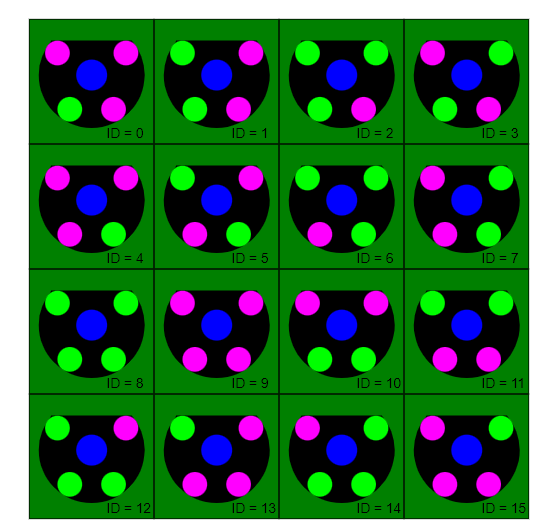
\includegraphics[width=0.5\textwidth]{Padrao_de_cores.eps}
					\label{fig:color_patterns}
					\smallcaption{Fonte: \textcite{rules}}
				\end{figure}
			
				Tanto o computador onde as imagens são processadas quanto o computador de cada uma das equipes estão conectados numa mesma rede. Assim, após o processamento das imagens, as posições dos robôs e da bola são passadas para as equipes pela rede, por isso o sistema de visão é dito compartilhado, pois ambas as equipes recebem as mesmas informações.
			
			\subsection{Encoder}\label{sec:sensores_encoders}
				
				Encoders são dispositivos utilizados a fim de medir o estado interno e a dinâmica de um robô móvel. Eles possuem uma vasta gama de aplicações fora da robótica e, por conta disso, robôs se aproveitaram dos benefícios da alta qualidade e baixo custo de sensores que oferecem uma excelente resolução de leitura. No mercado existem alguns diferentes tipos de encoders, como os ópticos e magnéticos. 
				
				No caso deste projeto, é utilizado um encoder do tipo óptico. Segundo \textcite{siegwart2011introduction}, este tipo de encoder se tornou o dispositivo mais popular para medição de velocidade e posição angulares de um motor, do eixo de uma roda ou mecanismo de direção.
				
				Um encoder óptico é basicamente um picador de luz mecânico que produz uma certa quantidade de pulsos na forma de um seno ou quadrado para cada revolução. No caso, o sensor consiste de uma fonte de iluminação, uma "grade" fixa que mascara a luz, um disco rotor com uma grade óptica fina que gira com o eixo e um detector óptico fixo. Ao passo que o rotor se movimenta, a quantidade de luz atingindo o detector óptico varia baseado no alinhamento das grades fixas e móveis. É possível observar a montagem e ter uma melhor ideia do funcionamento de um encoder óptico com a Figura \ref{fig:optical_encoder}.
				
				\begin{figure}[!htb]
					\centering
					\caption{Ilustração da montagem e funcionamento de um encoder óptico.} 
					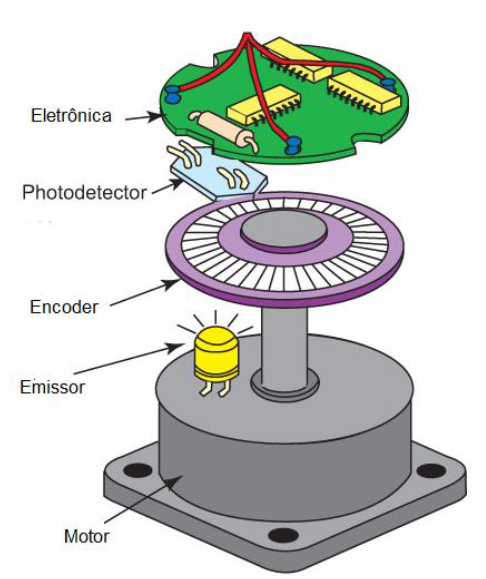
\includegraphics[width=0.5\textwidth]{encoder_optico.png}
					\label{fig:optical_encoder}
					\smallcaption{Fonte: Adaptado de \textcite{opticalencoder}}
				\end{figure}
				
				O projeto RoboFEI utiliza motores brushless da empresa Maxon\textregistered, no caso um motor brushless EC 45 com $50W$ acoplado em cada uma das rodas \cite{ec45_maxon}. Já o encoder utilizado é da empresa US Digital\textregistered \cite{e4t_encoder}, no caso é utilizado um encoder do modelo E4T por roda também, sendo que eles ficam acoplados diretamente ao eixo do motor.
				
				Cada encoder está ligado a um timer do microcontrolador utilizado em cada robô para realizar a contagem de pulsos do sensor. Seguindo a Equação \eqref{eq:velocidade_roda_encoder}, pode-se determinar a velocidade de rotação de cada roda em rpm, conhecendo a contagem de pulsos realizada, o intervalo de tempo (em segundos), a transmissão envolvida no conjunto roda-motor e a resolução de leitura do encoder (quantidade de pulsos por volta).
				
				\begin{equation}\label{eq:velocidade_roda_encoder}
					\begin{split}
						&\text{Rotação} = \frac{\text{Pulsos}}{\text{Transmissão} \times \text{Pulsos por volta}} \\
						&\text{Velocidade} = \frac{\text{Rotação} \times 60}{\Delta t}
					\end{split}
				\end{equation}
			
			\subsection{Giroscópio} \label{sec:sensores_giroscopio}
			
				Giroscópios também são um dos principais sensores utilizados em robôs para realização de tarefas básicas como navegação. De acordo com \textcite{jeremydingman2020}, eles são componentes essenciais de sistemas complexos utilizados em todas aplicações aeroespaciais, industriais e na área da robótica. Giroscópios auxiliam desde aviões e barcos até drones e carros autônomos a navegarem.
				
				Segundo \textcite{s17102284}, giroscópios são dispositivos montados em uma estrutura e capazes de detectar uma velocidade angular se a estrutura estiver girando. Esse sensor pode ser utilizado de forma sozinha ou pode estar incluso em um sistema mais complexo, como uma bússola giroscópica, uma \acrshort{imu} (\textit{Inertial Measurement System}, do inglês) ou um INS (\textit{Inertial Navigation System}, do inglês), por exemplo.
				
				No livro '\textit{Introduction to Autonomous Mobile Robot}', os autores trazem que giroscópios são sensores de direção que preservam sua orientação em relação a um \textit{frame} de referência fixo \cite{siegwart2011introduction}. Por isso, eles fornecem uma medida absoluta de orientação de um sistema móvel. 
				
				Também de acordo com \textcite{siegwart2011introduction}, os giroscópios são divididos em duas categorias: mecânicos e ópticos. Os primeiros dependem das propriedades de um rotor de rotação rápida, propriedade chamada de precessão giroscópica. Já os segundos são sensores de velocidade angular que utilizam dois feixes de luz monocromáticos, ou lasers, emitidos de uma mesma fonte
				
				No caso desse projeto, o giroscópio utilizado é o I3G4250D, que é um sensor de velocidade angular de baixo consumo de energia capaz de realizar medidas nos 3 eixos \cite{datasheet_gyro}. Esse componente inclui o sensor e uma interface capaz de fornecer a medida de velocidade angular ao mundo externo por meio de uma interface digital \glsxtrshort{i2c} (do inglês, \glsxtrlong{i2c}) ou \glsxtrshort{spi} (do inglês, \glsxtrlong{spi}).
			
			\subsection{Acelerômetro} \label{sec:sensores_acelerometro}
			
				O acelerômetro é mais um dos sensores que é utilizado para que o robô possua a habilidade de entender sua localização no espaço, o que é criticamente importante para alcançar com êxito o objetivo determinado para o robô desenvolvido.
			
				Segundo \textcite{NISTLER2011413}, grande parte dos sistemas de odometria para aplicações em robótica possuem acelerômetros. Estes continuamente medem a aceleração do robô, que é integrada para determinada a velocidade dele, e é integrado novamente para ter a medida da posição relativa ao ponto inicial.
				
				Entretanto, por conta da influência da gravidade, da força inercial de Coriolis \cite{persson1998we} e componentes rotacionais de aceleração, sistemas de odometria baseados em acelerômetros estão sujeitos a diversos erros dependendo do processamento das medidas do sensor. Também segundo \textcite{NISTLER2011413}, quando o robô se move numa superfície horizontal, a velocidade computada irá refletir a velocidade real do robô, mas em superfícies inclinadas, a velocidade medida irá incluir esses erros listados, que não fazem parte da velocidade real.
			
				De acordo com \textcite{dadafshar2014accelerometer}, a operação básica de um acelerômetro recai na Segunda Lei de Newton, a qual diz que a aceleração de um corpo é diretamente proporcional, e na mesma direção, a força resultante atuante no corpo, e inversamente proporcional à massa do corpo, descrito na Equação \eqref{eq:newton_second_law}.
				
				\begin{equation}\label{eq:newton_second_law}
					\overrightarrow{a}(m/s^2) = \frac{\overrightarrow{F}(N)}{m(kg)}
				\end{equation}
			
				Nota-se que a aceleração gera uma força que é capturada pelo mecanismo de detecção de força do acelerômetro. Portanto, o acelerômetro na verdade realiza medidas de força, e não aceleração, mas ele acaba medindo a aceleração indiretamente por meio da força aplicada em um de seus eixos.
				
				De acordo com \textcite{siegwart2011introduction}, os acelerômetros são separados dependendo do princípio físico utilizado para realizar a medição da deflexão da massa interna do sensor. Um mecanismo comum de detecção utilizado é a detecção por capacitância, que mede a deflexão ao medir a capacitância entre uma estrutura física e a massa interna. Outra alternativa de medição é a piezoelétrica, que é baseada na propriedade de certos cristais em gerarem tensão quando um estresse mecânico é aplicado neles, no caso a massa interna é posicionada no cristal e, quando uma força externa é aplicada, a massa induz uma tensão que pode ser medida.
				
				No caso desse projeto, o acelerômetro utilizado é o LSM303AGR, que é um sensor digital de aceleração linear capaz de realizar medidas nos 3 eixos, e é um sensor digital magnético nos 3 eixos também \cite{datasheet_accel}. O componente inclui uma interface serial \glsxtrshort{i2c}, que suporta os modos padrão e rápido com 100kHz e 400kHz, ou uma interface serial padrão \glsxtrshort{spi}.
				
			\subsection{\textit{Inertial Measurement Unit} (\glsxtrshort{imu})}
			
				A \acrshort{imu}, é um dispositivo que utiliza giroscópios e acelerômetros para estimar a posição, velocidade e aceleração relativos do veículo em movimento. Este componente se tornou comum em aviões e barcos, por exemplo, por estimar a posição do veículo em seis graus de liberdade, no caso: posição(x, y, z) e orientação (\textit{roll}, \textit{pitch}, \textit{yaw}) \cite{siegwart2011introduction}.
				
				Além disso, as \acrshort{imu}s comercializadas também estimam velocidade e aceleração. Considerando que a \acrshort{imu} possua 3 acelerômetros ortogonais e 3 giroscópios ortogonais, os dados do segundo são integrados para estimar a orientação do veículo enquanto os dados do primeiro são utilizados para estimar a aceleração instantânea do veículo.
				
				A aceleração é transformada para o frame da navegação local por meio da estimativa atual da orientação do veículo relativo à gravidade. Portanto, o vetor gravidade pode ser subtraído das medidas, resultando numa aceleração que é integrada para obter a velocidade e integrada novamente para obtenção da posição. Para sobrepor o problema da necessidade de conhecer a velocidade inicial, a integração é tipicamente iniciada no repouco, ou seja, velocidade igual a zero.
				
				\acrshort{imu}s são extremamente sensíveis na questão de erros de medidas tanto em relação ao giroscópio quanto ao acelerômetro. Por exemplo, o desvio no giroscópio inevitavelmente prejudica a estimativa da orientação do veículo relativa à gravidade, o que resulta numa cancelamento incorreta do vetor da gravidade. Além disso, por exemplo, os dados do acelerômetro são integrados duplamente para obter a posição, logo qualquer resíduo do vetor gravidade gera um erro que é duplamente integrado na posição. Por conta desse problema de desvio, é necessário alguma referência de fonte externa de medida, como um GPS (do inglês, \glsxtrlong{gps}), câmera ou \acrshort{lidar} (do inglês, \glsxtrlong{lidar}).
		
		\subsection{Calibração dos sensores}\label{sec:calibracao_sensores}
		
		O mercado mundial de sensores vem expandindo numa alta taxa ao longo dos últimos anos empurrado pelo desenvolvimento de outras tecnologias que fazem uso desses componentes, como robôs, carros autônomos, tecnologias de energia verde e internet das coisas (\textit{Internet of Things}, do inglês), por exemplo. De acordo com \textcite{sensor_market}, o mercado global de sensores estima o crescimento de \$179.7 bilhões em 2023 para \$300.5 bilhões até 2029.
		
		Entretanto, apesar do forte avanço do mercado de sensores mundial, de acordo com \textcite{calibration_av}, a calibração de sensores é um dos tópicos menos discutidos no desenvolvimento de sistemas autônomos, apesar de ser o bloco de fundação do sistema e de seus sensores, e é uma etapa de processamento necessária antes da implementação de técnicas de fusão sensorial.
		
		De acordo com \textcite{lv2020targetless}, a calibração dos sensores é uma parte fundamental para o desenvolvimento de um projeto de fusão multi-sensorial. Isso se dá pelo fato do aumento da qualidade dos dados lidos pelos sensores e, assim, uma consequente melhoria na confiabilidade do sistema como um todo. Em sistemas como robôs e carros autônomos, isso pode determinar diretamente a segurança e viabilidade deles.
		
		No caso desse projeto, a calibração foi realizada para os sensores giroscópio e acelerômetro, que são chamados de sensores inerciais microeletromecânicos (\glsxtrshort{mems}, do inglês), cujo desenvolvimento foi o protagonista para o crescimento de sistemas de navegação inerciais (\glsxtrshort{ins}, do inglês) e superar os pontos negativos de outros sensores, como o GPS, que são consideravelmente lentos para atualizar a informação.
		
		Segundo \textcite{9181212}, sensores inerciais \glsxtrshort{mems} são utilizados preferencialmente por conta tanto do seu baixo custo quanto do seu reduzido tamanho. Entretanto, uma grande desvantagem deles é a sua característica de grande erro. Por conta disso, a calibração desses sensores é necessária para garantir seu bom funcionamento num \glsxtrshort{ins}, compensando a parte determinística de seu erro.
		
			\subsubsection{Calibração do acelerômetro} \label{sec:calibracao_acelerometro}
			
			A calibração do componente acelerômetro pode ser dividida em duas partes diferentes: compensação do \textit{bias} da leitura de cada um dos eixos e a calibração da inclinação da IMU em relação ao frame do robô, este que acontece por conta da solda do componente ou de algum fator mecânico, o que faz com que os eixos do robô e do componente provavelmente não sejam compatíveis.
			
			A calibração é realizada pelo método proposto por \textcite{menezes2020triaxial}, que é baseado numa estimativa pelo método dos mínimos quadrados. No caso, o método é uma adaptação de uma técnica utilizada para calibração de magnetômetros (dispositivos que medem a força do campo magnético), alterando que ao invés de medir o campo magnético da Terra é medida a aceleração local da gravidade. Além disso, o método para acelerômetros deve ser realizado enquanto o componente esteja estacionário ou submetido a rotações que não produzam forças centrípetas detectáveis.
			
			De acordo com \textcite{menezes2020triaxial}, há 4 componentes que compõe o erro de um acelerômetro, que são:
			
			\begin{itemize}
				\item \textbf{Desvio:} Chamado de \textit{bias} em inglês, o desvio é o componente mais comum na calibração de acelerômetro. Esse tipo de erro adiciona um deslocamento nas leituras do sensor.
				
				\item \textbf{Fatores de escala:} Esse componente corrompe as medições ao escalar incorretamente elas.
				
				\item \textbf{Desalinhamentos:} Também conhecido como não-ortogonalidades ou erros de acoplamento cruzado, esse componente diz respeito à disposição angular entre os eixos do corpo e os eixos reais de sensibilidade. O efeito prático desses desalinhamentos é que um sensor acaba sentindo (leia-se, medindo) a aceleração dos outros eixos, portanto a leitura não é completamente relacionada ao seu respectivo eixo.
				
				\item \textbf{Ruídos aleatórios:} Este componente é assumido como ruído branco e com média zero seguindo uma distribuição Gaussiana. Os autores colocam que como a aceleração é realizada no domínio dela própria nenhuma integração numérica é realizada, logo esses processos aleatórios podem ser desconsiderados.
			\end{itemize}
			
			De acordo com \textcite{hassan2020field}, apenas os três primeiros itens são considerados durante a modelagem de erros sistemáticos. Assim, a leitura de um acelerômetro pode ser descrita conforme a Equação \eqref{eq:equacao_geral_accel}, em que $a$ é o vetor que representa as acelerações calibradas nos 3 eixos, $S$ é a matriz que representa os erros de fator de escala e desalinhamento (no caso, na diagonal principal estão os dados do erro de fator de escala, enquanto o restante dos valores são os erros de desalinhamento), o vetor $B$ representa os desvios do sensor em cada eixo, indicados como $b$, enquanto $\tilde{a}$ representa os dados crus do sensor nos 3 eixos. Os índices $x$, $y$ e $z$ representam os eixos em questão e, quando eles estão conjugados (como $xy$, por exemplo) representam influência mútua.
			
			\begin{equation}\label{eq:equacao_geral_accel}
				\begin{split}
					&\quad \quad a = S(\tilde{a} - B) \\
					\begin{bmatrix}
						a_x \\ a_y \\ a_z
					\end{bmatrix} = 
					&\begin{bmatrix}
						S_x & S_{xy} & S_{xz} \\ S_{xy} & S_y & S_{yz} \\ S_{xz} & S_{yz} & S_z
					\end{bmatrix} \left(
					\begin{bmatrix}
						\tilde{a}_x \\ \tilde{a}_y \\ \tilde{a}_z
					\end{bmatrix} + 
					\begin{bmatrix}
						b_x \\ b_y \\ b_z
					\end{bmatrix}\right)
				\end{split}
			\end{equation}
			
			Como dito anteriormente, o método se baseia que durante o repouso do sensor, o módulo da aceleração nos três eixos deve ser igual à aceleração da gravidade, como descrito na Equação \eqref{eq:calibracao_gravidade}.
			
			\begin{equation} \label{eq:calibracao_gravidade}
				a_{x}^{2} + a_{y}^{2} + a_{z}^{2} = g^{2}
			\end{equation}
			
			A partir disso, devem ser recolhidas amostras do sensor em diferentes posições para que a calibração tenha uma maior eficiência, já que em \textcite{menezes2020triaxial} é mostrado que o método consegue melhores resultados ao aumentar a quantidade de amostras, sendo que os autores colocam que 9 é a quantidade mínima nesse caso.
			
%			\begin{equation} \label{eq:calibracao_bias_gravidade}
%				(a_x + b_x)^{2} + (a_y + b_y)^{2} + (a_z + b_z)^{2} = g^{2}
%			\end{equation}
%			
%			\begin{equation} \label{eq:desenvolvimento_calibracao_grav}
%				\begin{split}
%					&b_x^{2} + b_y^{2} + b_z^{2} - g^{2} - 2a_xb_x - 2a_yb_y - 2a_zb_z = - (a_x^{2} + a_y^{2} + a_z^{2}) \\
%					&P = b_x^{2} + b_y^{2} + b_z^{2} - g^{2} \\
%					&Q = -2b_x \\
%					&R = -2b_y \\
%					&S = -2b_z \\
%					&P + Qa_x + Ra_y + Sa_z = - (a_x^{2} + a_y^{2} + a_z^{2})
%				\end{split}
%			\end{equation}
%			
%			Assim, pode-se escrever a Equação \eqref{eq:desenvolvimento_calibracao_grav} conforme a Equação \eqref{eq:calibracao_geral_grav} na forma de matrizes e vetores, em que as matrizes A e B dependem da quantidade de amostras utilizadas para realizar a calibração.
%			
%			\begin{equation}\label{eq:calibracao_geral_grav}
%				\begin{split}
%					&B = A'\overrightarrow{x} \\
%					&\overrightarrow{x} = \begin{bmatrix}
%						P & Q & R & S
%					\end{bmatrix}^T \\
%					&A = \begin{bmatrix}
%						1 & a_{x1} & a_{y1} & a_{z1} \\
%						1 & a_{x2} & a_{y2} & a_{z2} \\
%						\vdots & \vdots & \vdots & \vdots & \\
%						1 & a_{xn} & a_{yn} & a_{zn} \\
%					\end{bmatrix} \\
%					&B = \begin{bmatrix}
%						- (a_{x1}^{2} + a_{y1}^{2} + a_{z1}^{2}) \\
%						- (a_{x2}^{2} + a_{y2}^{2} + a_{z2}^{2}) \\
%						\vdots \\
%						- (a_{xn}^{2} + a_{yn}^{2} + a_{zn}^{2}) \\
%					\end{bmatrix}
%				\end{split}
%			\end{equation}
			
		\subsubsection{Calibração do giroscópio}\label{sec:calibracao_giroscopio}
		
		A calibração do giroscópio segue as mesmas ideias da calibração do acelerômetro. Entretanto, em \textcite{hassan2020field} somente o fator de escala e os desvios são considerados no estudo como fontes de erro.
		
		Assim, a relação entre a velocidade angular real e a velocidade angular medida pode ser observada com a Equação \eqref{eq:equacao_geral_gyro}, em que $\omega$ é o vetor que representa as velocidades angulares calibradas nos 3 eixos, enquanto $\tilde{\omega}$ representa o vetor com os dados crus do sensor nos 3 eixos.
		
		\begin{equation}\label{eq:equacao_geral_gyro}
			\begin{split}
				&\quad \quad \omega = S(\tilde{\omega} - B) \\
				\begin{bmatrix}
					\omega_x \\ \omega_y \\ \omega_z
				\end{bmatrix} = 
				&\begin{bmatrix}
					S_x & S_{xy} & S_{xz} \\ S_{xy} & S_y & S_{yz} \\ S_{xz} & S_{yz} & S_z
				\end{bmatrix} \left(
				\begin{bmatrix}
					\tilde{\omega}_x \\ \tilde{\omega}_y \\ \tilde{\omega}_z
				\end{bmatrix} + 
				\begin{bmatrix}
					b_x \\ b_y \\ b_z
				\end{bmatrix}\right)
			\end{split}
		\end{equation}
		
		Entretanto, como nesse caso as amostras também devem ser tomadas em repouso, a aceleração real deve ser considerada nula. Portanto, os erros de fator de escala podem ser desconsiderados no caso desse projeto, sendo necessário apenas descobrir os desvios do sensor.
				
	\chapter{LOCALIZAÇÃO DE ROBÔS MÓVEIS}\label{sec:chapter_localizacao_robos_moveis}
	
		Nessa seção serão comentadas as questões que envolvem como um todo a localização de robôs móveis. No caso, serão discutidos a questão geral da localização de robôs e seus principais problemas, suas diferentes instâncias e a questão da informação disponível para localização de robôs.
		
		\section{O problema da localização}
		
			A navegação é uma das competências mais desafiadoras necessárias em um projeto de robô móvel. De acordo com \textcite{siegwart2011introduction}, o sucesso da navegação depende do sucesso de 4 pilares principais: percepção, localização, cognição e controle de movimento. O primeiro é como o robô interpreta os dados dos sensores para extrair dados significativos para seus objetivos. O segundo é a determinação da posição do robô no ambiente. O terceiro é sobre como o robô deve decidir suas ações para atingir seus objetivos. O quarto define como o robô deve modelar as saídas dos seus motores para atingir a trajetória desejada.
			
			Este trabalho se debruça no pilar da localização basicamente. O problema da localização consiste em responder a pergunta "Onde estou?" do ponto de vista do robô, o que quer dizer que o robô precisa descobrir sua localização relativa ao ambiente em que ele se encontra. Quando fala-se sobre posição, quer dizer sobre as coordenadas $x$ e $y$ do robô, tal como sua orientação no sistema de coordenadas global.
			
			Como dito em \textcite{thrun2001robust}, o problema de localização de um robô é algo muito importante, sendo um componente chave em diversos sistemas robóticos autônomos de sucesso. Se um robô não sabe onde está relativamente ao ambiente, a tomada de decisão do que fazer é praticamente impossível, o robô precisa ter pelo menos uma certa noção de onde ele está para poder operar e agir de maneira certa. Segundo \textcite{borenstein1997mobile}, saber exatamente a posição de um robô é um problema fundamental em aplicações de robôs móveis para prover realmente capacidades autônomas.
			
			Problemas de localização são caracterizados pelo tipo de conhecimento que está disponível inicialmente e durante a execução. Basicamente, há três tipos de problemas de localização com diferentes graus de dificuldade, que são:
			
			\begin{itemize}
				\item \textbf{Rastreio de posição:} Assume que a posição inicial do robô é conhecida, logo a localização do robô pode ser conseguida ao acomodar o ruído na movimentação do robô, geralmente o efeito desse ruído sendo pequeno. Esse problema é dito como local, já que a incerteza é local e restrita a uma região perto da posição verdadeira do robô, além de que a incerteza é geralmente aproximada por uma distribuição unimodal, como uma gaussiana.
				
				\item \textbf{Localização Global:} Aqui a posição inicial do robô é desconhecida, já que o robô é inicialmente colocado em algum local do ambiente, mas há a falta do conhecimento de onde é o local, ou seja, ele precisa se localizar do zero. As abordagens para localização global não podem assumir limite no erro da posição, assim como assumir distribuição probabilística unimodal é geralmente inapropriado.
				
				\item \textbf{Problema do sequestro de robô:} É uma variante do problema de localização global, mas nesse caso o robô sabe onde está localizado e de repente é "sequestrado" para outra localização sem que o robô esteja ciente disso. O problema é o robô detectar que foi sequestrado e, em seguida, descobrir sua nova localização. A importância prática disso, apesar de ser algo que não aconteça frequentemente, decorre que grande parte dos algoritmos de localização não garantem que nunca falharão.
			\end{itemize}
			
		\section{Os desafios da localização}
		
			Ao falar dos desafio da localização, \textcite{siegwart2011introduction} falam sobre a situação hipotética de utilizar um GPS (do inglês, \textit{Global Positioning System}) em um robô móvel e como o problema de localização estaria evitado, já que o sensor informaria a posição exata interna e externamente e a questão "Onde estou?" sempre estaria respondida. Porém, infelizmente, esse sensor não é prático, já que o GPS atual tem uma acurácia de alguns metros na época de publicação do livro, o que é inaceitável para localizar robôs móveis, além de não funcionar em ambientes internos. Atualmente, a acurácia já está em centímetros para aplicações externas, por exemplo. 
			
			Indo mais a fundo nas limitações do GPS, a localização é mais do que saber a posição absoluta do robô em relação à Terra, é também saber a sua localização relativa em respeito a, por exemplo, humanos, considerando a situação de um robô que tem que interagir com pessoas. Além do mais, se o robô planeja atingir uma localização específica, talvez seja necessário adquirir um modelo do ambiente (um mapa) e identificar a posição relativa do robô nele. 
			
			Por conta da falta de acurácia e imperfeição de sensores e atuadores que a localização enfrenta desafios difíceis. Os principais aspectos que tornam o funcionamento de sensores e atuadores sub-ótimos são: ruído e \textit{aliasing} em sensores e ruído em atuadores.
			
			Sensores são a entrada fundamental do robô para o processo de percepção	e, portanto, o grau em que sensores podem discriminar o estado em relação ao mundo que o robô se encontra é crítico. O ruído induz uma limitação na consistência das leituras de um sensor em um mesmo estado do ambiente. Geralmente, a fonte de problemas com ruídos em sensores é que algumas características não são capturadas pelo robô e, portanto, ignoradas. Resumindo, o ruído em sensores reduzem a informação útil de suas leituras. Uma saída para isso é considerar várias leituras, aplicando fusão temporal ou fusão de diversos sensores para aumentar a qualidade geral da informação de entrada de robôs.
			
			Outra deficiência em relação aos sensores é a questão do \textit{aliasing}, que os leva a colherem pouco conteúdo informativo, o que acaba agravando o problema da percepção e, assim, dificultando a localização de robôs móveis. Um exemplo que mostra bem a questão do \textit{aliasing}, trazido em \textcite{siegwart2011introduction}, é que a utilização de um sonar em um robô móvel não traz a informação se algo que foi detectado é um humano que o robô deveria dizer "com licença" ou um objeto inanimado que o computador deveria recalcular o trajeto para ultrapassar. Ou seja, a quantidade de informações é geralmente insuficiente para identificar a posição do robô a partir de uma leitura de percepção única.
			
			Já o ruído em atuadores cai na questão de que uma única ação tomada por um robô móvel pode ter diferentes resultados possíveis, mesmo que da perspectiva do robô o estado inicial antes da ação tomada é bem conhecido. Em resumo, atuadores em robôs móveis introduzem incerteza sobre o estado futuro, como por exemplo, o ato de andar tende a aumentar a incerteza de um robô. A maior fonte de erro geralmente reside em um modelo incompleto do ambiente, como por exemplo o fato de o modelo não levar em conta que as rodas de um robô podem escorregar ou que um humano pode empurrar o robô, ou seja, não leva em conta possíveis fontes de erros que não podem ser modeladas, resultando numa falta de acurácia entre o movimento físico do robô, a movimentação pretendida pelo robô e a estimativa de movimentação pelo sensor.
		
		\section{Informação disponível}
			
			Para determinar sua localização, um robô tem acesso a dois tipos de informação. Primeiro por meio de uma compreensão a priori obtida pelo próprio robô ou suprida por uma fonte externa numa fase chamada de inicialização. Segundo o robô obtém informação sobre o ambiente por meio de cada observação e ação realizadas durante a fase chamada navegação. 
			
			Em geral, a informação a priori fornecida ao robô descreve o ambiente pelo qual o robô está navegando, ou seja, especifica algumas características que são variantes no tempo e assim podem ser utilizadas para determinar a localização. Alguns exemplos desse tipo de informação podem ser mapas e relações causa-efeito.
			
			Robôs podem ter acesso a um mapa que descreve o ambiente em que está localizado. Os mapas podem ser topológicos ou geométricos \cite{mendes2017perceccao}, o primeiro tipo descreve o ambiente em termos métricos, como por exemplo mapas de rodovias, já o segundo tipo descreve o ambiente em termos de características específicas em localizações e maneiras de ir de um local para outro. O mapa pode ser aprendido pelo robô previamente, ou fornecido por uma fonte externa, ou aprendido enquanto navega pelo ambiente. Já as relações causa-efeito fornecem informações a priori ao robô por meio de uma dada entrada de observação, dizendo ao robô onde ele está a partir delas.
			
			Robôs também tem acesso à chamada informação de navegação, que é o tipo de informação que o robô reúne de diferentes sensores enquanto navega pelo ambiente. Um robô tipicamente performa dois tipos de ações ao navegar: ele anda ou age no ambiente por um lado, e sente o ambiente por outro lado.
			
			Um sistema de locomoção consiste de rodas, pernas ou trilhos, ou qualquer coisa que faça o veículo se movimentar pelo ambiente. A maneira na qual um sistema de deslocamento muda a localização contém informação valorosa para realizar a estimativa da própria localização, ou seja, saber os efeitos de ações executadas pelo sistema indica diretamente a localização do veículo depois da execução dessas ações.
			
			O robô sente o ambiente por meio de sensores, que indicam a informação de uma situação momentânea, chamada de observação ou medição, ou seja, essa informação descreve uma situação do ambiente do robô em um certo momento. Observações feitas do ambiente providenciam informação sobre a localização do robô que é independente de uma estimativa de localização anterior, dando ênfase que a informação dessas medições vem da observação do ambiente ao invés do próprio robô.
	
	\section{FUSÃO DE SENSORES}
	
		\textcite{alatise2020review} trazem que robôs móveis autônomos estão se tornando mais proeminentes nos últimos tempos por conta do aumento de sua relevância e aplicações em diversas áreas, como em empresas, indústrias, hospitais, setor agrícola, realizando funções como carregamento de objetos pesados, monitoramento e busca. Por conta disso, a fusão de sensores vem sendo utilizada para solução de problemas como localização, mapeamento e navegação.
		
		A fusão de sensores é um tema que envolve uma grande multidisciplinaridade de áreas. Por conta disso, existem diversas definições do que é fusão de sensores na literatura, como a definição de \textcite{castanedo2013review} e \textcite{nagla2014multisensor}, que definem como o uso cooperativo de informação providenciada por diversos sensores a fim de ajudar no desempenho de uma determinada função. Trazendo mais para o campo da robótica, \textcite{luo2011multisensor} trazem que a fusão de multi sensores é uma tecnologia que realiza a combinação sinérgica de dados sensoriais de múltiplos sensores a fim de atingir inferências que não são possíveis com os sensores operando separadamente.
		
		A ideia de unir sensores não é recente na história da humanidade, um exemplo muito bom para mostrar esse fato é que, de acordo com \textcite{hall1997introduction}, humanos e animais desenvolveram a capacidade de utilizar múltiplos sentidos para melhorar suas habilidades de sobrevivência, como no caso de um animal que não consegue ver ao redor de cantos ou por meio da vegetação, então o sentido de audição pode prover bons avisos de perigos. Assim, a fusão de sensores é naturalmente realizada por animais e humanos para uma melhor abordagem do ambiente ao redor e para identificação de ameaças.
		
		De acordo com \textcite{marton2013two}, a fusão de sensores é um método efetivo para solucionar o problema de localização precisa de robôs móveis. Nessa técnica, mais de um sensor é utilizado para obter a posição do robô e para uma combinação efetiva de diferentes medições a fim de gerar os estados estimados do sistema. Assim, a fusão de sensores permite a mitigação das limitações de diferentes sensores, obtendo uma posição mais precisa do robô.
		
		A seguir, nessa seção serão comentadas as vantagens e desvantagens de utilizar fusão de sensores em sistemas inteligentes, além de apresentar três tipos de classificação dos diferentes métodos e técnicas de fundir dados de múltiplos sensores em um sistema para melhor entendimento da técnica utilizada neste projeto.
		
		\subsection{Vantagens e Desvantagens}
		
			\textcite{fung2017sensor} trazem que a maioria dos sensores não geram diretamente um sinal de um fenômeno externo, mas sim através de diversas etapas de conversão. Por conta disso, o dado sensorial lido pelo usuário pode desviar da entrada real. O autor também coloca que existem algumas características de sensores que são inevitáveis, como velocidade e frequência de resposta, atraso e tempo de acomodação, e que acabam levando a diversas complicações, que são enfrentadas pela fusão de sensores. Além disso, existem outras características estáticas, como acurácia, precisão, resolução e sensibilidade, que podem ser facilmente geridas antes do processo de fusão.
			
			\textcite{fung2017sensor} trazem também que a maior parte dos sensores não são ideais e possuem desvios que podem vir junto da informação necessária, alguns deles podem ser considerados de uma fonte aleatória de ruído, que precisam de um processamento para redução, já outros são considerados sistemáticos correlacionados com o tempo, estes também podem ser melhorados se o erro é conhecido.
			
			Como comentado anteriormente, o principal propósito de sensores externos é prover ao sistema informação útil no que diz respeito a informações de interesse do ambiente. A fusão de dados de diferentes sensores traz diversas vantagens relacionadas a obtenção de informações mais precisas, que no caso são impossíveis de perceberem somente com os dados individuais. Segundo \textcite{alatise2020review}, os seguintes itens são as principais vantagens da fusão de dados de sensores.
			
			\begin{itemize}
				
				\item \textbf{Redução da incerteza:} os dados providenciados por sensores estão, por vezes, sujeitos a um nível de incerteza e discrepância. Assim, a fusão de dados de diferentes sensores reduz a incerteza ao combinar dados de inúmeras fontes. É, assim, imperativo compensar usando outros sensores ao fundir seus dados utilizando algoritmos de fusão.
				
				\item \textbf{Aumento na acurácia e confiabilidade:} integração de múltiplos sensores vai permitir que o sistema providencie informação inerente mesmo em caso de falha parcial em algum de seus módulos sensoriais.
				
				\item \textbf{Cobertura temporal e espacial estendida:} a área coberta por um sensor pode não ser coberta por outro sensor, portanto a medição de um é dependente do outro e ambos se complementam. Um exemplo em que ocorre isso é um sensor inercial, como acelerômetro e giroscópio, e visão, nesse caso a cobertura da câmera como sensor de visão não pode ser comparada com o uso do acelerômetro, que apenas pega medidas sobre a rota de navegação.
				
				\item \textbf{Resolução aprimorada:} o valor da resolução resultante de múltiplas medições independentes fundidas é melhor que a medição singular de um sensor.
				
				\item \textbf{Complexidade reduzida do sistema:} um sistema em que os dados do sensor são pré-processados por algoritmos de fusão, a entrada para a aplicação de controle pode ser padronizada de forma autônoma dos tipos de sensores empregados, assim simplificando a implementação e providenciando a opção de modificações no sistema de sensor relativo ao número e tipo dos sensores sem alterações do software aplicado.
				
			\end{itemize}
		
			Embora seja provado a qualidade da fusão de sensores, de acordo com \textcite{fung2017sensor}, existem alguns problemas associados com a criação de uma metodologia geral para fusão de diferentes sensores e eles se concentram em torno dos métodos utilizados para modelagem do erro ou incertezas no processo de integração dos dados, na informação sensorial e na operação do sistem em geral incluindo os sensores. Sendo assim, os seguintes itens são colocados pelo autor como potenciais problemas.
			
			\begin{itemize}
				\item \textbf{Registro dos dados:} sensores individuais possuem seus próprios frames de referência do qual os dados são calculados. Para que a fusão ocorra, os conjuntos de dados diferentes devem ser convertidos para um frame de referência comum, e assim alinhados juntos. Erro de calibração de sensores individuais deve ser abordado durante este estágio. Este problema acaba sendo crítico na determinação se a fusão funcionará ou não.
				
				\item \textbf{Incerteza nos dados sensoriais:} Diversos formatos de dados podem criar ruídos e ambiguidade no processo de fusão. Dados competitivos ou conflitivos podem ser resultados desses erros. A redundância dos dados de diversos sensores precisa estar engajada em reduzir a incerteza e aprender a rejeitar valores discrepantes se dados conflitivos são encontrados.
				
				\item \textbf{Dados incompletos, inconsistentes e falsos:} dados são considerados incompletos se os dados observados permanecem os mesmos independente do número de interpretações. Sensores inconsistentes são definidos como dois ou mais conjuntos de dados completos mas que possuem diferentes interpretações.
				
				\item \textbf{Associação de dados/Correspondência:} um aspecto da fusão de sensores é estabelecer se duas faixas de cada sensor representam o mesmo objeto, sendo isto necessário para saber como características de dados combinam de diferentes sensores, além de saber se podem ser discrepantes. 
				
				\item \textbf{Granularidade:} o nível de detalhes de diferentes sensores são dificilmente similares. Os dados podem ser esparsos ou densos, relativos a outros sensores. O nível dos dados pode ser diferente e isso deve ser abordado no processo de fusão.
				
				\item \textbf{Escalas de tempo:} sensores podem medir o mesmo ambiente em taxas diferentes. O tempo de chegada ao nó de fusão pode não coincidir por conta de atrasos de propagação no sistema. Em casos em que o algoritmo de fusão necessita do histórico dos dados, o quão rápido o sensor consegue prover o dado é diretamente relacionado à validade dos resultados.
			\end{itemize}
		
		\subsection{Classificação de técnicas}
			Após o entendimento do que é a fusão de sensores, como ela pode ajudar diferentes sistemas e alguns pontos dela que merecem certa atenção para evitar problemas, é necessário diferenciar as diversas técnicas que realizam essa função de unir dados de sensores. De acordo com \textcite{castanedo2013review}, esse tema é uma área multidisciplinar que envolve diferentes campos do conhecimento, portanto é difícil estabelecer uma classificação clara e estrita das diferentes técnicas. Por isso, foram escolhidas 3 maneiras para classificação dos diferentes métodos de fusão sensorial.
			
			\subsubsection{Classificação baseada na relação entre as fontes de dados}
				De acordo com \textcite{castanedo2013review}, a relação entre as fontes de dados é uma maneira de dividir as diferentes técnicas de fusão de sensores, separando nas seguintes três categorias.
				
				\begin{itemize}
					\item \textbf{Complementar:} é o caso de quando os sensores não dependem diretamente entre si, mas podem ser combinados de uma maneira que entreguem uma visão mais completa do fenômeno sendo observado. Ou seja, a informação providenciada pelas diferentes fontes representam diferentes partes do cenário. Um exemplo que pode ser colocado são câmeras em uma sala sendo que cada uma acaba observando partes disjuntas.
					
					\item \textbf{Competitiva:} também chamada de redundante, é o caso em que cada sensor entrega medidas independentes de uma mesma propriedade e, assim, as informações podem ser utilizadas a fim de obter uma informação global mais confiável. \textcite{visser1999organisation} ainda separam essa categoria em dois - a fusão de dados de diferentes sensores ou a fusão de medições de um mesmo sensor tomadas em diferentes instantes. Um exemplo é o caso de dados vindo de áreas sobrepostas em redes de sensores visuais.
					
					\item \textbf{Cooperativa:} é quando as informações fornecidas por dois sensores independentes são utilizadas para conseguir alguma informação que não estaria disponível com os sensores funcionando sozinhos. De acordo com \textcite{brooks1998multi}, é a fusão mais difícil de projetar, já que o dado resultante está suscetível a problemas de todos os sensores sendo fundidos, o que geralmente diminui a acurácia e confiabilidade em relação às outras categorias. Um exemplo é uma fusão de dados multi-modal entre áudio e vídeo para gerar uma informação mais complexa.
				\end{itemize}
				
				De acordo com essa classificação, esse projeto transitou entre os tipos complementar e competitiva, já que depende da combinação de sensores a ser empregada. Por exemplo, o encoder e o giroscópio podem prover observações sobre a velocidade angular, o que é uma fusão competitiva, mas há combinações que estão no caso de fusão complementar por apresentarem dados diferentes de uma mesma cena.
			
				A Figura \ref{fig:classificacao_fusao_de_sensores} representa claramente a diferença entre as três categorias da classificação proposta por \textcite{castanedo2013review}.
			
				\begin{figure}[!htb]
					\centering
					\caption{Diagrama representando a diferença entre as fusões complementar, competitiva e cooperativa.} 
					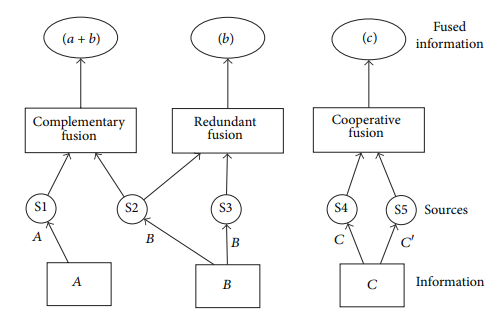
\includegraphics[width=0.8\textwidth]{classificacao_fusao_de_sensores.png}
					\label{fig:classificacao_fusao_de_sensores}
					\smallcaption{Fonte: Retirado de \textcite{castanedo2013review}}
				\end{figure}
			
			\subsubsection{Classificação em três níveis}
			
				A fusão de dados normalmente aborda três níveis de abstração: medidas, características e decisões. Essa maneira de classificar os diferentes métodos de fusão de sensores se baseia nessa ideia, dividindo-os em baixo, intermediário e alto nível, como é descrito a seguir \cite{castanedo2013review}.
			
				\begin{itemize}
					\item \textbf{Nível baixo:} também chamada de fusão de dados crus, essa categoria combina diferentes fontes de dados crus para produzir novos dados que espera-se que sejam mais informativos do que os de entrada.
					
					\item \textbf{Nível intermediário:} também chamada de fusão a nível de características, essa categoria combina diversos aspectos, como bordas, linhas, texturas ou posições em um mapa de características que pode ser utilizado para segmentação ou detecção.
					
					\item \textbf{Nível alto:} também chamada de fusão de decisões, essa categoria combina decisões de diversos especialistas para obter uma decisão ainda mais precisa. Normalmente métodos bayesianos são empregados neste nível.
					
					\item \textbf{Nível múltiplo:} esse nível aborda dados providenciados de diferentes níveis de abstração. Um exemplo é a união de uma medição com uma característica para obter uma decisão.
				\end{itemize}
				
				Segundo essa classificação, esse projeto utiliza uma fusão em baixo nível, visto que utiliza dados crus de sensores a fim de predizer a localização de um robô móvel, que é um dado mais informativo do que os dados de entrada.
			
			\subsubsection{Classificação baseada na entrada e saída do sistema}
			
				Esse sistema de classificação proposto por \textcite{dasarathy1997sensor} (por isso também chamado de modelo de Dasarathy) refinou o modelo de classificação em três níveis, dividindo as diferentes técnicas de fusão de sensores em 5 categorias baseado no nível de abstração dos dados de entrada e saída do sistema. As características das 5 categorias são resumidas de acordo com a natureza da entrada e os resultados de saída do processo de fusão \cite{li2021data, vakil2021survey}. 
				
				\begin{itemize}
					\item \textbf{Entrada de dados-Saída de dados (DAI-DAO):} é o tipo mais básico de fusão de dados, nele há o processo de entradas e saídas de dados crus, os resultados são tipicamente mais confiáveis e acurados. Nesse caso a fusão é conduzida imediatamente depois da coleta de dados dos sensores.
					
					\item \textbf{Entrada de dados-Saída de características (DAI-FEO):} nesse nível o processo de fusão emprega dados crus das fontes para extrair características ou aspectos que descrevem a entidade do ambiente.
					
					\item \textbf{Entrada de características-Saída de características (FEI-FEO):} nesse nível tanto a saída quanto a entrada dos dados do processo de fusão são características. Assim, o processo aborda um conjunto de aspectos a fim de melhorar, refinar ou obter novas características.
					
					\item \textbf{Entrada de características-Saída de decisões (FEI-DEO):} este nível recebe um conjunto de características e, a partir delas, fornece um conjunto de decisões como saída do sistema. A maior parte dos sistemas que realizam uma decisão baseada no recebimento de dados de sensores entram nessa categoria.
					
					\item \textbf{Entrada de decisões-Saída de decisões (DEI-DEO):} esse tipo de classificação é também conhecida como fusão de decisão, já que funde decisões de entrada para obtenção de melhores ou novas decisões.
				\end{itemize}
				
				A partir dessa classificação, pode-se dizer que a fusão de sensores desse projeto funcionou com entrada de dados e saída de dados, já que foram utilizados dados de posição, aceleração e velocidade para conseguir melhores dados de posição e orientação.
				
				A Figura \ref{fig:classificacao_2_fusao_de_sensores} representa claramente a diferença entre as cinco categorias de classificação proposta por \textcite{dasarathy1997sensor}. Já a Figura \ref{fig:classificacao_3_fusao_de_sensores} relaciona e mostra as diferenças entre os modelos de classificação em três níveis e Dasarathy.
			
				\begin{figure}[!htb]
					\centering
					\caption{Diagrama representando a diferença entre as fusões baseadas no nível de abstração dos dados.} 
					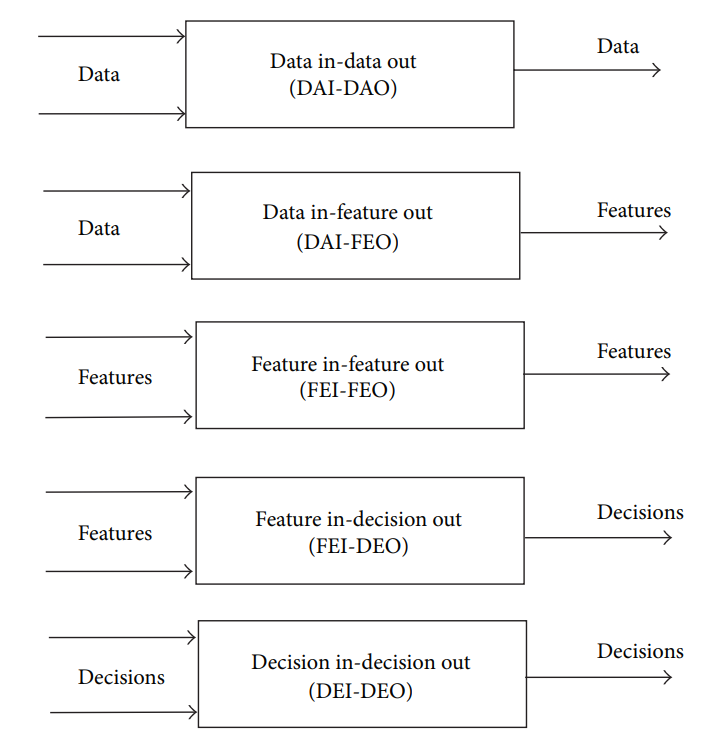
\includegraphics[width=0.6\textwidth]{classificacao_2_fusao_de_sensores.png}
					\label{fig:classificacao_2_fusao_de_sensores}
					\smallcaption{Fonte: Retirado de \textcite{castanedo2013review}}
				\end{figure}
			
				\begin{figure}[!htb]
					\centering
					\caption{Diagrama relacionando as classificações três níveis e Dasarathy.} 
					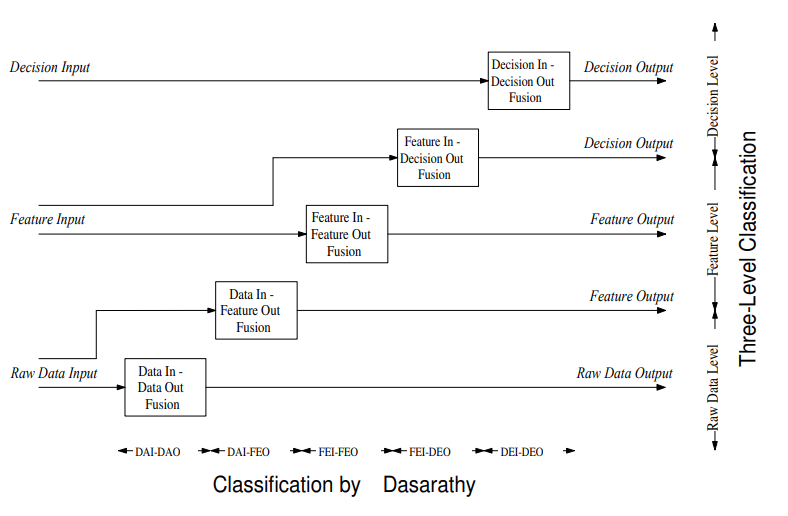
\includegraphics[width=0.8\textwidth]{classificacao_3_fusao_de_sensores.png}
					\label{fig:classificacao_3_fusao_de_sensores}
					\smallcaption{Fonte: Retirado de \textcite{elmenreich2002introduction}}
				\end{figure}
	
	\section{FILTRO DE KALMAN}
		
		Nesta seção serão abordados os conceitos teóricos necessários para entendimento do tão divulgado e utilizado filtro de Kalman. Nela, serão apresentadas suas equações, as premissas para desenvolvimento das equações, as etapas do algoritmo, assim como a apresentação do filtro de Kalman estendido, utilizado em situações cujo sistema e/ou medição são não-lineares. 
		
		No caso desse trabalho, o filtro de Kalman é o algoritmo utilizado para realizar a fusão de diferentes sensores a fim de estimar a localização de robôs móveis, por isso a importância da descrição detalhada do seu funcionamento ao longo dessa seção.
		
		\subsection{Utilização}
		
			O filtro de Kalman (\acrshort{kf}) foi inventado durante a década de 50 por Rudolph Emil Kalman como uma técnica para filtragem e predição em sistemas lineares. Desde então, por conta dos avanços na área de computação digital, o KF é objeto de extenso estudo e aplicações, particularmente na área de navegação autônoma ou assistida.
			
			O filtro de Kalman é um algoritmo que já foi utilizado em uma vasta gama de aplicações, principalmente na área de controle e na predição de sistemas dinâmicos, sendo a base para o desenvolvimento da teoria do controle moderno e processamento de sinais em tempo real. Nos dias de hoje, segundo \textcite{khodarahmi2023review}, o \glsxtrshort{kf} evoluiu de um simples estimador de estados ótimo e possui aplicações na automação, posicionamento, rastreamento de alvo, processamento de sinais, imagens digitais, sinais de voz e previsão de terremotos.
			
			Focando mais no campo da robótica, o filtro de Kalman é aplicado no rastreamento de trajetória, estimativa de posição para robôs manipuladores, SLAM (do inglês, \textit{Simultaneous Localization and Mapping}) e detecção de objetos \cite{urrea2021kalman}. Além de que sua flexibilidade permitiu a integração da informação de diferentes tipos de sensores e técnicas, tornando possível responder as questões fundamentais da navegação de robôs: "Onde estou?", "Para onde estou indo?" e "E como eu chego no meu destino?".
			
			Em suma, o filtro de Kalman é um conjunto de equações matemáticas que serve para estimar o estado de um sistema dinâmico linear com ruídos de tal maneira que a média do erro quadrático diminui de forma eficiente computacionalmente por ser um algoritmo recursivo. Ou seja, o \glsxtrshort{kf} precisa de pouca memória já que salva informação de estados passados, sendo adequado para problemas de tempo real e sistemas embarcados \cite{khodarahmi2023review}.
			
			Quando fala-se sobre o estado de um sistema, coloca-se um vetor $x$ que consiste de $n$ variáveis que descrevem importantes propriedades de um sistema. Um exemplo de estado é a pose de um robô, que consiste das coordenadas $x$ e $y$ e a orientação $\theta$ de um robô.
			
			Como colocado anteriormente, robôs normalmente utilizam uma grande quantidade de sensores, cada um deles provendo a posição do robô, mas também cada um sendo sujeito a erros ou falhas no funcionamento. Portanto, a obtenção da localização ótima de um robô móvel deve levar em conta a informação gerada por todos sensores. Segundo \textcite{siegwart2011introduction}, o filtro de Kalman é uma técnica poderosa para atingir essa fusão de sensores por ser eficiente ao representar a função de densidade probabilística da crença do robô e até das leituras individuais dos sensores, resultando num algoritmo de processamento de dados recursivo ótimo.
			
			Entretanto, segundo \textcite{phdthesisNegenborn}, o fato de que as variáveis de um estado podem conter ruídos e não serem diretamente observáveis dificultam a estimação do estado. O KF possui acesso às medições do sistema para poder realizar a estimativa do estado, estas medições estão linearmente relacionadas ao estado e estão corrompidas por ruídos. Caso as fontes desses ruídos possuírem uma distribuição gaussiana, a estimativa do KF é estatisticamente ótima para qualquer medida razoável de otimização.
			
			Também segundo \textcite{phdthesisNegenborn}, o KF processa todas medidas disponíveis de sensores para estimar o estado, tanto as medidas precisas quanto as imprecisas. Ele utiliza conhecimento do sistema e dinâmica dos sensores, descrição probabilística do próprio sistema e dos ruídos das medidas, e qualquer dado disponível sobre os valores iniciais do estado.
			
		\subsection{Premissas}
		
			A utilização do filtro de Kalman para predizer e corrigir a crença do estado presume a necessidade de um modelo tanto do sistema quanto das medições. O \acrshort{kf} assume uma descrição de sistema dinâmico linear do sistema que está estimando o estado. O sistema dinâmico pode ser corrompido por fontes de ruídos, os quais o \acrshort{kf} assume que podem ser modelados por distribuições independentes, brancas, média zero e gaussianas \cite{urrea2021kalman}.
			
			\subsubsection{Sistema dinâmico linear}
			
				Falando sobre o modelo do sistema, ele descreve como o verdadeiro estado do sistema evolui ao longo do tempo, utilizado pelo filtro para realizar predições sobre o estado. Basicamente, o \acrshort{kf} assume que o estado do sistema evolui de acordo com a Equação \eqref{eq:premissas_equacao_modelo_sistema}, onde o verdadeiro estado $x_k$ do sistema no tempo $k$ depende do estado um passo antes $x_{k-1}$ e algum ruído, a matriz $A$ tem tamanho $n \times n$ e relaciona os estados passado e atual, enquanto o vetor $w_{k-1}$ modela o ruído no sistema, adicionando os efeitos de influências não modeladas no estado \cite{urrea2021kalman}.
				
				\begin{equation}\label{eq:premissas_equacao_modelo_sistema}
					x_k = Ax_{k-1} + Bu_{k-1} + w_{k-1}
				\end{equation}
			
				O modelo de medição descreve como medições se relacionam com os estados. O filtro de Kalman necessita do modelo das medições a fim de corrigir a predição do estado quando uma medição está disponível. Basicamente, o \acrshort{kf} assume que as medições podem ser modeladas por um equação linear que relaciona o estado do sistema para uma medição, como a Equação \eqref{eq:premissas_equacao_medicoes}, em que $z_k$ depende linearmente do estado do sistema $x_k$, já a matriz H possui tamanho $m \times n$ e relaciona a medição com o estado, enquanto $v_k$ é o ruído nas medições \cite{khodarahmi2023review}.
				
				\begin{equation}\label{eq:premissas_equacao_medicoes}
					z_k = Hx_k + v_k
				\end{equation}
			
				Ambas Equações \eqref{eq:premissas_equacao_modelo_sistema} e \eqref{eq:premissas_equacao_medicoes} mostram que o estado $x_k$ no tempo $k$ não depende de todos os outros estados e medições dado $x_{k-1}$ e que a medição $z_k$ não depende de qualquer estado ou medida, o que torna o sistema um processo Markoviano.
			
			\subsubsection{Características do ruído}
				
				Uma característica necessária do ruído para o filtro de Kalman é a independência, que torna o cálculo envolvido na estimativa de estado mais fácil. De acordo com \textcite{phdthesisNegenborn} em geral é justo assumir que os ruídos no sistema e medição são independentes.
				
				Outra característica que simplifica a matemática envolvida no filtro de Kalman é o ruído branco, este tem poder em todas frequências do espectro e é completamente não correlacionado com ele mesmo em qualquer momento exceto o presente. Ou seja, os erros não se correlacionam pelo tempo, saber a quantidade de ruído neste momento não ajuda em predizer qual será a quantidade de ruído em outro momento.
				
				Uma terceira característica que é assumida é que o ruído possui média zero, o que implica que o erro no sistema e medição é aleatório. Um ruído aleatório significa que ele não é sistemático, ou seja, ele não possui um \textit{bias} constante, algumas horas ele é positivo, outras negativo, mas sempre média zero.
				
				A última característica importante que é assumida pelo filtro de Kalman é que o ruído é gaussiano, que é uma característica que lida com amplitude do ruído, colocando que a quantidade de ruído envolvida pode ser modelada por uma curva conforme a Figura \ref{fig:distribuicao_gaussiana}, em que o centro do gráfico representa a média $\mu$ dos valores, já a dispersão (ou largura) do gráfico é representada pelo desvio padrão $\sigma$ (ou pela variância, que é o desvio padrão elevado ao quadrado). Esta premissa é justificada ao assumir que os ruídos do sistema e medição são causados por diversas fontes pequenas de ruídos que, independente de suas distribuições, a soma delas será distribuída conforme uma gaussiana.
				
				\begin{figure}[!htb]
					\centering
					\caption{Exemplo de distribuição gaussiana.} 
					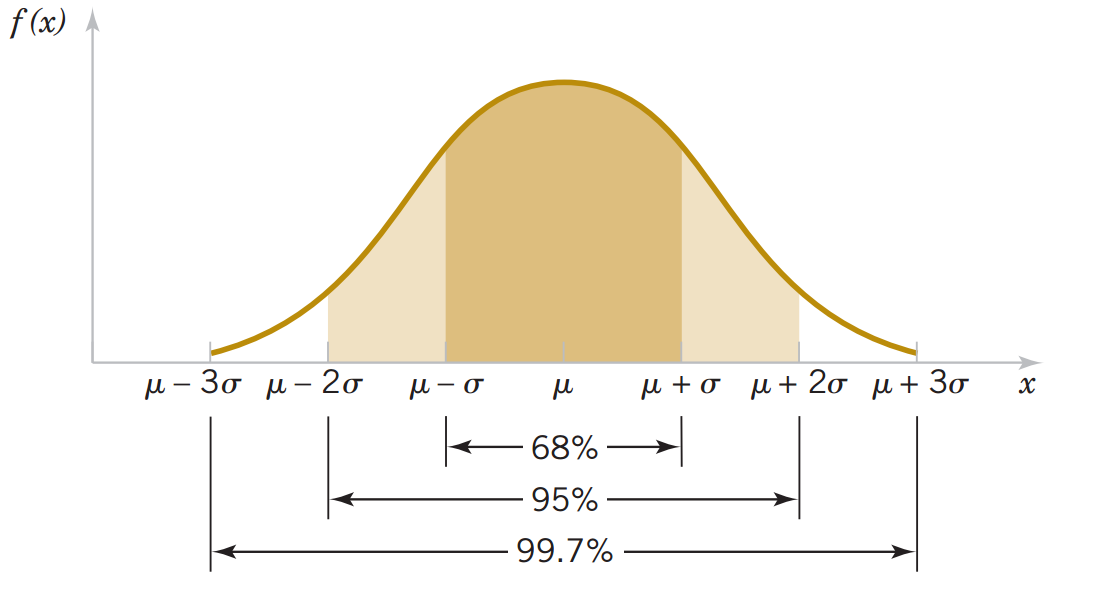
\includegraphics[width=0.6\textwidth]{distribuicao_gaussiana.png}
					\label{fig:distribuicao_gaussiana}
					\smallcaption{Fonte: Retirado de \textcite{normal_distribution}}
				\end{figure}
			
				Com as premissas da média zero e a distribuição gaussiana, os ruídos podem ser descritos de acordo com $N(\mu,\Sigma)$, que denota uma função gaussiana de média $\mu$ e covariância $\Sigma$.
		
		\subsubsection{Processo a ser estimado}
		
			O filtro de Kalman aborda o problema geral de tentar estimar o estado $x \in \mathbb{R}^n$ de um processo controlado em tempo discreto que é governado pela equação diferencial estocástica linear descrita pela Equação \eqref{eq:equacao_estado_sistema} com medição $z \in \mathbb{R}^m$, que é representada pela Equação \eqref{eq:equacao_medicao_sistema}. No caso, as variáveis aleatória $w_k$ e $v_k$ representam os ruídos do processo e das medições, respectivamente.
			
			\begin{equation} \label{eq:equacao_estado_sistema}
				x_k = Ax_{k-1} + Bu_{k-1} + w_{k-1}
			\end{equation}
		
			\begin{equation} \label{eq:equacao_medicao_sistema}
				z_k = Hx_k + v_k
			\end{equation}
		
			Assume-se que as variáveis $w_k$ e $v_k$ são independentes uma das outras, brancas, e com uma distribuição probabilística normal, segundo as probabilidades definidas na Equação \eqref{eq:equacao_probabilidade_variaveis_ruido}.
			
			\begin{equation} \label{eq:equacao_probabilidade_variaveis_ruido}
				\begin{split}
					p(w) &\sim N(0, Q) \\
					p(v) &\sim N(0, R)
				\end{split}
			\end{equation}
		
			Segundo \textcite{welch1995introduction}, a matriz de covariância do ruído do processo Q e a matriz de covariância do ruído das medições R podem variar a cada passo de tempo ou a cada medição, embora nesse caso seja considerado constante.
			
			A matriz A da Equação \eqref{eq:equacao_estado_sistema} possui tamanho $n \times n$ e relaciona o estado no passo de tempo anterior $k - 1$ com o estado no passo de tempo atual $k$ na ausência de uma função ou ruído de processo. Já a matriz B possui tamanho $n \times l$ e relaciona a entrada de controle $u \in \mathbb{R}^l$ ao estado $x$. A matriz H possui tamanho $m \times n$ na Equação \eqref{eq:equacao_medicao_sistema} e relaciona o estado com a medição $z_k$.
			
		\subsection{Equações} \label{sec:filtro_de_kalman_equacoes}
			
			De acordo com \textcite{khodarahmi2023review}, o filtro de Kalman estima um processo utilizando uma forma de controle por meio de feedback, nele o filtro estima o estado do processo em um dado instante e obtém feedbacks na forma de medições, no caso ruidosas. Como tal, as equações do filtro de Kalman podem ser divididas em dois grupos: as equações de atualização de tempo e as equações de atualização de medições. O primeiro grupo é responsável por projetar a frente no tempo as estimativas do estado atual e a covariância do erro para obter a estimativa a priori do próximo período de tempo. Já o segundo grupo é responsável pelo feedback, isto é, por incorporar uma nova medição na estimativa a priori a fim de obter uma melhor estimativa a posteriori.
			
			As equações de atualização no tempo podem ser chamadas como equações de predição, enquanto as equações de atualização de medição podem ser chamadas de equações de correção. Basicamente o algoritmo de estimativa final se assemelha com um algoritmo predição-correção para solução de problemas numéricos. A Figura \ref{fig:predicao_atualizacao_kalman} mostra o ciclo do filtro de Kalman, em que a predição projeta a estimativa do estado atual a frente no tempo, enquanto a correção ajusta a estimativa projetada por uma medição real naquele instante.
			
			\begin{figure}[!htb]
				\centering
				\caption{Ciclo do filtro de Kalman discreto.} 
				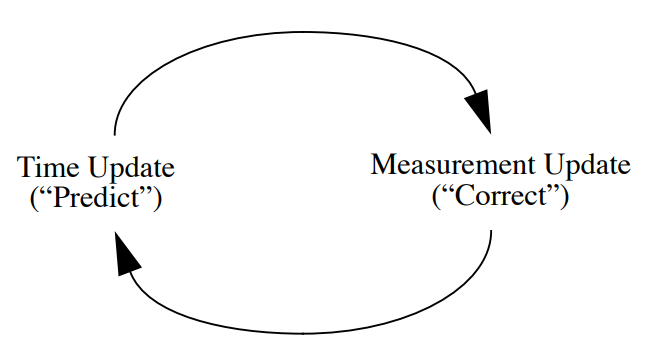
\includegraphics[width=0.6\textwidth]{predicao_atualizacao_kalman.png}
				\label{fig:predicao_atualizacao_kalman}
				\smallcaption{Fonte: Retirado de \textcite{welch1995introduction}}
			\end{figure}
			
			\subsubsection{Predição}
				A cada instante de tempo o sistema pode estar em um estado diferente. Portanto, o \acrshort{kf} calcula uma nova crença anterior a cada passo de tempo. As equações de predição (também chamada de atualização por tempo ou propagação) predizem o novo estado do sistema projetando à frente a crença mais recente, ou seja, calculando a crença $bel(x_k)$ a partir da crença do estado anterior $bel(x_{k-1})$. 
				
				No caso, de acordo com \textcite{thrun2002probabilistic}, $bel(x_k) = N(\hat{x}_{k}^{-},P_{k}^{-})$, em que a média $\hat{x}_{k}^{-}$ e a covariância $P_{k}^{-}$ são definidos segundo a Equação \eqref{eq:equacao_predicao_kf}. É importante destacar que a notação \^{} representa uma estimativa do estado, enquanto a notação $^-$ representa que a variável foi predita, ou seja, antes de incorporar a medição.
				
				\begin{equation} \label{eq:equacao_predicao_kf}
					\begin{split}
						&\hat{x}_{k}^{-} = A\hat{x}_{k-1} + Bu_{k} \\
						&P_{k}^{-} = AP_{k-1}A^{T} + Q_{k}					
					\end{split}
				\end{equation}
			
				O \acrshort{kf} calcula a estimativa de estado $\hat{x}_{k}^{-}$ baseado tanto na última estimativa de estado $\hat{x}_{k-1}$ quanto no modelo disponível do sistema. A melhor hipótese que o \acrshort{kf} pode fazer sobre o estado do sistema depois dele progredir um passo a frente no tempo é a melhor hipótese propagada pelo modelo que o \acrshort{kf} possui do sistema.
				
				Além disso, o filtro de Kalman também reconhece que a evolução do sistema está sujeita a ruídos e, assim, possui uma incerteza aumentada $P_{k}^{-}$ na estimativa do estado. O primeiro termo da covariância do erro $AP_{k-1}A^{T}$ propaga a incerteza da última estimativa à frente para a estimativa atual do estado. Já o segundo termo $Q_{k}$ é o ruído do sistema que corrompe o estado do sistema a cada passo de tempo.
			
			\subsubsection{Correção}
			
				As equações de correção (ou atualização da medição) lidam com as medições dos sensores. Elas são utilizadas apenas quando há a atualização da medição dos sensores. As medições providenciam informação direta sobre o estado atual do sistema. As equações desta etapa corrigem a previsão da crença mais recente ao incorporar a informação recebida das medições. Segundo \textcite{thrun2002probabilistic}, as equações dessa fase calculam a crença posterior $bel(x_k) = N(\hat{x}_{k},P_{k})$, em que $\hat{x}_{k}$ e $P_{k}$ são definidos segundo a Equação \eqref{eq:equacao_medicao_kf}.
				
				\begin{equation} \label{eq:equacao_medicao_kf}
					\begin{split}
						&\hat{x}_{k} = \hat{x}_{k}^{-} + K_{k}(z_k - H\hat{x}_{k}^{-}) \\
						&P_{k} = (I - K_kH)P_{k}^{-} \\
						&K_k =  P_{k}^{-}H^T(HP_{k}^{-}H^T + R_k)^{-1}
					\end{split}
				\end{equation}
			
				A nova crença posterior $\hat{x}_{k}$ é utilizada no próximo passo de tempo para calcular a predição de uma nova crença. A natureza recursiva do filtro de Kalman permite implementações práticas, já que nem todos os dados são necessários para estimar os estados.
				
				O filtro de Kalman calcula a estimativa do estado posterior combinando a predição da estimativa de estado com o ganho de Kalman $K_k$ vezes a diferença entre a medição $z_k$ e a previsão de medição $H\hat{x}_{k}^{-}$, chamada de inovação.
				
				O termo $H\hat{x}_{k}^{-}$ na Equação \eqref{eq:equacao_medicao_kf} é chamado de previsão de medição. Dadas a estimativa do estado anterior ${x}_{k}^{-}$ e a matriz de medições $H$ do modelo de medição na Equação \eqref{eq:equacao_medicao_sistema}, o filtro de Kalman prediz qual medição irá receber. Assim, denota-se a previsão de medição segundo a Equação \eqref{eq:previsao_de_medicao_kf}.
				
				\begin{equation} \label{eq:previsao_de_medicao_kf}
					\hat{z}_k = H\hat{x}_{k}^{-} + \hat{v}_k
				\end{equation}
			
				No caso, o ruído de medição $\hat{v}_k$ é zero e a previsão de medição é uma variável aleatória que segue uma distribuição gaussiana, podendo notar isso ao analisar que ela depende linearmente da estimativa anterior do estado $\hat{x}_{k}^{-}$ e do ruído de medição, sendo que ambos são variáveis aleatórias gaussianas. Logo, facilmente deriva-se que a predição de medida $\hat{z}_k$ segue a distribuição descrita na Equação \eqref{eq:distribuicao_predicao_medicao}.
				
				\begin{equation} \label{eq:distribuicao_predicao_medicao}
					\hat{z}_k = N_z( H\hat{x}_{k}^{-}, HP_{k}^{-}H^T + R_k)
				\end{equation}
			
				A diferença entre a medição $z_k$ e a medição prevista $x_{k}^{-}$ é chamada de inovação da medição ou $\tilde{z}_k$ residual. A inovação diz quanto uma medida prevista difere de uma medição real, sendo definida segundo a Equação \eqref{eq:equacao_inovacao_medicao}. Caso a inovação seja igual a zero, a medida prevista reflete exatamente a medição real, o que implica que o estado estimado com o qual a predição da medição foi realizada estava muito perto do verdadeiro estado que a medição foi feita. Entretanto, se existir uma diferença entre as medições prevista e observada, a estimativa do estado anterior precisa ser atualizada com um certo valor.
				
				\begin{equation} \label{eq:equacao_inovacao_medicao}
					\tilde{z}_k = z_k - \hat{z}_k
				\end{equation}
				
%				A inovação depende das variáveis $z_k$ e $\tilde{z}_k$. Sabe-se que a medição real $z_k$ é dada que não adiciona nenhuma incerteza à inovação. A incerteza na inovação depende apenas da incerteza na predição de medida $\tilde{z}_k$ e é, assim, distribuído de forma gaussiana, como é demonstrado na Equação \eqref{eq:distribuicao_gaussiana_medicao}.
%				
%				\begin{equation} \label{eq:distribuicao_gaussiana_medicao}
%					\begin{split}
%						\tilde{z}_k \sim N_z(\mu_{\tilde{z},k}, \Sigma_{\tilde{z},k}) \\
%						\mu_{\tilde{z},k} = z_k - \hat{z}_{k} \\
%						\Sigma_{\tilde{z},k} = HP_{k}^{-}H^T +R_k
%					\end{split}
%				\end{equation}
%			
%				Nota-se que se há incerteza na medição real (por conta de incerteza na extração de uma característica, por exemplo), então a incerteza na inovação deve aumentar. A distribuição da inovação dá uma ideia de espalhamento das inovações, dando uma ideia dos erros nas estimativas de medições.
				
				O fator $K_k$ na Equação \eqref{eq:equacao_medicao_kf} é chamado de ganho de Kalman (\glsxtrshort{kg}, do inglês \textit{Kalman Gain}), que é o fator que determina até que ponto a inovação deve ser levada em conta na estimativa de estado posterior. Isso é determinado ao olhar a incerteza relativa entre a estimativa de estado anterior e a inovação da medição, como descrito na Equação \eqref{eq:equacao_medicao_kf}.
				
				A fim de comparar a incerteza da estimativa do estado anterior no espaço de estados com a incerteza da inovação no espaço de medição, o \acrshort{kf} converte a incerteza no espaço de medição para o espaço de estados por meio da matriz $H^T$.
				
%				Quando a covariância do erro de medida $R_k$ se aproxima de zero, o \acrshort{kg} pesa mais para o lado da inovação, isto é, a inovação de medição $\tilde{z}_k$ é confiável para conter mais informações do que a estimativa do estado anterior, tal como descrito na Equação \eqref{eq:equacao_limite_ganho_kalman}. Ou seja, o \acrshort{kf} acredita menos no modelo do sistema e mais nas medições.
%				
%				\begin{equation} \label{eq:equacao_limite_ganho_kalman}
%					\lim_{R_k \rightarrow 0 }K_k = H^{-1}
%				\end{equation}
%			
%				Do contrário, quando a covariância do erro anterior $P^{-}_k$ se aproxima de zero, o \acrshort{kg} pesa menos para o lado do residual, isto é, quanto mais a covariância do erro anterior $P^{-}_k$ se aproxima de zero, menos a medição residual $\tilde{z}_k$ é levada em conta, como mostrado na Equação \eqref{eq:equacao_limite_ganho_kalman_2}. Ou seja, o \acrshort{kf} confia mais no modelo do sistema e menos nas medições.
%				
%				\begin{equation} \label{eq:equacao_limite_ganho_kalman_2}
%					\lim_{P^{-}_k \rightarrow 0 }K_k = 0
%				\end{equation}
%			
%				O filtro de Kalman também utiliza o ganho de Kalman para atualizar a incerteza que o próprio \acrshort{kf} possui na estimativa de estado posterior em ser o estado verdadeiro. Se o \acrshort{kg} está perto de $H^{-1}$ a inovação das medições é levada em conta quase completamente. Isso significa que o \acrshort{kf} confia que a inovação contém relativamente mais informação comparada com a estimativa de estado anterior. Isto resulta na diminuição máxima da incerteza do estado.
%				
%				Se as observações observam os valores de cada variável de estado diretamente e há uma grande quantidade de incerteza na estimativa de estado anterior relativa às medições, então o ganho de Kalman será perto de $H^{-1}$ e a estimativa do erro posterior estará próxima de zero. Isto vai levar ao \acrshort{kg} a não levar as próximas medições tanto em conta, já que a incerteza no estado é bem pequena, então o \acrshort{kg} também será. O tempo que leva até que o \acrshort{kf} leve novamente em consideração as inovações de forma significativa depende da quantidade de ruído do sistema adicionado na incerteza da estimativa de estado anterior a cada instante de tempo.
				
				Em resumo, o ciclo do filtro de Kalman pode ser entendido conforme o Algoritmo \ref{alg:kf_algoritmo}, em que há o detalhamento das Equações de cada um dos passos do \acrshort{kf}, a predição e correção. Já a Figura \ref{fig:exemplo_filtro_de_kalman_covariancias} representa um exemplo em uma dimensão de como o filtro de Kalman realiza a predição e correção em termos de média e covariância.
				
%				\begin{figure}[!htb]
%					\centering
%					\caption{Ciclo do filtro de Kalman discreto detalhado com as equações de cada passo.} 
%					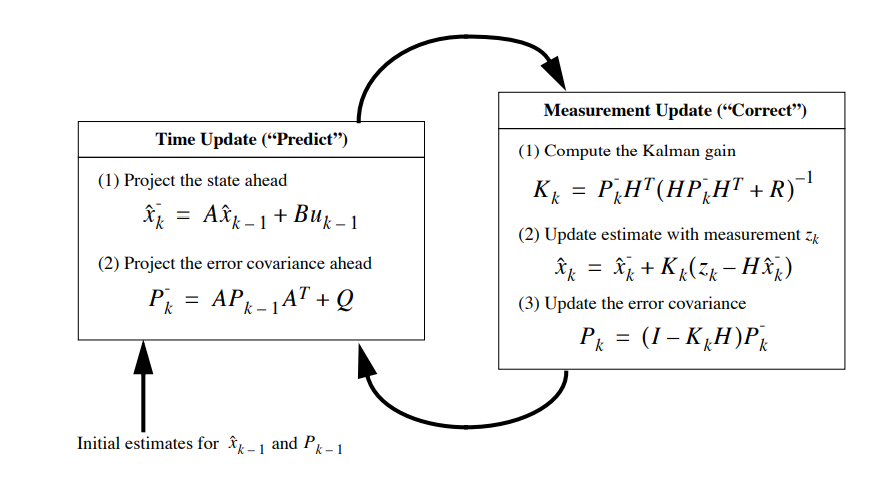
\includegraphics[width=0.8\textwidth]{ciclo_filtro_de_kalman_equacoes.png}
%					\label{fig:ciclo_filtro_de_kalman_equacoes}
%					\smallcaption{Fonte: Retirado de \textcite{welch1995introduction}}
%				\end{figure}

				\begin{algorithm}
					\Entrada{Estado anterior \(x_{k-1}\); Covariância anterior \(P_{k-1}\); Entrada de controle \(u_k\); Entrada de medição \(z_k\)}
					\Saida{Estado atual \(\hat{x_{k}}\); Covariância atual \(P_{k}\)}
					\Inicio{
						\(\hat{x}_{k}^{-} = A\hat{x}_{k-1} + Bu_{k}\) \\
						\(P_{k}^{-} = AP_{k-1}A^{T} + Q_{k}\) \\
						\Se{medição disponível}{
							\(K_k =  P_{k}^{-}H^T(HP_{k}^{-}H^T + R_k)^{-1}\) \\
							\(\hat{x}_{k} = \hat{x}_{k}^{-} + K_{k}(z_k - H\hat{x}_{k}^{-})\) \\
							\(P_{k} = (I - K_kH)P_{k}^{-}\) \\
						}
					}
					\Retorna{\(\hat{x_k}\), \(P_k\)}
					\caption{Filtro de Kalman linear}\label{alg:kf_algoritmo}
				\end{algorithm}
			
				\begin{figure}[!htb]
					\centering
					\caption{Exemplo de predição e atualização das covariâncias do filtro de Kalman.}
					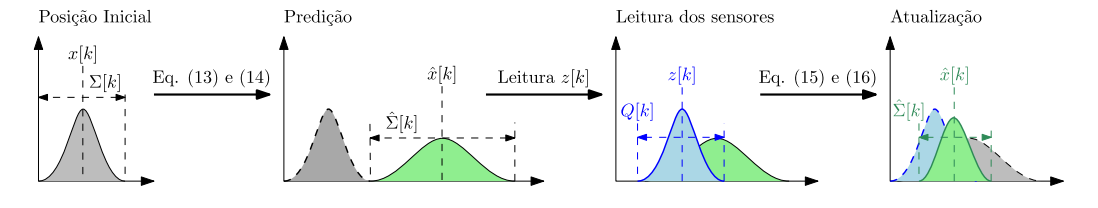
\includegraphics[width=0.9\textwidth]{exemplo_filtro_de_kalman.png}
					\label{fig:exemplo_filtro_de_kalman_covariancias}
					\smallcaption{Fonte: Retirado de \textcite{costaleonardo2023}}
				\end{figure}
		
		\section{FILTRO DE KALMAN ESTENDIDO}
			
			Para sua descrição, o filtro de Kalman possui algumas premissas, tal como a de que as observações são funções lineares do estados e que o próximo estado é uma função linear do estado anterior, o que é crucial para a correção do filtro \cite{thrun2002probabilistic}. Não só isso, para o desenvolvimento do \glsxtrshort{kf}, observa-se que qualquer transformação linear de uma variável aleatória gaussiana resulta em outra variável aleatória gaussiana. 
			
			Embora o filtro de Kalman tenha provado sua eficiência e qualidade ao longo dos anos com sua vasta utilização em diversas áreas, infelizmente sistemas mais complicados podem ser não-lineares \cite{khodarahmi2023review}. Por exemplo, um robô que se move com velocidade de translação e rotação constantes tipicamente realizam uma trajetória circular, que não pode ser descrita por uma transição de estado linear \cite{thrun2002probabilistic}.
			
			Logo, a fim de resolver o problema da linearidade para o filtro de Kalman, foi desenvolvida uma versão dele que leva em conta a não-linearidade dos sistemas, medições e ruídos, que é o filtro de Kalman estendido (\glsxtrshort{ekf}, do inglês).
			
			O \glsxtrshort{ekf} segue a mesma ideia do filtro de Kalman linear, isto é, com a separação nas etapas de predição, que projeta o sistema a frente para obter uma estimativa no próximo período de tempo, e correção, que incorpora uma nova medição na estimativa da predição a fim de obter uma melhor estimativa. A diferença entre ambos recai na particularidade de que o \glsxtrshort{ekf} utiliza séries de Taylor para linearizar o sistema não-linear.
			
			De acordo com \textcite{thrun2002probabilistic}, a ideia da linearização é aproximar uma função não-linear $g$ por uma função linear que é tangente a $g$ na média da gaussiana. Assim, projetar a gaussiana por meio dessa aproximação linear resulta em uma densidade gaussiana, como é demonstrado na Figura \ref{fig:ekf_linearizacao}. O autor coloca que a principal vantagem da linearização recai na sua eficiência.
			
			\begin{figure}[!htb]
				\centering
				\caption{Exemplo de predição e atualização das covariâncias do filtro de Kalman.}
				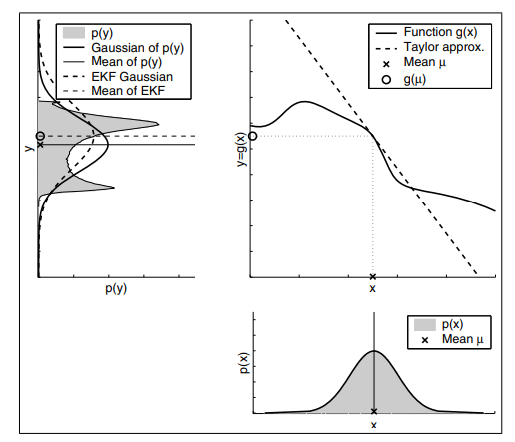
\includegraphics[width=0.7\textwidth]{figura_linearizacao_ekf.png}
				\label{fig:ekf_linearizacao}
				\smallcaption{Fonte: Retirado de \textcite{thrun2002probabilistic}}
			\end{figure}
			
			As predições lineares no filtro de Kalman são substituídas pelas generalizações não-lineares no filtro de Kalman estendido. Além de que o \glsxtrshort{ekf} utiliza de Jacobianas $G_k$ e $C_k$ ao invés das matrizes lineares do sistema $A_k$, $B_k$ e $H_k$ no \glsxtrshort{kf}.
			
			Assim, a etapa de predição no filtro de Kalman estendido é descrita conforme a Equação \eqref{eq:equacao_predicao_ekf}. É possível notar que a estimativa do estado é dada por uma função não-linear $f$ que depende do estado anterior $x_{k-1}$ e da entrada de controle naquele instante $u_{k}$. Além disso, como dito anteriormente, $G_{k}$ é a matriz Jacobiana com relação ao estado. No caso, uma matriz Jacobiana é formada pelas derivadas parciais de primeira ordem de uma função. A variável $P$ representa a covariância dos estados e $Q$ os ruídos do sistema.
			
			\begin{equation} \label{eq:equacao_predicao_ekf}
				\begin{split}
					&\hat{x}_{k}^{-} = f(x_{k-1}, u_{k}) \\
					&P_{k}^{-} = G_{k}P_{k-1}G_{k}^{T} + Q_{k} \\
					&G_{k} = \frac{\partial f(x_{k-1}, u_{k})}{\partial x_{k-1}} 
				\end{split}
			\end{equation}
			
			A etapa de correção no filtro de Kalman estendido é descrita conforme a Equação \eqref{eq:equacao_medicao_ekf}. No caso, a estimativa do sensor também é uma função não-linear. Assim, $C_k$ representa a matriz Jacobiana do sensor com relação ao estado, já $h(x_{k}^{-})$ representa a linearização do sensor. A variável $K$ representa o ganho de Kalman do sistema e $R$ representa os ruídos das medições.
			
			\begin{equation} \label{eq:equacao_medicao_ekf}
				\begin{split}
					&z_k = h(x_{k}) \\
					&\hat{x}_{k} = \hat{x}_{k}^{-} + K_{k}(z_k - h(x_{k}^{-})) \\
					&P_{k} = (I - K_{k}C_{k})P_{k}^{-} \\
					&K_k = P_{k}^{-}C_{k}^T(C_{k}P_{k}^{-}C_{k}^T + R_k)^{-1} \\
					&C_k = \frac{\partial h(x_k)}{\partial x_{k}}
				\end{split}
			\end{equation}
			
			As equações que representam o filtro de Kalman estendido podem ser entendidas em conjunto segundo o Algoritmo \ref{alg:ekf_algoritmo}.
			
			\begin{algorithm}
					\Entrada{Estado anterior \(x_{k-1}\); Covariância anterior \(P_{k-1}\); Entrada de controle \(u_k\); Entrada de medição \(z_k\)}
					\Saida{Estado atual \(\hat{x_{k}}\); Covariância atual \(P_{k}\)}
					\Inicio{
						\(\hat{x}_{k}^{-} = f(x_{k-1}, u_{k}) \) \\
						\(P_{k}^{-} = G_{k}P_{k-1}G_{k}^{T} + Q_{k} \) \\
						\Se{medição disponível}{
							\(K_k = P_{k}^{-}C_{k}^T(C_{k}P_{k}^{-}C_{k}^T + R_k)^{-1}\) \\
							\(\hat{x}_{k} = \hat{x}_{k}^{-} + K_{k}(z_k - h(x_{k}^{-}))\) \\
							\(P_{k} = (I - K_{k}C_{k})P_{k}^{-}\) \\
						}
					}
					\Retorna{\(\hat{x_k}\), \(P_k\)}
					\caption{Filtro de Kalman estendido}\label{alg:ekf_algoritmo}
			\end{algorithm}
			
\chapter{Trabalhos relacionados}\label{sec:trab_relacionados}
Diversos estudos foram realizados na área de localização de robôs móveis e estimativa de posição a fim de obter o conhecimento necessário para o desenvolvimento do projeto em questão. Entretanto, uma boa gama dos trabalhos encontrados utilizam robôs com uma dinâmica diferente de um robô omnidirecional da \textit{Small Size League} da RoboCup, como o modelo de duas rodas ou o modelo \textit{car-like}, ou também os estudos levam em conta diferentes sensores dos que são utilizados nesse projeto.

A seguir serão descritos os trabalhos relacionados nas áreas de fusão de sensores, estimativa de posição de robôs móveis e filtro de Kalman. Os termos utilizados na pesquisa dos trabalhos foram "\textit{position estimation}", "\textit{position estimation kalman filter}, "\textit{sensor fusion for position estimation}" e "\textit{position estimation sensor fusion}".

Em \textcite{eman2020mobile}, um filtro de Kalman estendido é utilizado para resolver o problema de localização de um robô móvel num ambiente \textit{indoor}. Os autores estudam a eficiência do filtro em três casos distintos na questão do ruído presente no sistema, que são: sem ruído, ruído Gaussiano, ruído não-Gaussiano.

Sobre o sistema, o modelo utilizado é de um robô de duas rodas, no qual as equações da cinemática do modelo estão descritas na Equação \eqref{eq:trab_relacionados_cinematica_1}, que os autores definem $(x, y)$ sendo a posição e $\theta$ a orientação do robô, $\mu$ a velocidade linear e $\omega$ a velocidade angular.

\begin{equation}\label{eq:trab_relacionados_cinematica_1}
	\begin{cases}
		\dot{x} = \mu \cos{\theta} \\
		\dot{y} = \mu \sin{\theta} \\
		\dot{\theta} = \omega
	\end{cases}
\end{equation}

A partir disso, utilizando aproximação de Taylor, a posição e a orientação do robô em qualquer momento futuro $k + 1$ são descritas segundo a Equação \eqref{eq:trab_relacionados_serie_taylor_1}, em que $T_s$ é o período de amostragem.

\begin{equation} \label{eq:trab_relacionados_serie_taylor_1}
	\begin{cases*}
		x(k+1) = x(k) + \mu(k)T_s\cos{(\theta(k))} \\
		y(k+1) = y(k) + \mu(k)T_s\sin{(\theta(k))} \\
		\theta(k+1) = \theta(k) + \omega(k)T_s
	\end{cases*}
\end{equation}

Já sobre o \glsxtrshort{ekf}, o autor determina que o vetor de estados a serem estimados $X$ e o vetor de controle $U$ são o que está definido na Equação \eqref{eq:trab_relacionados_vetor_estados_1}. Assim, as matrizes Jacobianas do sistema podem ser definidas conforme a Equação \eqref{eq:trab_relacionados_matrizes_jacobianas}.

\begin{equation}\label{eq:trab_relacionados_vetor_estados_1}
	\begin{cases}
		X = [x \quad y \quad \theta]^T \\
		U = [\mu \quad \omega]^T
	\end{cases}
\end{equation}

\begin{equation}\label{eq:trab_relacionados_matrizes_jacobianas}
	\begin{cases}
		A_k = \frac{\delta f(X_k, U_k)}{\delta X_k} = \begin{bmatrix}
			1 & 0 & -\mu(k)T_s\sin{(\theta(k))} \\
			0 & 1 & \mu(k)T_s\cos{(\theta(k))}  \\
			0 & 0 & 1
		\end{bmatrix} \\[30pt]
		
		H_k = \frac{\delta f(X_k, U_k)}{\delta X_k} = 
		\begin{bmatrix}
			1 & 0 & 0 \\
			0 & 1 & 0 \\
			0 & 0 & 1 
		\end{bmatrix}		
	\end{cases}
\end{equation}

Para realização dos testes, os códigos foram desenvolvidos utilizando MATLAB num cenário 2D, com $T_s$ sendo $0.1s$, $\mu$ sendo $5m/s$ e $\omega$ sendo $1rad/s$, além de que o vetor de estados inicial e a estimativa inicial são matrizes nulas. Como dito anteriormente, foram considerados 3 cenários de ruídos a fim de avaliar a atuação do \glsxtrshort{ekf}.

Os resultados mostraram que o \glsxtrshort{ekf} é uma boa ferramenta de estimativa para sinais ruidosos em todos os casos, embora os resultados tenham confirmado que o filtro funciona melhor no caso de ruídos Gaussianos comparado com ruídos não-Gaussianos. Essa conclusão é de suma importância para a realização desse trabalho, visto que os sinais dos sensores e do sistema deste projeto são assumidos como Gaussianos, além da importância do uso de diferentes tipos de ruídos para estudo.

Já em \textcite{korotaj2021kalman} é descrita a utilização de fusão de sensores para um sistema mecatrônico omnidirecional. As expressões são dadas para um filtro de Kalman linear discreto que junta dados de um magnetômetro e um giroscópio, e um filtro de Kalman estendido discreto que estima a posição e orientação da plataforma com dados de um acelerômetro também.

Sobre o sistema, a plataforma é composta de 2 níveis e possui 4 rodas acionadas para movimentação, cada uma acionada por um motor \glsxtrshort{dc} (do inglês, \textit{Direct Current}). Os sensores presentes na plataforma são um acelerômetro de 3 eixos, um giroscópio de 3 eixos e um magnetômetro.

A estimativa de estado é separada em duas partes, a primeira é a estimativa da orientação do sistema a partir da fusão do giroscópio e do magnetômetro utilizando \glsxtrshort{kf}. Essa orientação estimada é utilizada como uma observação melhorada da orientação para estimativa tanto da posição quanto da orientação na segunda parte por meio de um \glsxtrshort{ekf} discreto, já que o modelo cinemático da plataforma é não-linear, além de utilizar as velocidades de cada uma das rodas e as leituras do acelerômetro também.

Os resultados simulados da resposta de estimativa de estado mostraram satisfatórias acurácia e velocidade do procedimento de estimativa selecionado. Apesar das limitações do layout utilizado das rodas e imperfeições das ranhuras que conectam a roda o seu eixo do motor, os experimentos em tempo real confirmaram a eficiência da fusão de sensores.

O trabalho demonstrou uma maneira diferente da utilização do filtro de Kalman, já que ele é usado em um primeiro passo para estimar a orientação com os dados do magnetômetro para corrigir o erro da integração do giroscópio. Assim, a partir dessa estimativa, é possível utilizar o \glsxtrshort{ekf} para predizer tanto a posição quanto a orientação do veículo.

%	Em \textcite{sensorFusionKalmanFilter}, o autor utiliza um filtro de Kalman estendido para realizar a fusão da odometria com um sonar para navegação de um robô de duas rodas. Além disso, o autor faz a utilização de um sistema lógico adaptativo Fuzzy (\glsxtrshort{afls}, do inglês \textit{Adaptative Fuzzy Logic System}) a fim de evitar ruídos coloridos que podem levar o \glsxtrshort{ekf} a divergir fazendo um ganho adaptativo que leva em conta a inovação e a covariância da inovação.
%	
%	A fim de validar o modelo criado, os autores decidiram utilizar um caminho no formato de uma onde senoidal em um ambiente \textit{indoor}. Foram realizados três testes, o primeiro utilizando o \glsxtrshort{ekf} com apenas o sinal de medição da odometria (segundo o autor esse sensor possui um erro sistemático, o que não torna ele um ruído branco), os resultados mostraram que o \glsxtrshort{ekf} não foi o suficiente para correção do erro sistemático, já que houve apenas a filtragem do ruído branco. O segundo teste fez a uitlização do \glsxtrshort{ekf}, mas com adição da medição dos sonares e, então, nota-se que houve uma redução do erro sistemático, mas a movimentação do robô não era suave. O terceiro experimento foi utilizando o \glsxtrshort{afls} para adaptar o ganho do \glsxtrshort{ekf}, o que gerou uma suavidade maior na estimativa de posição.

Em \textcite{ismail2022soccer} é feito um estudo sobre a localização baseada em fusão de sensores de um robô de futebol da categoria \textit{Middle Size League} (\glsxtrshort{msl}) da \textit{RoboCup}. A \glsxtrshort{msl} é como se fosse uma categoria acima da \glsxtrshort{ssl} na questão de tamanho dos robôs, em que os robôs possuem carcaças maiores (de aproximadamente 1,30m X 30cm), além de que não há um sistema global de visão, ou seja, a visão deve estar embarcada em cada robô, assim cada robô deve estimar sua posição e orientação de forma automática e independente.

A maior parte dos robôs dessa categoria utilizam câmeras omnivisão, permitindo que os robôs tenham visão 360$^\circ$. A partir dessas imagens é utilizado filtro de partículas (\glsxtrshort{fp}) para estimar a posição e orientação do robô em campo, embora o filtro necessite de um processamento computacional pesado.

O sistema de fusão de sensores aplicada no trabalho pode ser visualizado na Figura \ref{fig:msl_sensor_fusion}, em que há a representação em um diagrama de blocos da fusão de sensores aplicada nos robôs da categoria \glsxtrshort{msl} em \textcite{ismail2022soccer}.

\begin{figure}[!htb]
	\centering
	\caption{Visão geral da fusão de sensores da odometria com o sistema de visão da categoria \glsxtrshort{msl}.} 
	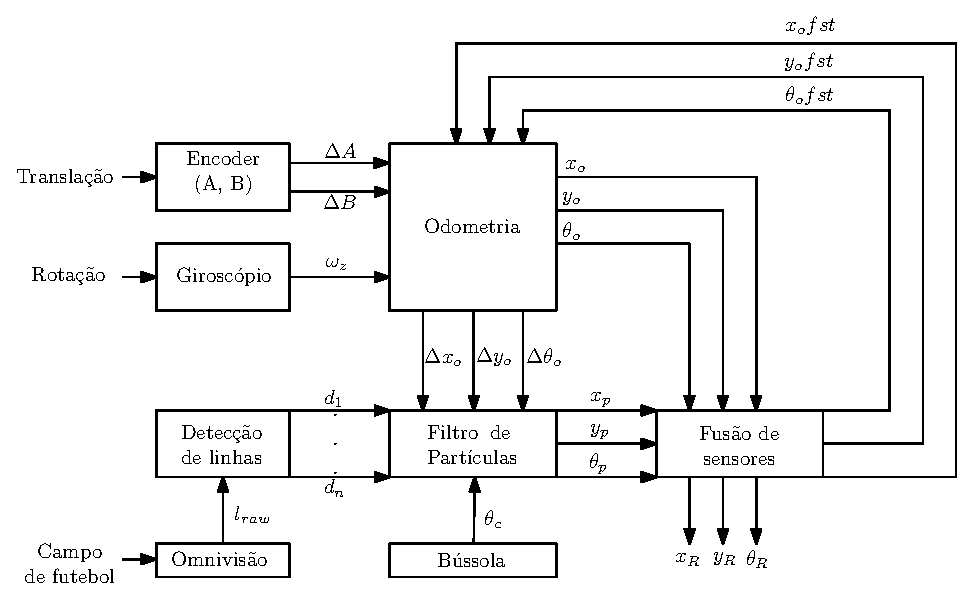
\includegraphics[width=0.8\textwidth]{msl_sensor_fusion.eps}
	\label{fig:msl_sensor_fusion}
	\smallcaption{Fonte: Retirado de \textcite{ismail2022soccer}}
\end{figure}

A partir da Figura \ref{fig:msl_sensor_fusion} é possível notar que o encoder e o giroscópio são utilizados para reconhecer a disposição do robô, sendo que são 2 encoders para detectar a translação e o giroscópio para detectar a rotação. Já a omnivisão detecta linhas brancas dentro do campo e, a partir das imagens cruas, há um processamento para gerar dados dessas linhas (i.e., cálculo da distância do robô até essas linhas por meio de regressão) antes de entrar no \glsxtrshort{fp}, que é ajudado por um bússola a fim de encontrar a posição .

%	Apesar da qualidade do filtro de partículas para estimar a localização dos robôs, os autores colocam que o algoritmo necessita conhecer o mapa do ambiente de trabalho para conseguir estimar a posição e orientação do robô nele.

A fusão de sensores atua combinando dados de posição e orientação do sistema de odometria e do \glsxtrshort{fp}. Os autores colocam que existem diferentes maneiras de realizar essa fusão (como comparação, junção, votação inteligente), mas no caso do trabalho são utilizados os métodos de fusão competitiva, onde os dados são tomados de forma independente, e complementar, em que há a utilização dos dados de ambos os sistemas de localização.

O teste realizado para validação do sistema de localização é o seguinte: o robô é movido manualmente para 20 coordenadas num campo de 9m x 6m, sendo que o movimento do robô é rastreado a fim de comparar com os dados de uma câmera global alocada em cima do campo. Depois de percorrer essas 20 coordenadas, são retirados a média, o desvio padrão do erro e o máximo erro dos sistemas de odometria, filtro de partículas e fusão de sensores.

A partir dos resultados, nota-se que no sistema de localização por odometria há um erro que cresce ao longo do tempo, enquanto para o \glsxtrshort{fp} e a fusão de sensores o erro não aumenta, enquanto a fusão dos dados acaba suavizando a saída quando comparado ao \glsxtrshort{fp}.

Além disso, um outro teste comparando ambos tipos de fusão de sensores foi realizado. O objetivo era movimentar o robô formando um zig-zag de maneira retangular. Os dados mostraram que o modo odometria é mais dominante, sendo que o sistema possui um tempo de resposta de aproximadamente 1.6ms para cada atualização de dados de localização.

Os autores concluem colocando que a fusão de sensores pode produzir dados ótimos ao combinar a odometria e a omnivisão com o \glsxtrshort{fp}. Os erros resultantes dos testes foram em x igual a 10.5 $\pm$ 7.8cm, em y igual a 7.6 $\pm$ 6.8cm e em $\theta$ igual a 1.9 $\pm$ 1.2$^\circ$. Esses resultados são melhores do que a utilização dos dados da odometria sozinhos, além de serem mais suaves do que o \glsxtrshort{fp} sozinho.

Este trabalho, por estar inserido na lógica do futebol de robôs, tem grande importância por utilizar um sistema de visão, mesmo que seja embarcado, diferente do sistema de visão da \glsxtrshort{ssl}. Além disso, o trabalho também compara duas maneiras de realizar a fusão de sensores com sensores que são semelhantes aos que foram utilizados nesse projeto.

Em \textcite{10.1007/978-3-642-54734-8_23} é realizado um estudo de fusão de sensores utilizando um sistema de visão e \glsxtrshort{imu} por meio de um filtro de Kalman de múltiplas taxas. No caso, a \glsxtrshort{imu} possui um processamento bem mais rápido do que o sistema de visão, além de que a taxa de atualização da primeira é constante enquanto o da segunda costuma ter oscilações.

No caso, o robô utilizado é do tipo direcional, sendo 4 rodas que são unidas em pares por 2 eixos. A \glsxtrshort{imu} é alocada no centro do robô, sendo que o giroscópio é alinhado com o eixo vertical.

Para lidar com as diferentes taxas de amostragem dos sistemas de visão e medição inercial é utilizado um \glsxtrshort{kf} discreto de múltiplas taxas, que segue a Equação \eqref{eq:kf_mult_rate}, em que Z é o vetor de estados $\begin{bmatrix} v_x & x & v_y & y & \theta \end{bmatrix}$, $Y_k$ é o vetor de valores medidos, $n_k$ e $w_k$ são ruídos. Já $A_k$ e $G_k$ são as matrizes do sistema. No caso, as matrizes $A_k$ e $G_k$ são descritas confrome a Equação \eqref{eq:kf_mult_rate_2}.

\begin{equation}\label{eq:kf_mult_rate}
	\begin{split}
		&Z_{k+1} = A_kZ_k + G_kn_k \\
		&Y_k = C_kZ_k + w_k
	\end{split}
\end{equation}

\begin{equation}\label{eq:kf_mult_rate_2}
	\begin{split}
		&A_k = \begin{bmatrix}
			1 & 0 & 0 & 0 & 0 \\
			\delta t_k & 1 & 0 & 0 & 0 \\
			0 & 0 & 1 & 0 & 0 \\
			0 & 0 & \delta t_k & 1 & 0\\
			0 & 0 & 0 & 0 & 0
		\end{bmatrix} \\
		&G_k = \begin{bmatrix}
			1 & 0 & 0 & \\
			0 & 0 & 0 \\
			0 & 1 & 0 \\
			0 & 0 & 0 \\ 
			0 & 0 & 1
		\end{bmatrix} \\
	\end{split}
\end{equation}

Os testes simulados foram realizados com o sistema inercial atualizando a uma taxa de 100Hz, enquanto o sistema de visão é simulado e fornece 2 medidas de posição por segundo. Os resultados mostraram que a trajetória do robô não apresenta um erro crescente ao longo do tempo, permanecendo abaixo de 3cm na maior parte do teste, sendo que o desvio aumenta quando o robô performa uma curva rápida com um raio pequeno, o que poderia ser mitigado com um sistema de visão mais rápido, segundo os autores.

Já nos resultados experimentais, o robô realizou uma trajetória com 4 seções em que se movia com velocidade linear de 10cm/s e uma velocidade angular de 0.2rad/s. As estimativas do filtro de Kalman eram calculadas a cada 25ms. Os resultados demonstraram uma boa estimativa da posição real sendo que, de acordo com os autores, a precisão e a taxa de amostragem se adequam para boa parte de aplicações de controle.

O trabalho traz informações importantes para fusão de sensores com diferentes taxas de atualização, principalmente por conta do uso de um sistema de visão, que normalmente possui um delay consideravelmente alto em relação aos outros sensores, como \glsxtrshort{imu} e encoder. Os autores colocam que a cada momento de fusão o conjunto de sensores disponíveis varia, então a Equação \eqref{eq:kf_mult_rate} leva em conta a taxa de atualização.

Continuando com aplicações na competição do futebol de robôs, em \textcite{aguiar2017kalman} é feito um estudo comparando o filtro de Kalman estendido, o filtro de Kalman \textit{unscented} (do inglês, \glsxtrshort{ukf}) e o filtro de Kalman linear para rastreamento de posição para a categoria IEEE \textit{Very Small Size}, que é uma categoria com robôs menores que a \glsxtrshort{ssl}, já que os robôs devem caber num cubo de $7.5cm$ de lado.

Os robôs da categoria, em suma, são diferenciais, que possuem 2 motores acoplados em 2 rodas normalmente. Os autores colocam que para o rastreamento da posição podem ser utilizados 2 modelos estocásticos para um robô desse tipo, cada um com uma representação de estados diferente. 

O primeiro modelo é chamado de modelo \textit{unicycle}, em que o estado é dado por $x_k = \begin{bmatrix}
	x_k & y_k & \theta_k & v_k & \omega_k \end{bmatrix}^T$. No caso, os três primeiros são as coordenadas e orientação de um ponto fixo entre as rodas do robô em relação a um \textit{frame} de referência. No problema de rastreamento do robô oponente não se tem acesso às entradas de controle, mas a formulação do estado e a cinemática do robô são suficientes para extrair as estimativas da velocidade. Isso pode ser observado na Equação \eqref{eq:differential_equation_vsss_1}. É possível notar que as acelerações linear e angular são modeladas como um vetor aleatório Gaussiano com covariância $Q$.

\begin{equation} \label{eq:differential_equation_vsss_1}
	\begin{bmatrix}
		\dot{x}\\ \dot{y}\\ \dot{\theta}\\ \dot{v}\\ \dot{\omega}
	\end{bmatrix} = 
	\begin{bmatrix}
		v \times \cos \theta\\ v \times \cos \theta\\ \omega\\ 0\\ 0
	\end{bmatrix} + 
	\begin{bmatrix}
		0 & 0\\ 0 & 0\\ 0 & 0\\ 1 & 0\\ 0 & 1
	\end{bmatrix}
	\begin{bmatrix}
		w_a\\ w_{\alpha}
	\end{bmatrix}
\end{equation}

Já o modelo de observação é dado pelo sistema de visão, também posicionado acima do campo, provendo observações de posição e orientação. Entretanto, esses dados são ruidosos, assumidos aditivos e Gaussiano com covariância $R$, como é possível ver na Equação \eqref{eq:differential_equation_vsss_2}.

\begin{equation}\label{eq:differential_equation_vsss_2}
	z_k = 
	\begin{bmatrix}
		x_k \\ y_k \\ \theta_k
	\end{bmatrix} + 
	\begin{bmatrix}
		v_{x,k} \\ v_{y,k} \\ v_{\theta,k}
	\end{bmatrix}
\end{equation}

O segundo modelo é chamado de dupla integração, que é demonstrado na Equação \eqref{eq:differential_equation_vsss_3}. No caso, o estado do robô é $x_k = \begin{bmatrix} x_k & y_k & v_{x,k} & v_{y,k} \end{bmatrix}^T$ e o modelo de observação é obtido conforme a Equação \eqref{eq:differential_equation_vsss_4}. Na categoria VSS, pode não ser possível extrair de maneira fácil a orientação do oponente a partir do sistema de visão, já que o sistema de cores não é unificado, diferente da categoria \glsxtrshort{ssl}.

\begin{equation}\label{eq:differential_equation_vsss_3}
	\begin{bmatrix}
		x_k \\ y_k \\ v_{x,k} \\ v_{y,k}
	\end{bmatrix} = 
	\begin{bmatrix}
		1 & 0 & T & 0 \\
		0 & 1 & 0 & T \\
		0 & 0 & 1 & 0 \\
		0 & 0 & 0 & 1
	\end{bmatrix}
	\begin{bmatrix}
		x_{k-1} \\ y_{k-1} \\ v_{x,k-1} \\ v_{y,k-1}
	\end{bmatrix} + 
	\begin{bmatrix}
		\frac{T^{2}}{2} & 0 \\
		0 & \frac{T^{2}}{2} \\
		T & 0 \\
		0 & T
	\end{bmatrix}
	\begin{bmatrix}
		w_{a,x} \\
		w_{a,y}
	\end{bmatrix}
\end{equation}

\begin{equation}\label{eq:differential_equation_vsss_4}
	z_k = 
	\begin{bmatrix}
		x_k \\ y_k
	\end{bmatrix} + 
	\begin{bmatrix}
		v_{x,k} \\ v_{y,k}
	\end{bmatrix}
\end{equation}

Para validar as técnicas de rastreamento foram realizados testes com os robôs reais e na simulação. Os testes reais foram realizados em um campo da categoria VSS e foram extraídos as posições cartesianas e a orientação providas pelo sistema de visão.

Os dados reais mostraram que o \glsxtrshort{ekf} e o \glsxtrshort{ukf} obtiveram resultados iguais, indicando que não há necessidade da utilização de uma técnica mais complexa como a segunda, já que o modelo do VSS não é um sistema que representa grandes não-linearidades, portanto o \glsxtrshort{ekf} seria preferível por conta da simplicidade e custo computacional. Além disso, os autores colocam que com o modelo \textit{unicycle} é possível alcançar uma estimativa mais completa do estado por incluir a orientação e velocidade angular do robô.

Já para a simulação, com o modelo de dupla integração utilizando o filtro de Kalman linear, apesar da baixa precisão para representar a dinâmica de um robô diferencial, os autores colocam que a performance de estimativa foi quase a mesma em relação ao \glsxtrshort{ekf} e \glsxtrshort{ukf} com o modelo \textit{unicycle}, visto que o \glsxtrshort{ekf} apresentou um erro quadrático médio apenas 1.5\% menor que o \glsxtrshort{kf} para estimativa de velocidade. Isso mostra também que o modelo consegue estimar com sucesso a velocidade no caso em que não se possui a orientação do robô.

Este trabalho é mais um inserido na realidade do futebol de robôs e numa categoria tão dinâmica quanto a \glsxtrshort{ssl}. Além disso, o autor mostra duas maneiras possíveis para representar o modelo dinâmico de um sistema, mesmo que os robôs dessa categoria sejam diferenciais.

Em \textcite{10333060} é feito um estudo para atingir um posicionamento acurado de robôs inteligentes para agricultura por meio da integração de um GPS e sensores de odometria de baixo custo, justamente para que seja acessível aos pequenos e médios agricultores, utilizando o \glsxtrshort{ekf} para conseguir essa integração.

Para realizar a etapa de predição do \glsxtrshort{ekf} os autores definem os estados como sendo os erros na solução de navegação utilizando odometria. No caso, os estados são o erro na orientação do robô pela odometria, os erros nas medições da posição norte e leste da odometria, o desvio associado ao raio das rodas direita e esquerda do robô, o erro no tempo de recepção do sinal do GPS e o desvio do GPS. O processo do modelo é estabelecido pelas equações que governam a evolução dos erros de estado da odometria ao longo do tempo.

Já a etapa de atualização é dividida a partir da topologia utilizada. Como nesse trabalho não haverá a utilização do sensor GPS como atualização do \glsxtrshort{ekf}, dessa etapa basta falar que na topologia fracamente acoplada a inovação da medição é determinada como a diferença entre a posição cartesiana fixa e centrada na Terra medida pelo GPS e a estimativa correspondente da odometria. Já na topologia fortemente acoplada a inovação da medição é calculada como a diferença entre as pseudo-distâncias medidas pela antena receptora do GPS para todos satélites em vista e a solução de navegação odométrica.

O trabalho demonstrou bons resultados, com uma melhoria significativa da precisão e acurácia do robô no que diz respeito às estimativas de posição e orientação, com melhorias que podem chegar à 97\% comparadas com os dados tanto da navegação utilizando odometria somente quanto os dados utilizando só a navegação por GPS.

Os autores concluem que, apesar dos resultados positivos alcançados no trabalho, o sistema de navegação odométrica auxiliada por GPS não alcançou as especificações de acurácia de posicionamento exigidas pela norma SAE J2945 \cite{sae2016board}.

Apesar dos resultados não serem satisfatórios para os autores por não cumprirem o determinado pela norma especificada, o modo que a etapa de predição é descrita no trabalho é uma ideia diferente que pode ser utilizada neste trabalho.

Já em \textcite{9233826} é realizado o teste de uma estratégia diferente para utilização de filtros em um robô omnidirecional com 4 rodas. No caso, é utilizada uma estratégia multi-filtro em que um \glsxtrshort{kf} estima a velocidade da roda a partir da dinâmica do motor e tem como medidas a leitura de velocidade de um encoder e o valor de corrente no motor, além de um \glsxtrshort{ekf} e um filtro suave de estrutura variável (\glsxtrshort{fsev}) para estimativa do estado do robô.

Os testes conduzidos buscaram realizar diferentes combinações e encontrar a melhor, isto é, utilizando ou não o \glsxtrshort{kf} e, em seguida, utilizando ou não um dos outros 2 filtros para estimativa do robô. As simulações foram conduzidas utilizando MATLAB, apesar de que as constantes físicas do motor foram conseguidas experimentalmente por meio de um osciloscópio, um multímetro e um gerador de ondas.

Os resultados mostraram que apenas a utilização do \glsxtrshort{kf} nas rodas melhorou a precisão da estimativa em relação a utilização de nenhum filtro (erro médio quadrático de 10.02cm para 9.28cm no eixo X, por exemplo). Já a utilização de um filtro para estimativa do robô, mesmo sem um filtro para as rodas, acabou dobrando a precisão da estimativa, sendo que o \glsxtrshort{fsev} se mostrou ligeiramente mais acurado (4.63cm de erro médio quadrático para ambos no eixo X). Já a utilização de ambos em conjunto aumenta a precisão duplamente, gerando um erro médio quadrático menor que 2cm.

O trabalho demonstra a qualidade da utilização do filtro de Kalman para predição do estado do robô, além de mostrar uma maneira interessante para estimar a velocidade das rodas do veículo a partir do modelo do motor, mostrando que a junção de ambos traz resultados melhores estimando o estado atual.

A partir dos trabalhos observados, é notório que há uma lacuna no que diz respeito a comparação dos sensores normalmente utilizados em projetos de robótica para sistemas de localização, principalmente em aplicações relacionadas a futebol de robôs, sendo os únicos descritos nessa Seção os trabalhos de \textcite{aguiar2017kalman} e também \cite{ismail2022soccer}, que descrevem o desenvolvimento de um sistema de localização baseado em fusão de sensores, mas fazem outras comparações, como o método de fusão, ao invés de comparar diferentes sensores.

%	Já em \cite{rigatos2010extended}, uma comparação entre a utilização do \glsxtrshort{ekf} e do filtro de partículas (\glsxtrshort{fp}) para controle de movimentação de robôs móveis foi estudada. No caso, o autor coloca a necessidade de assumir que os ruídos de medição são gaussianos no \glsxtrshort{ekf}, enquanto o \glsxtrshort{fp} não necessita de nenhuma premissa para funcionar.
%	
%	Um modelo simplificado de um robô \textit{car-like} foi utilizado para realizar os testes propostos, para uma estimativa mais precisa são utilizados sonares e odometria da roda. No caso, foram utilizados cinco cenários que propunham observar conceitos diferentes nos testes. O primeiro cenário foi um linha reta no plano 2D, o segundo um círculo, o terceiro um caminho com formato de infinito ($\inf$), o quarto é praticamente o mesmo que o terceiro, mas com um círculo adicional no percurso, já o último é um caso de uma baliza paralela, a fim de obter resultados para a indústria automotiva.
%	
%	Os resultados dos diversos testes mostraram que o \glsxtrshort{fp} foi superior ao \glsxtrshort{ekf} em termos de acurácia da estimativa do vetor de estados e robustez ao ruído de medição. Entretanto, a performance do \glsxtrshort{fp} depende da quantidade de partículas, no caso foram utilizadas 1000 para os testes, e da inicialização delas. É possível notar que quanto mais partículas melhor a estimativa, mas o gasto compputacional também cresce bastante.
%	
%	Em \textcite{santini1997trajectory} os autores abordam também o problema da estimativa de posição e orientação de robôs móveis. No caso, são utilizados encoders conectados no eixo dos motores para um período curto de tempo, enquanto para limitar o erro crescente na posição e orientação desses sensores é utilizado um sensor externo baseado num cinto de sensores ultrassom. Para realizar a fusão dos sensores foi utilizado um \glsxtrshort{kf}.
%	
%	No caso, o autor definiu o vetor de estados do sistema como mostra a Equação \eqref{eq:trab_relacionados_modelo_1}, em que $x_k$ e $y_k$ são as coordenadas da posição cartesiana do ponto médio do segmento que conecta as rodas (centro de trajetória), enquanto $\alpha_k$ é o ângulo de orientação do robô, ambos com respeito à um sistema fixo de referência.
%	\begin{equation} \label{eq:trab_relacionados_modelo_1}
	%	X_k = (x_k, y_k, \alpha_k)^T
	%	\end{equation}
%	
%	O veículo de testes nesse caso foi um robô diferencial, em que a realização de curvas e manobras é realizada pela diferenciação da velocidade angular de cada roda. O cenário de teste foi um quadrado de $2$\gls{metros} de lado. O primeiro teste foi utilizar o \glsxtrshort{kf} apenas para estimativa da trajetória real do robô, sendo executado depois de cada movimentação elementar, como transladar e rotacionar. O segundo teste foi utilizando o sensor externo, o que melhorou consideravelmente, já que o erro absoluto de posição nunca ultrapassou $10cm$ e o erro de orientação ficou abaixo de $5^\circ$, enquanto o algoritmo interno baseado nos encoders apresentou um erro de $100cm$ e $40^\circ$.
			
\chapter{Metodologia}\label{sec:metodologia}

	Neste capítulo serão apresentados o domínio de teste do projeto proposto, os testes a serem realizados, como os sensores foram combinados, a calibração dos sensores e quais métricas foram analisadas para avaliação dos testes propostos.
	
	\section{DOMÍNIO DE TESTES} \label{sec:dominio_de_testes}
	
		Neste trabalho foi utilizado o domínio de teste da categoria \glsxtrshort{ssl} de futebol de robôs da RoboCup \cite{RoboCup}, descrito na Seção \ref{sec:small_size_league}. Nele, as combinações de sensores foram testadas e comparadas. Para a realização dos testes propostos, foi utilizado o campo de futebol do laboratório da equipe RoboFEI, que possui 4,3 X 3,6m, o que possibilita uma boa estimativa da movimentação do robô em um campo oficial da competição.
		
		O que torna a \acrshort{ssl} um interessante campo de teste para as combinações dos sensores são algumas características dos robôs e das partidas, como:
		
		\begin{itemize}
			\item \textbf{Velocidade alta dos robôs:} A dinamicidade das partidas se dá muito por conta da alta velocidade atingida pelos robôs, sendo necessário um bom sistema de controle de posição, o que requer um estimador de posição utilizando sensores além das câmeras da liga;
			
			\item \textbf{Altas penalidades para colisões:} as regras da competição punem severamente os times que causam muitas colisões, podendo levar a diversos cartões amarelos (um robô deve ficar fora do campo por 2 minutos), e até cartões vermelhos (o robô é expulso pelo resto da partida);
			
			\item \textbf{Alta precisão necessária para realização de jogadas:} por conta do pequeno tamanho tanto dos robôs e da bolinha, para realizar jogadas rápidas que evitem a chegada de robôs adversários, faz-se necessário uma alta precisão de posicionamento dos robôs.
		\end{itemize}
		
		Sobre o robô utilizado na equipe RoboFEI, os sensores giroscópio e acelerômetro estão presentes na placa de desenvolvimento STM32F411E-Disco \cite{datasheet_micro}, que é a placa onde está alocado o microcontrolador do robô. É possível observar uma imagem deste componente na Figura \ref{fig:stm32f411}. Esta placa fica alocada numa placa eletrônica chamada de principal, que também contém os \textit{drivers} de ativação dos motores do robô e o módulo de comunicação via rádio frequência.
		
		\begin{figure}[!htb]
			\centering
			\caption{Placa de desenvolvimento STM32F411E-Disco utilizada.}
			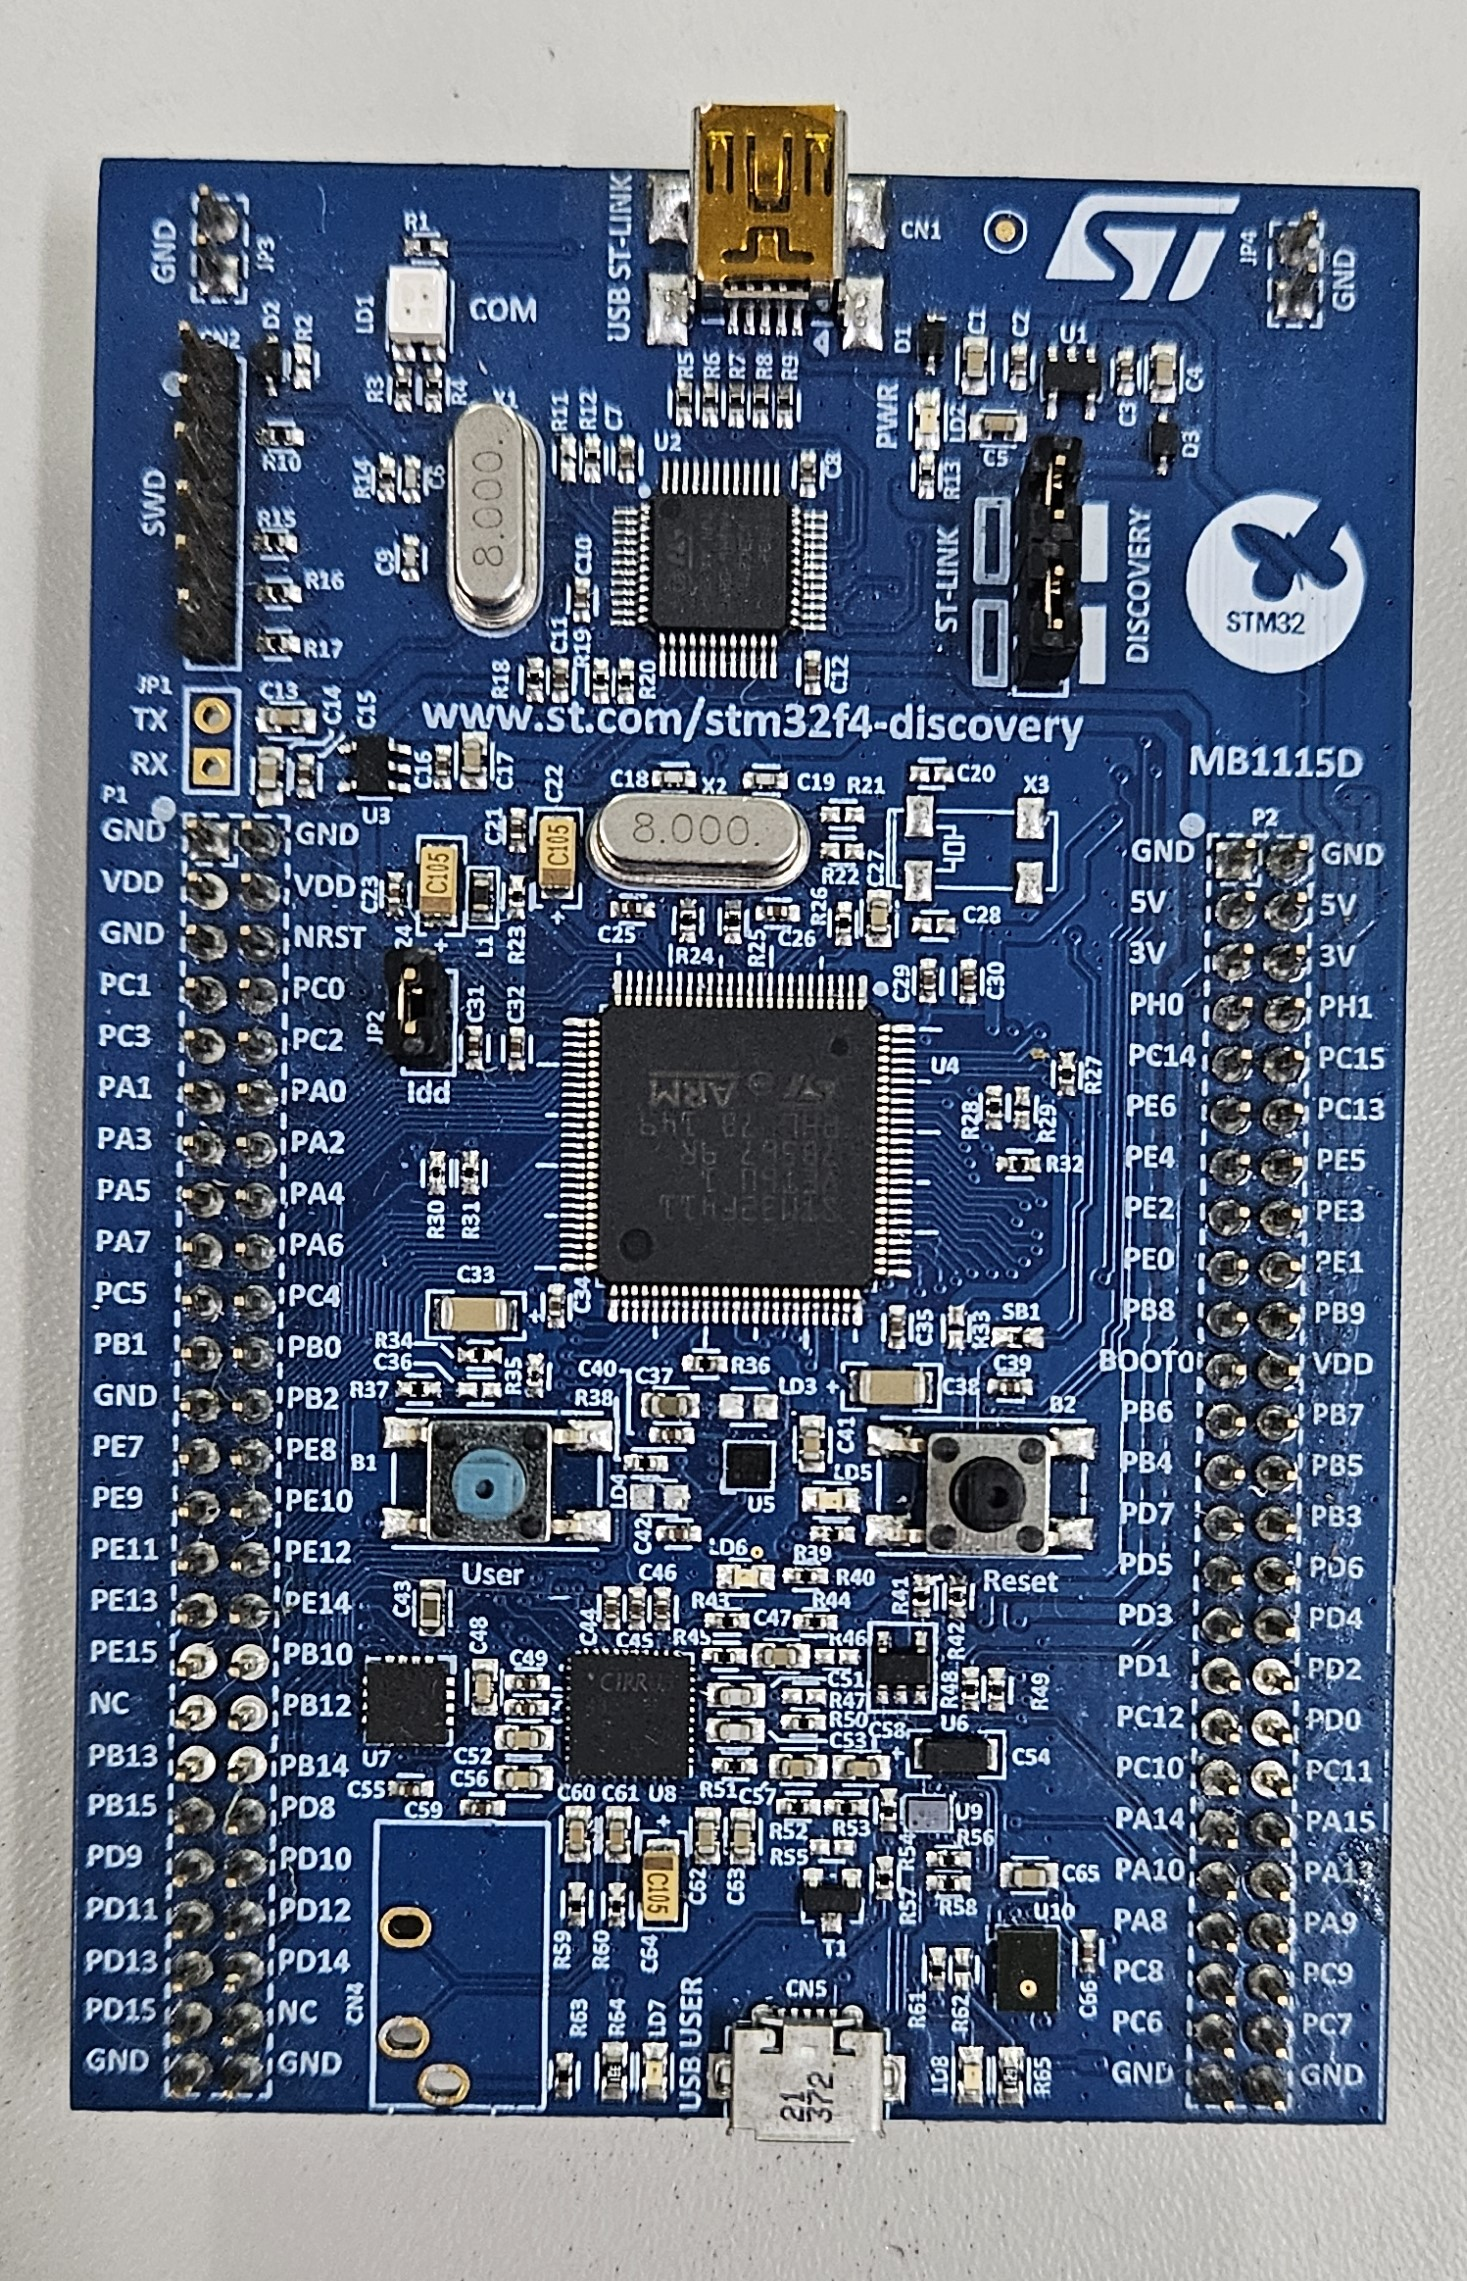
\includegraphics[width=0.5\textwidth]{stm32f411.jpg}
			\label{fig:stm32f411}
			\smallcaption{Fonte: Autor}
		\end{figure}
		
	\section{COMBINAÇÃO DOS SENSORES}\label{sec:metodologia_comb_sensores}
	
		Nesta seção serão definidos os sensores a serem utilizados e como eles foram combinados para realizar a predição e correção do filtro de Kalman.
		
		Os sensores utilizados nos testes são os descritos ao longo da Seção \ref{sec:sensores}, que são: IMU (Giroscópio + Acelerômetro), encoders, sistema de câmeras utilizado na \acrshort{ssl}, além do modelo cinemático do robô omnidirecional (apresentado na Seção \ref{sec:small_size_league}). Eles foram combinados entre as etapas de predição e correção a fim de encontrar a melhor configuração para realizar a estimativa de posição utilizando \glsxtrlong{ekf}, como é descrito na Tabela \ref{tbl:combinacao_sensores}.
		
		\begin{table*}[!htb]
			\centering
			\caption{Combinações dos sensores na predição e correção do Filtro de Kalman.}
			\label{tbl:combinacao_sensores}
			\begin{tabular}{|c|c|c|}
				\hline
				\textbf{Teste}   & \textbf{Predição} & \textbf{Correção} \\ \hline
				Cenário 1 		 & Modelo do sistema & Câmera   		 \\ \hline
				Cenário 2 		 & Modelo do sistema & Encoders 		 \\ \hline
				Cenário 3 		 & Modelo do sistema & \acrshort{imu} 	 \\ \hline
				Cenário 4 		 & \acrshort{imu}    & Câmera   		 \\ \hline
				Cenário 5 		 & \acrshort{imu}    & Encoders 		 \\ \hline
				Cenário 6 		 & Encoders          & Câmera   		 \\ \hline
				Cenário 7 		 & Encoders          & \acrshort{imu} 	 \\ \hline
				Cenário 8 		 & - 			 	 & Câmeras 			 \\ \hline
			\end{tabular}
			\smallcaption{Fonte: o Autor}
		\end{table*}
		
		No caso, os três primeiros cenários foram realizados utilizando o modelo cinemático do sistema na fase de predição, variando qual sensor era utilizado na fase de correção. Estes primeiros cenários serviram como uma introdução para o desenvolvimento do filtro de Kalman. No caso, o modelo cinemático do sistema leva em conta o comando de velocidade enviado para o robô da categoria \glsxtrshort{ssl} (ver Equação \eqref{eq:modelo_sistema_ssl} na Seção \ref{sec:small_size_league}). Os dois próximos cenários foram realizados com a \glsxtrshort{imu} na fase de predição, enquanto na fase de correção foram utilizados os outros dois sensores, respectivamente. Os dois cenários seguintes tiveram a mesma ideia dos testes 4 e 5, mas na fase de predição foram utilizados os encoders e na fase de correção os outros dois sensores. Já o cenário 8 é o sistema de localização atual da equipe, que utiliza apenas os dados vindos do sistema de câmeras, ou seja, não há uma fusão de sensores propriamente dita, e serve como comparação para os outros cenários.
		
%	\section{Calibração dos sensores} \label{sec:metodologia_calibracao}
%	
%		Como descrito na Seção \ref{sec:calibracao_sensores}, há a necessidade da calibração dos sensores giroscópio e acelerômetro presentes neste estudo. Toda a calibração será realizada com a placa eletrônica posicionada no robô, visto que posteriormente a ideia é realizar uma calibração individual dos sensores de cada um dos robôs.
%		
%		Assim, a primeira calibração a ser descrita é a do acelerômetro, que utiliza do método de \textcite{menezes2020triaxial}. No caso, serão tomadas amostras da aceleração nos 3 eixos em 9 posições diferentes para realização do método. Basicamente, a ideia é pegar amostras nas posições em que há os valores máximo e mínimo de aceleração em cada um dos eixos, e mais 3 posições em que o robô permanece em equilíbrio em cima de uma roda por vez. Em cada uma das posições serão lidas 4000 amostras em cada um dos eixos e, assim, será feita a média delas para cada um deles.
%		
%		Já para o giroscópio, a ideia é realizar a calibração em uma só posição, diferente do giroscópio. Para isso serão tomadas 30000 amostras de velocidade angular nos 3 eixos e, assim, será feita a média dessas amostras.
%		
%		Para validar a calibração de ambos os sensores, serão tomadas 10000 amostras nos 3 eixos antes e depois da calibração e a comparação será feita utilizando um gráfico do tipo \textit{box plot}. A ideia é que, para o giroscópio, em todos os eixos a média dos dados fique bem próxima de zero, tal como para o acelerômetro nos eixos X e Y, enquanto para o Z espera-se que fique em torno de 9.81$m/s^{2}$.
		
	\section{Implementação}
	
		Esta seção descreve a visão geral da implementação dos algoritmos deste trabalho, isto é, a linguagem utilizada para programá-los, o hardware utilizado e o fluxo geral do sistema de localização proposto.
		
		Em relação à linguagem de programação, para codificar os algoritmos de fusão de sensores no microcontrolador descrito na Seção \ref{sec:dominio_de_testes} foi utilizada linguagem C. A biblioteca CMSIS-DSP foi usada principalmente para auxiliar nos cálculos matriciais necessários nas equações do \glsxtrshort{ekf}, assim como para auxílio em cálculos que envolvam trigonometria \cite{cmsis_dsp}.
		
		O hardware utilizado no trabalho pode ser dividido em dois: o que é interno ao robô, e o que é externo ao robô. Internamente ao robô têm-se os sensores, que foram descritos na Seção \ref{sec:sensores}, além do microcontrolador utilizado para cálculo de fusão de sensores para localização de maneira embarcada. De modo externo ao robô deve-se considerar o notebook que é utilizado tanto para recebimento dos dados vindos do sistema de câmeras da categoria, mas também para cálculo da trajetória do robô em campo e para registro de dados a fim de análise dos resultados obtidos com os algoritmos. As especificações técnicas do notebook estão descritas na Tabela \ref{tbl:especificacoes_notebook}.
		
		\begin{table*}[!htb]
			\centering
			\caption{Especificações de hardware do notebook.}
			\label{tbl:especificacoes_notebook}
			\begin{tabular}{c c}
				\hline
				Sistema Operacional & Ubuntu 22.04.5 LTS x86\textunderscore64  \\ \hline
				CPU 				& Intel i7-7700HQ CPU @ 2.80GHz \\ \hline
				GPU 				& NVIDIA Geforce MX150 \\ \hline
				Memória RAM			& 16GB \\ \hline
			\end{tabular}
			\smallcaption{Fonte: o Autor}
		\end{table*}
	
		Além disso, as câmeras utilizadas pelo SSL-Vision para detecção dos robôs utilizando o padrão colorido em cima deles são as seguintes:
		
		\begin{itemize}
			\item Stingray F046C \cite{stingray_f046c} + Lente Tamron 12VM412ASIR
			\item Logitech BRIO 4K UHD \cite{logitech_brio}
		\end{itemize}
		
		Durante os testes, a transferência dos dados processados pelo SSL-Vision para o robô é feita via rádio-frequência, que a equipe já utiliza para enviar outros comandos para o robô, como velocidades locais, ativação do sistema de chute e acionamento do sistema de drible. Além disso, o \textit{feedback} das informações do robô para avaliação das combinações e dos sensores é transmitida a partir do robô para o computador central via rádio-frequência.
		
		O transceptor utilizado para comunicação entre a estação do rádio conectada ao computador da equipe e o robô é o módulo nRF24L01, que no caso opera numa frequência de 2.4GHz e necessita de poucos componentes para ser projetado como um sistema de rádio \cite{datasheet_nrf24}. O módulo é configurado e operado via \glsxtrshort{spi} acessando o mapa de registradores que servem para configurar o componente.
		
		O computador que roda a estratégia da equipe faz a formatação do pacote a ser enviado via rádio para o robô, sendo que o pacote pode ter um comprimento máximo de 32 bytes por conta da limitação do próprio nRF24L01. Assim, o pacote é transmitido para o transceptor por meio de comunicação serial via USB e, em seguida, o pacote é enviado para o robô, que verifica se o pacote pertence a ele pelo ID que é transmitido. O tamanho do pacote acaba sendo um gargalo tanto para o envio quanto para o recebimento das informações, visto que há outras informações que são transmitidas via rádio, como as velocidades linear, angular e do sistema de drible, ID do robô e tipo de chute (já que o robô pode fazer chutes retos ou "cavadinhas"), além da posição do robô em campo.
		
		As posições lidas e transmitidas para os robôs vindas do sistema global de câmeras da liga necessitam de 2 bytes cada, totalizando assim 6 bytes para transmissão dessas informações ao robô. Isto porque apenas 1 byte não é suficiente para transferir esses dados, já que seriam apenas 256 possibilidades ($2^8$ pela quantidade de bits num byte) e, por exemplo, a posição linear em X do robô pode ser de $\pm$4500mm, totalizando 9000 posições, logo 65536 possibilidades ($2^{16}$ utilizando 2 bytes) já é o suficiente.
		
		O diagrama geral do funcionamento do sistema de localização por fusão de sensores de forma embarcada ao robô pode ser observado na Figura \ref{fig:diagrama_implementacao}. Nela, é possível entender de maneira clara a diferença entre o que é calculado no computador central da equipe (recebimento dos dados do SSL-Vision e cálculo das velocidades locais desejadas) e o que é feito no microcontrolador do robô (recebimento dos dados do computador central, implementação dos sensores e cálculo da fusão de sensores).
		
		\begin{figure}[!htb]
			\centering
			\caption{Diagrama de implementação da fusão de sensores para localização.}
			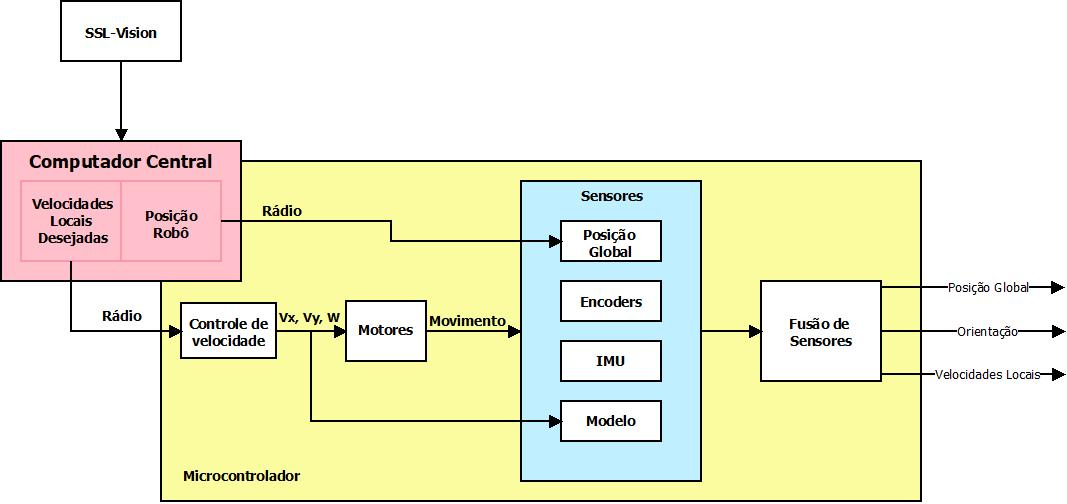
\includegraphics[width=1.00\textwidth]{diagrama_fluxo_implementacao.jpeg}
			\label{fig:diagrama_implementacao}
			\smallcaption{Fonte: Autor}
		\end{figure}
	
	\section{\textit{Ground Truth}}\label{sec:metodologia_ground_truth}
	
	O \textit{ground truth} é parte determinante desse projeto, visto a necessidade de comparar o sistema de localização desenvolvido com a posição real do robô em campo. Por conta disso, um sistema para calcular a posição real do robô foi desenvolvido utilizando dois LiDARs a fim de encontrar o formato arredondado dos robôs da categoria \glsxtrshort{ssl}.
	
	A Seção \ref{sec:resultados_ground_truth} traz o método desenvolvido em detalhes, assim como os resultados obtidos em comparação ao sistema de câmeras da categoria \glsxtrshort{ssl}, mas também em relação à medição manual utilizando uma trena.
	
	O sistema roda em conjunto ao recebimento dos dados e ao cálculo de trajetória do robô no notebook descrito na Tabela \ref{tbl:especificacoes_notebook}. Para performar a detecção, foram utilizados os lasers RPLIDAR A1 \cite{rplidar_a1} e RPLIDAR S2 \cite{rplidar_s2}, os modos de operação deles estão descritos na Tabela \ref{tbl:especificacoes_laser}. Além disso, ambos os sensores operaram com frequência de 10Hz.
	
	\begin{table*}[!htb]
		\centering
		\caption{Especificações dos LiDARs utilizados.}
		\label{tbl:especificacoes_laser}
		\begin{tabular}{|c|c|c|c|}
			\hline
			Sensor 				& Princípio 		& Modo de operação 	& Pontos capturados\\ \hline
			RPLIDAR A1			& Triangulação 		& Boost 			& 787 \\ \hline
			RPLIDAR S2 			& Time-of-Flight 	& Standard		    & 1612 \\ \hline
		\end{tabular}
		\smallcaption{Fonte: o Autor}
	\end{table*}

	Os LiDARs foram posicionados no meio de cada um dos gols a fim de obter uma melhor detecção, visto que o laser A1 tem um alcance máximo de 6 metros, e o erro de detecção aumenta gradualmente com a distância. Uma representação da posição dos lasers (pontos pretos), posição das câmeras (pontos azuis) e do robô pode ser vista na Figura \ref{fig:representacao_teste_lidar}.
	
	\begin{figure}[!htb]
		\centering
		\caption{Representação do posicionamento dos lasers em campo.}
		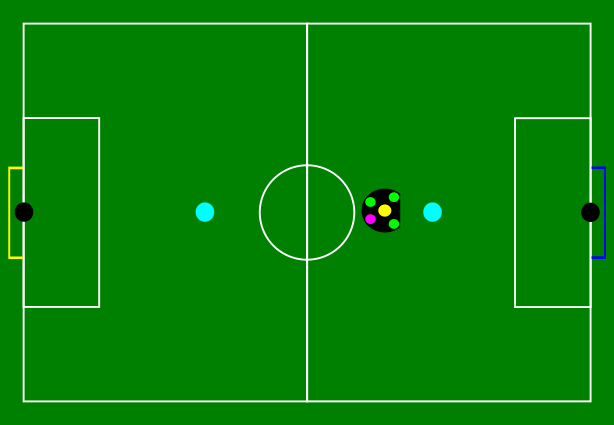
\includegraphics[width=0.80\textwidth]{representacao_teste_lidar_cameras.png}
		\label{fig:representacao_teste_lidar}
		\smallcaption{Fonte: Autor}
	\end{figure}

	Apesar de os LiDARs estarem posicionados aproximadamente numa mesma altura, é importante ressaltar que por conta da modulação da frequência do sinal enviado por cada um deles durante a varredura realizada, além do próprio funcionamento rotativo da varredura, que faz a janela de interferência ser uma fração de segundo, não há interferência entre ambos os LiDARs.
	
	\section{Sensores inerciais}
	
	Diferente dos dados das câmeras, os dados dos outros sensores são todos processados no microcontrolador embarcado no robô. Como dito nas Seções \ref{sec:sensores_giroscopio} e \ref{sec:sensores_acelerometro}, o acelerômetro e o giroscópio já estão presentes na placa de desenvolvimento utilizada no hardware do robô da equipe RoboFEI (Figura \ref{fig:stm32f411}), o que facilita para aquisição dos dados do sensor.
	
	\subsection{Acelerômetro}
	
	Como colocado na Seção \ref{sec:sensores_acelerometro}, os registradores do componente LSM303AGR podem ser acessados por meio das interfaces seriais \glsxtrshort{i2c} ou \glsxtrshort{spi}. No caso deste projeto, essa comunicação é realizada via \glsxtrshort{i2c}, onde o LSM303AGR é o escravo e o microcontrolador é o mestre.
	
	A biblioteca para obtenção dos dados do acelerômetro é disponibilizada pela própria desenvolvedora \cite{accelero_repository}. Sua utilização facilita a aquisição de dados, visto que a classe já possui métodos para inicialização do componente, filtragem passa-alta e leitura dos valores de aceleração do sensor, sendo necessária a escolha de alguns parâmetros de configuração, como frequência de saída de dados, escala e resolução.
	
	O sensor foi configurado com uma frequência de saída de 400Hz para que os dados a serem utilizados para estimativa de posição sejam atualizados de forma rápida. Já a escala escolhida, que define os limites do sensor, foi de $\pm2g$, já que as acelerações de um robô da categoria \glsxtrshort{ssl} não são maiores do que esse limite. Além disso, o sensor foi operado no modo de energia normal, o que permite uma saída de dados de até 10 bits. O componente possui outros dois modos, o de baixo consumo que produz uma saída de até 8 bits, e o de alta resolução, que produz uma saída de até 12 bits, porém a questão energética e/ou da resolução não são gargalos do projeto.
	
	\subsubsection{Calibração}
	
	Após a configuração do acelerômetro conforme explicação anterior, decidiu-se colher algumas amostras de dados do sensor. A Figura \ref{fig:dados_acelerometro_errado} apresenta os dados de 10000 amostras adquiridas do acelerômetro numa mesa plana com a placa em repouso, no caso foram extraídos dados dos três eixos, além do valor do módulo da aceleração, que no caso deve ser o valor da gravidade. O eixo vertical do gráfico representa a aceleração em $m/s^2$. Na Tabela \ref{tab:acelerometro_antes_calibracao} é possível observar alguns outros dados estatísticos das amostras do acelerômetro antes da calibração do sensor.
	
	\begin{figure}[!htb]
		\centering
		\caption{10000 amostras dos dados do acelerômetro antes da calibração.}
		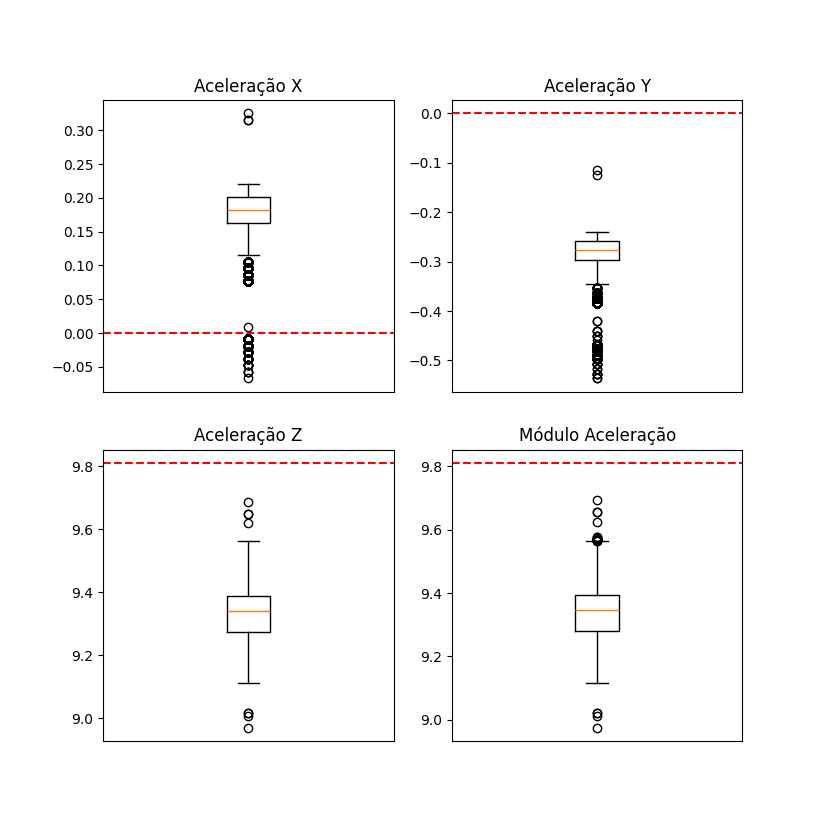
\includegraphics[width=0.7\textwidth]{dados_acelerometro_errados.png}
		\label{fig:dados_acelerometro_errado}
		\smallcaption{Fonte: Autor}
		\smallcaption{Legenda: o tracejado em vermelho representa a medida esperada em cada um dos eixos e também do módulo da aceleração.}
	\end{figure}
	
	\begin{table}[!htb]
		\centering
		\caption{Análise estatística dos dados do acelerômetro antes da calibração.}\label{tab:acelerometro_antes_calibracao}
		\begin{tabular}{|c|c|c|c|}
			\hline
			Dados & Média & Desvio Padrão ($\sigma$) & Variância ($\sigma^2$) \\ \hline
			\small Aceleração X & 0.169561  & 0.054271 & 0.002945 \\ \hline
			\small Aceleração Y & -0.294967 & 0.060317 & 0.003638 \\ \hline
			\small Aceleração Z & 9.327501  & 0.091915 & 0.008450 \\ \hline			
		\end{tabular}
	\end{table}
	
	A partir da Figura \ref{fig:dados_acelerometro_errado}, é nítido que as amostras estão longe das medidas esperadas, como uma diferença de quase 0.5$m/s^2$ no módulo geral, por exemplo. Além disso, a partir da Tabela \ref{tab:acelerometro_antes_calibracao} é possível notar também a média do valor da aceleração em Z, que é um valor bem distante do esperado. Essa grande diferença invalida a utilização do acelerômetro, mostrando a necessidade de uma calibração prévia do sensor.
	
	A calibração do acelerômetro, como descrito na Seção \ref{sec:calibracao_acelerometro}, é realizada pelo chamado método da esfera e é necessária a aquisição de 4000 amostras do sensor em 9 posições diferentes, sendo que em cada uma dessas posições é realizada a média das amostras tomadas, o que no caso são pontos utilizados para encontrar os desvios do acelerômetro. A Figura \ref{fig:dados_esfera_certo} mostra a esfera corrigida cujo raio é o valor da gravidade e o centro são os desvios do sensor, enquanto os pontos são as médias de cada uma das posições de calibração.
	
	\begin{figure}[!htb]
		\centering
		\caption{Esfera de calibração do acelerômetro.}
		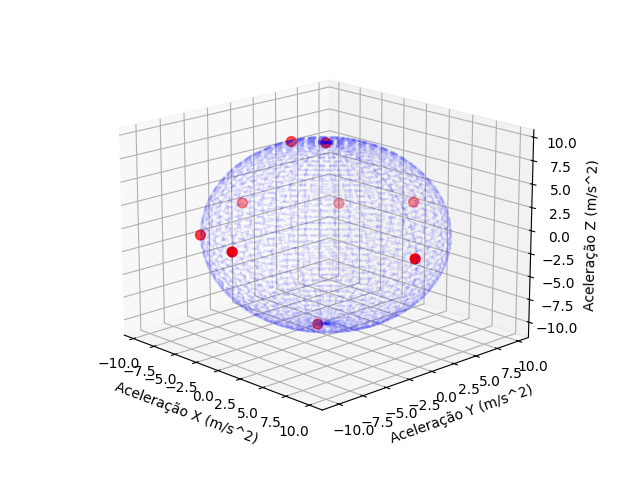
\includegraphics[width=0.8\textwidth]{dados_esfera_correto.png}
		\label{fig:dados_esfera_certo}
		\smallcaption{Fonte: Autor}
	\end{figure}
	
	Nota-se que os pontos estão bem em cima da esfera, o que demonstra êxito da calibração. Além do mais, na Figura \ref{fig:dados_acelerometro_certos} é possível observar os dados dos 3 eixos e do módulo desses valores das 10000 amostras (o eixo vertical do gráfico representa a aceleração em $m/s^2$) captadas depois da calibração e realizadas nas mesmas condições em que as amostras antes da calibração foram captadas. Além do mais, na Tabela \ref{tab:acelerometro_depois_calibracao} é possível notar algumas outras medidas das amostras colhidas depois da calibração.
	
	\begin{figure}[!htb]
		\centering
		\caption{10000 amostras dos dados do acelerômetro depois da calibração.}
		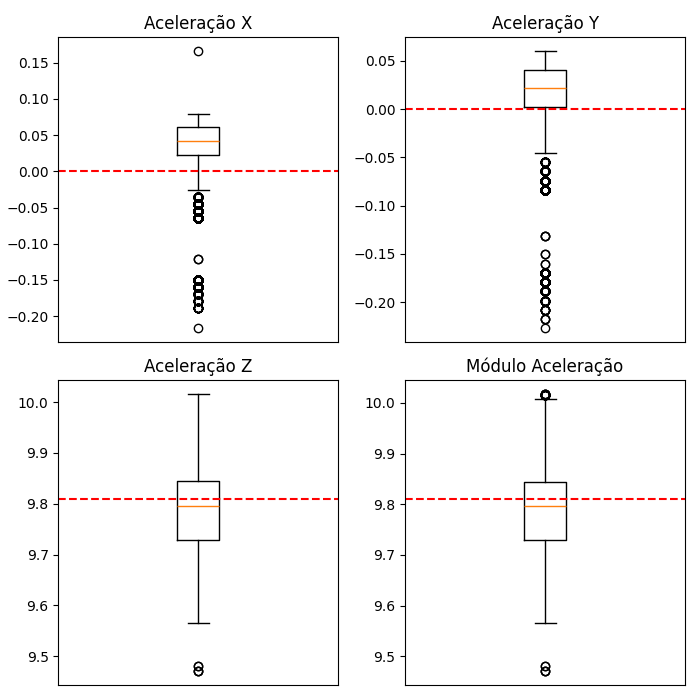
\includegraphics[width=0.7\textwidth]{dados_acelerometro_certos.png}
		\label{fig:dados_acelerometro_certos}
		\smallcaption{Fonte: Autor}
		\smallcaption{Legenda: o tracejado em vermelho representa a medida esperada em cada um dos eixos e também do módulo da aceleração.}
	\end{figure}
	
	\begin{table}[!htb]
		\centering
		\caption{Análise estatística dos dados do acelerômetro depois da calibração.}\label{tab:acelerometro_depois_calibracao}
		\begin{tabular}{|c|c|c|c|}
			\hline
			Dados & Média & Desvio Padrão ($\sigma$) & Variância ($\sigma^2$) \\ \hline
			\small Aceleração X & 0.027601  & 0.055726 & 0.003105 \\ \hline
			\small Aceleração Y & 0.006058  & 0.057984 & 0.003362 \\ \hline
			\small Aceleração Z & 9.784110  & 0.090803 & 0.008245 \\ \hline			
		\end{tabular}
	\end{table}
	
	Os dados tanto da Figura \ref{fig:dados_acelerometro_certos} quanto da Tabela \ref{tab:acelerometro_depois_calibracao} mostram o êxito da calibração do sensor, visto que as médias das amostras estão bem mais coerentes do que seria o esperado numa superfície plana. Apesar disso, é possível notar que os dados do acelerômetro possuem uma amplitude consideravelmente grande, com diversos dados considerados discrepantes, que são os círculos fora dos quartis dos gráficos de caixa.
	
	\subsection{Giroscópio}
	
	Assim como o acelerômetro, o giroscópio também já está presente na placa de desenvolvimento utilizada no hardware da equipe, o que facilita sua utilização e, no geral, segue a mesma ideia para aquisição de dados, já que também há uma biblioteca disponibilizada pela própria fabricante \cite{gyro_repository}.
	
	Como colocado na Seção \ref{sec:sensores_giroscopio}, o sensor I3G4250D é capaz de disponibilizar os dados de velocidade angular nos três eixos a partir de uma interface digital \glsxtrshort{spi}, assim como também há uma interface \glsxtrshort{i2c} compatível disponível. No caso desse projeto, o protocolo de comunicação escolhido foi o \glsxtrshort{spi} para o giroscópio, que será o escravo no caso dessa comunicação em relação ao microcontrolador, que é o mestre.
	
	O sensor foi configurado com uma frequência de saída de 400Hz a fim de que os dados a serem utilizados pelo filtro de Kalman para estimativa de posição estejam disponíveis numa taxa rápida. A escala escolhida foi de 500 graus por segundo (do inglês, dps), que é o limite que os dados podem alcançar, e esse valor foi escolhido visto que um robô da categoria \glsxtrshort{ssl} pode alcançar uma velocidade angular de mais de 1 rotação por segundo, mas também pelo fato de a escala de um sensor ser uma troca entre precisão e detecção de altos valores, visto que quanto menor a escala melhor a precisão dos dados. No caso desse sensor, o seu único modo de operação é o normal.
	
	\subsubsection{Calibração}
	
	Tal como aconteceu com os dados do acelerômetro, decidiu-se extrair amostras de dados do giroscópio. A Figura \ref{fig:dados_giroscopio_errado} apresenta os dados de 1000 amostras adquiridas do giroscópio numa mesa plana com a placa em repouso, no caso foram extraídos dados dos três eixos. O eixo vertical do gráfico representa a velocidade angular em $^\circ/s$. Já a Tabela \ref{tab:giroscopio_antes_calibracao} mostra algumas estatísticas das 10000 amostras captadas.
	
	\begin{figure}[!htb]
		\centering
		\caption{10000 amostras dos dados do giroscópio antes da calibração.}
		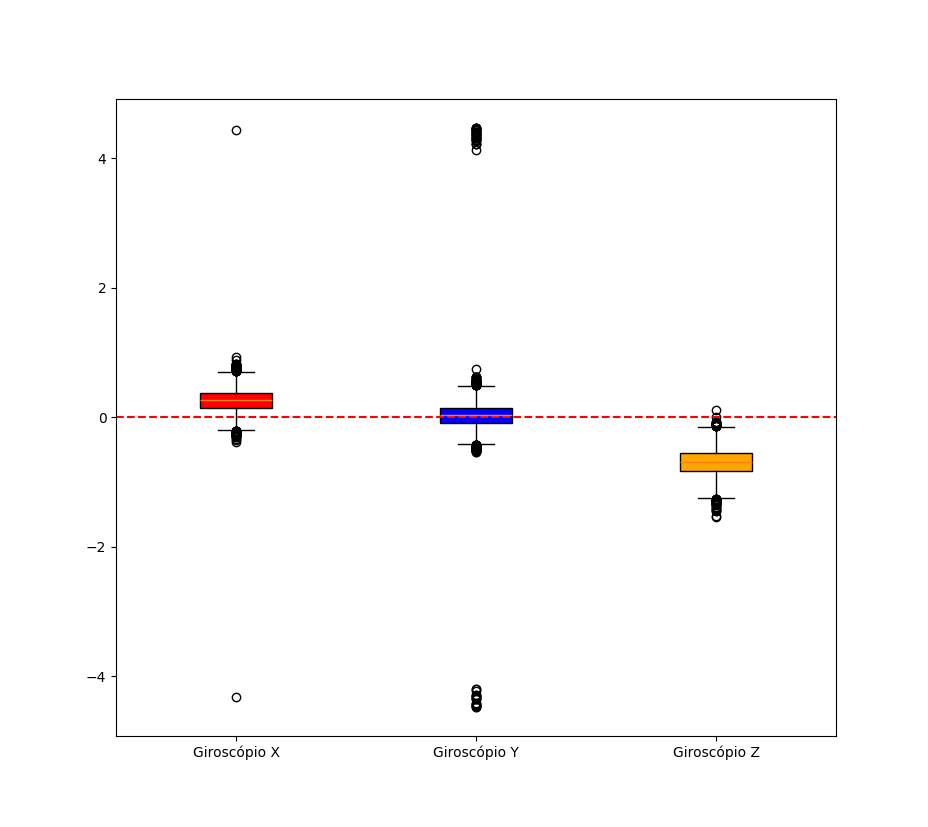
\includegraphics[width=0.8\textwidth]{dados_giroscopio_errados.png}
		\label{fig:dados_giroscopio_errado}
		\smallcaption{Fonte: Autor}
		\smallcaption{Legenda: o tracejado em vermelho representa a medida esperada em cada um dos eixos.}
	\end{figure}
	
	\begin{table}[!htb]
		\centering
		\caption{Análise estatística dos dados do giroscópio antes da calibração.}\label{tab:giroscopio_antes_calibracao}
		\begin{tabular}{|c|c|c|c|}
			\hline
			Dados & Média & Desvio Padrão ($\sigma$) & Variância ($\sigma^2$) \\ \hline
			\small Velocidade Angular X & 0.255584  & 0.176988 & 0.031325 \\ \hline
			\small Velocidade Angular Y & 0.036696  & 0.357976 & 0.128147 \\ \hline
			\small Velocidade Angular Z & -0.700549 & 0.203428 & 0.041383 \\ \hline	
		\end{tabular}
	\end{table}
	
	Assim como aconteceu com o acelerômetro, os dados mostram a necessidade da calibração do giroscópio por conta da diferença significante entre os dados coletados e as medidas esperadas. Essa grande diferença invalida a utilização do sensor, como no caso da velocidade angular em torno do eixo Z, no qual a mediana dos dados está perto de 1$^\circ/s$.
	
	A calibração do giroscópio, como descrito na Seção \ref{sec:calibracao_giroscopio}, é feita seguindo a mesma ideia da calibração do acelerômetro, sendo que no caso do primeiro são tomadas 30000 amostras contendo dados dos 3 eixos em uma única posição, diferente do segundo que necessitava de diferentes posições para uma maior precisão.
	
	A Figura \ref{fig:dados_giroscopio_certo} demonstra a correção realizada nos dados do giroscópio, visto que a mediana dos dados nos 3 eixos em 10000 amostras estão mais próximas das medidas esperadas, o que é corroborado ao observar média dos valores na Tabela \ref{tab:giroscopio_depois_calibracao}. O eixo vertical do gráfico representa a velocidade angular em $^\circ/s$.
	
	\begin{figure}[!htb]
		\centering
		\caption{10000 amostras dos dados do giroscópio depois da calibração.}
		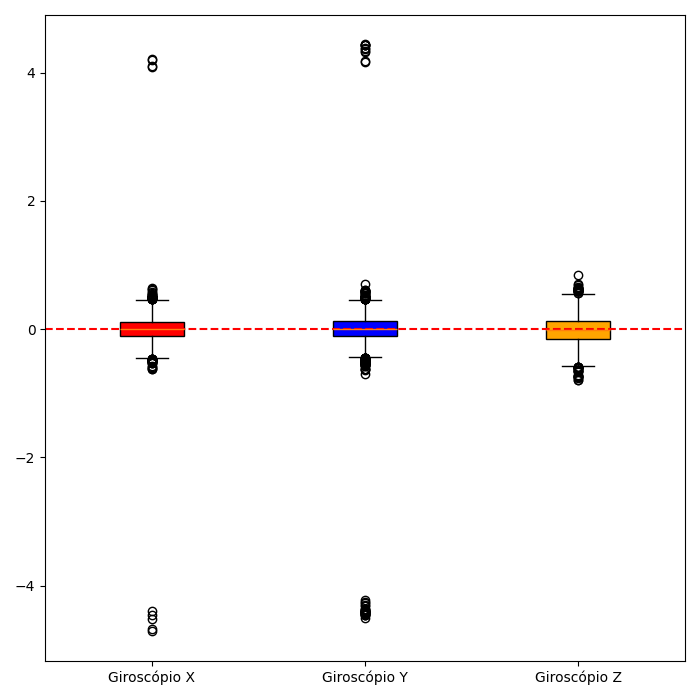
\includegraphics[width=0.8\textwidth]{dados_giroscopio_certos.png}
		\label{fig:dados_giroscopio_certo}
		\smallcaption{Fonte: Autor}
		\smallcaption{Legenda: o tracejado em vermelho representa a medida esperada em cada um dos eixos.}
	\end{figure}
	
	\begin{table}[!htb]
		\centering
		\caption{Análise estatística dos dados do giroscópio depois da calibração.}\label{tab:giroscopio_depois_calibracao}
		\begin{tabular}{|c|c|c|c|}
			\hline
			Dados & Média & Desvio Padrão ($\sigma$) & Variância ($\sigma^2$) \\ \hline
			\small Velocidade Angular X & 0.001566  & 0.210595 & 0.044350 \\ \hline
			\small Velocidade Angular Y & -0.004188  & 0.318366 & 0.101357 \\ \hline
			\small Velocidade Angular Z & -0.011643 & 0.204092 & 0.041654 \\ \hline	
		\end{tabular}
	\end{table}
	
	Apesar do êxito da calibração dos sensores, tal como aconteceu com o acelerômetro, é possível notar que existe uma certa amplitude nos dados dos giroscópio ao observar o gráfico da Figura \ref{fig:dados_giroscopio_certo} em que há muitos valores discrepantes, que são os círculos ao longo do eixo vertical.
	
	\section{TESTES}\label{sec:metodologia_testes}
	
		Nesta seção serão definidos os testes que foram realizados a fim de obter dados relevantes para análise posterior das técnicas e combinações de sensores implementadas neste trabalho.
		
		A fim de verificar qual a melhor combinação de sensores para realização da estimativa de posição utilizando \glsxtrlong{ekf} de robôs da \acrshort{ssl}, além de pontos fortes e fracos de cada combinação, foram realizados testes em dois cenários.
		
		O primeiro teste é um trajeto em forma de quadrado localizado na região central do campo, como é mostrado na Figura \ref{fig:representacao_teste_quadrado_menor}, com 70cm de lado. Como o trajeto está centralizado no campo, foi possível analisar os resultados das diferentes combinações numa região em que há sobreposição das duas câmeras utilizadas, que no caso gera um problema de o mesmo objeto ter diferentes posições por ser visto por câmeras distintas, o que é demonstrado na Figura \ref{fig:problema_overlap}.
		
		\begin{figure}[!htb]
			\centering
			\caption{Ilustração do teste de quadrado menor.}
			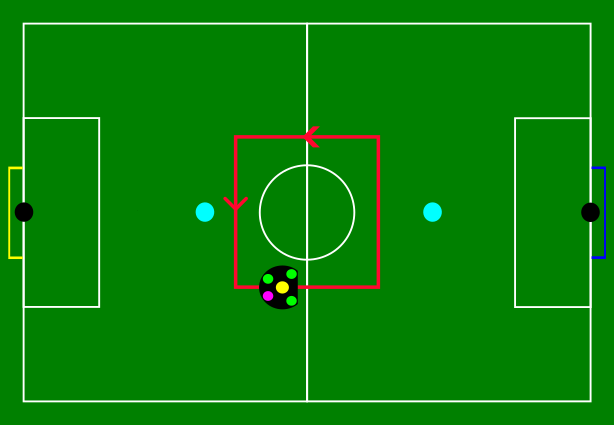
\includegraphics[width=0.80\textwidth]{representacao_teste_quadrado_menor.png}
			\label{fig:representacao_teste_quadrado_menor}
			\smallcaption{Fonte: o Autor}
		\end{figure}
	
		\begin{figure}[!htb]
			\centering
			\caption{Problema de sobreposição de câmeras.}
			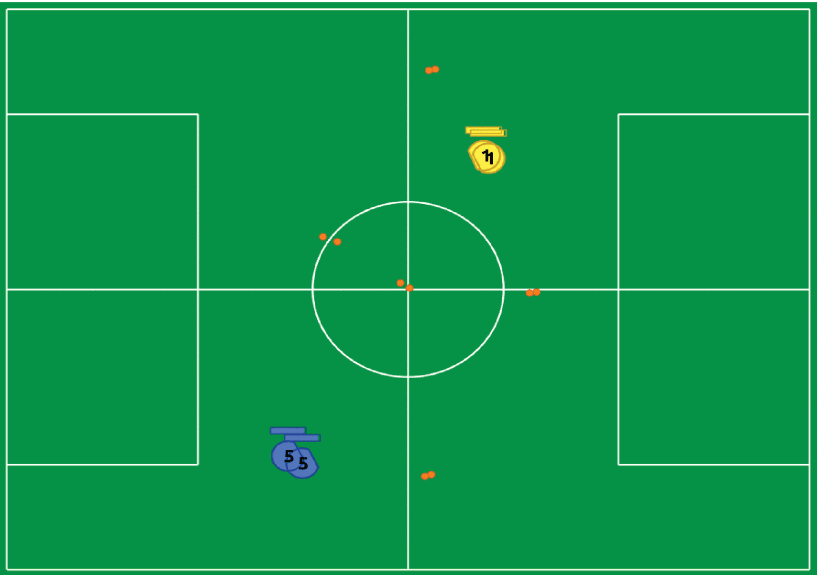
\includegraphics[width=0.85\textwidth]{problema_overlap.png}
			\label{fig:problema_overlap}
			\smallcaption{Fonte: Retirado de \textcite{9018557}}
		\end{figure}
	
		O segundo teste é um trajeto em forma de quadrado também, mas com um tamanho maior (150cm de lado) e passando por regiões do campo localizadas mais para as bordas, como é mostrado na Figura \ref{fig:representacao_teste_quadrado_maior}. Este trajeto tem o objetivo de analisar as diferentes combinações propostas de sensores em regiões localizadas nas bordas do campo, que apresentam problemas de distorção maiores causadas pela utilização de lentes olho de peixe nas câmeras. A Figura \ref{fig:problema_distorcao} mostra uma imagem que exemplifica essa distorção problemática nas bordas da imagem e, consequentemente, do campo.
			
		\begin{figure}[!htb]
			\centering
			\caption{Ilustração do teste de quadrado maior.}
			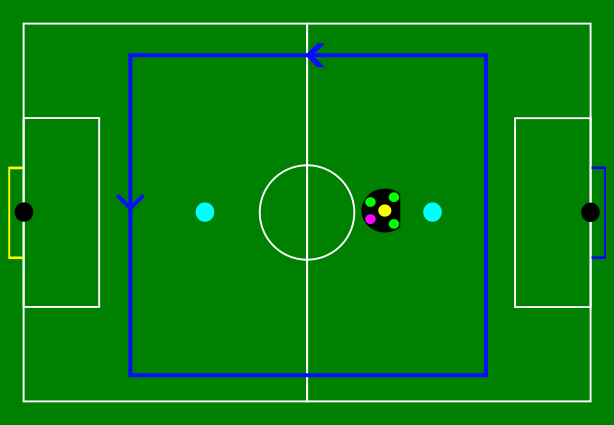
\includegraphics[width=0.80\textwidth]{representacao_teste_quadrado_maior.png}
			\label{fig:representacao_teste_quadrado_maior}
			\smallcaption{Fonte: o Autor}
		\end{figure}
	
		\begin{figure}[!htb]
			\centering
			\caption{Problema da distorção da imagem de câmeras com lente olho de peixe.}
			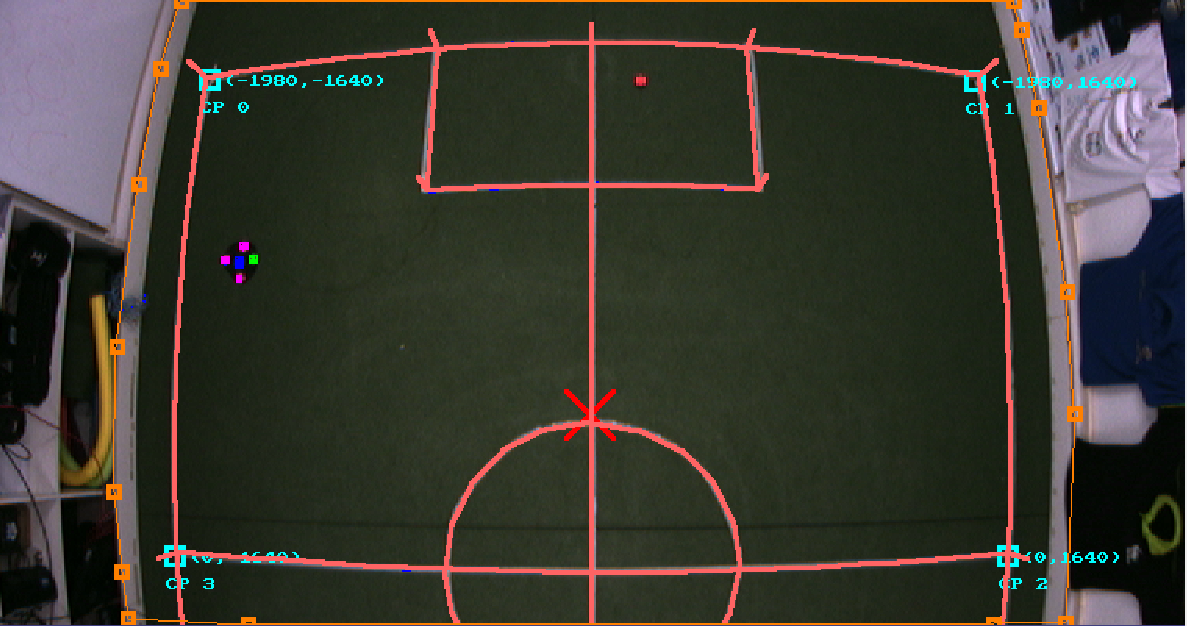
\includegraphics[width=0.80\textwidth]{problema_distorcao_2.png}
			\label{fig:problema_distorcao}
			\smallcaption{Fonte: o Autor}
		\end{figure}
	
		Os testes foram realizados com velocidade linear e angular máximas de 50$cm/s$ e 2$\pi$$rad/s$, respectivamente. É importante colocar também que, por conta do sistema de trajetórias da equipe RoboFEI o robô sempre segue o caminho proposto com a frente apontada para o vetor do trajeto, tal como demonstrado na Figuras \ref{fig:representacao_teste_quadrado_menor} e \ref{fig:representacao_teste_quadrado_maior}.
		
%		O primeiro teste a ser realizado visa extrair a resposta da posição do sistema dado uma entrada degrau a fim de analisar a qualidade das combinações de sensores propostas em relação à orientação do robô. No caso, o robô estará com sua orientação em $0^\circ$ e receberá um sinal para que ele se posicione nas mesmas coordenadas $x$ e $y$, mas com uma orientação de $180^\circ$. Este teste servirá para validar as combinações dos sensores no que tange a orientação do robô, ou seja, para isolar a análise no que diz respeito à orientação $\theta$ e não à posição ($x, y$). A ilustração do teste pode ser observada na Figura \ref{fig:metodologia_teste_1}.
%		
%		\begin{figure}[!htb]
%			\caption{Ilustração do primeiro teste.}%
%			\label{fig:metodologia_teste_1}
%			\begin{minipage}{0.45\textwidth}
%				\centering
%				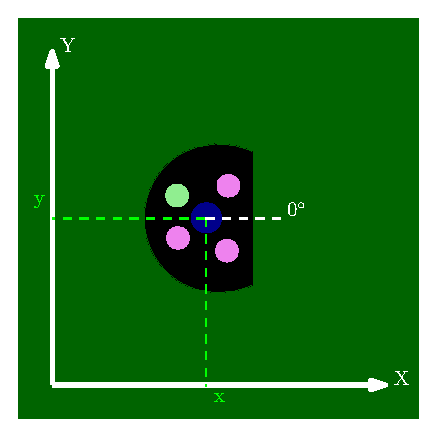
\includegraphics[width=\linewidth]{teste_1_0_graus.eps}
%				\subcaption{Posição inicial.} 
%				\label{fig:metodologia_teste_1_a}
%			\end{minipage}
%			\hfill
%			\begin{minipage}{0.45\textwidth}
%				\centering
%				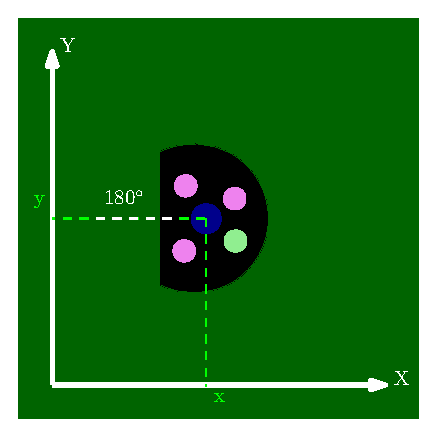
\includegraphics[width=\linewidth]{teste_1_180_graus.eps}
%				\subcaption{Posição final.} 
%				\label{fig:metodologia_teste_1_b}
%			\end{minipage}
%			\smallcaption{Fonte: o Autor}
%		\end{figure}
%		
%		O segundo cenário de teste a ser considerado é um quadrado com lado de tamanho $1.5m$ em que o robô deverá seguir seus lados com uma orientação fixa de $0^\circ$. O cenário quadrado é bastante difundido para validação de estimativa de posição \cites{rostami2018localization}{gonccalves2008real}{santini1997trajectory}. Este teste servirá para validar as combinações de sensores no que diz respeito à coordenadas $x$ e $y$ do robô, ou seja, a fim de isolar a análise no que diz respeito à posição ($x$, $y$) e não à orientação $\theta$. A ilustração do trajeto a ser realizado pode ser verificada na Figura \ref{fig:metodologia_teste_2}.
%		
%		\begin{figure}[!htb]
%			\centering
%			\caption{Ilustração do segundo teste.}
%			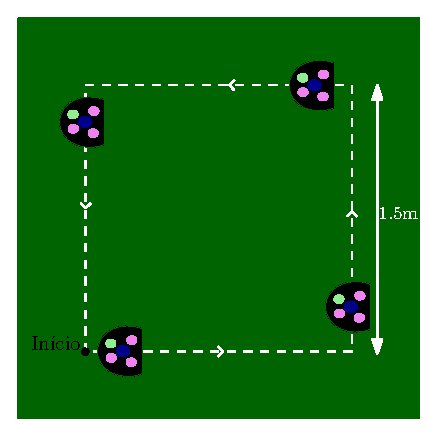
\includegraphics[width=0.6\textwidth]{teste_2.eps}
%			\label{fig:metodologia_teste_2}
%			\smallcaption{Fonte: o Autor}
%		\end{figure}
%		
%		O terceiro teste para analisar as combinações de sensores escolhidas será um círculo de raio $1m$ em que o robô deverá seguir sempre apontado para o centro do círculo. O cenário circular também é bastante difundido para validação de estimativa de posição \cites{suliman2009mobile}{marton2013two}{rigatos2010extended}{eman2020mobile}. Este teste servirá para validar as combinações tanto para a questão da orientação $\theta$ quanto para a posição ($x$, $y$) do robô. A ilustração do trajeto a ser realizado pode ser verificada na Figura \ref{fig:metodologia_teste_3}.
%		
%		\begin{figure}[!htb]
%			\centering
%			\caption{Ilustração do terceiro teste.}
%			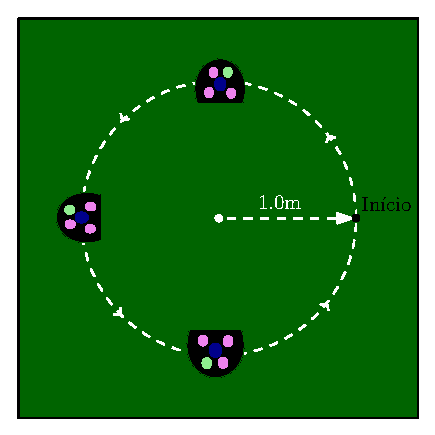
\includegraphics[width=0.6\textwidth]{teste_3.eps}
%			\label{fig:metodologia_teste_3}
%			\smallcaption{Fonte: o Autor}
%		\end{figure}
%		
%		O quarto teste será um teste que está mais inserido no ambiente do futebol de robôs. No caso, o robô terá que sair de um ponto pré-determinado dentro do campo e, a partir da localização calculada de forma embarcada, deverá alcançar a bolinha que estará em uma outra posição em campo e fazer o gol.
%		
%		Para realização desse teste, algumas mudanças devem ser feitas na estratétgia de controle de posição da equipe, visto que utiliza os dados puramente do sistema de visão para indicar qual posição cada robô deve ir e quais velocidades cada roda deve aplicar. Então, como o propósito desse projeto não é realizar o controle de posição de forma embarcada, a ideia é que ao invés de a estratégia utilizar os dados da câmera faça a utilização da posição calculada pelo filtro de Kalman e transmitida via rádio-frequência.
		
	\section{AVALIAÇÃO}\label{sec:metodologia_avaliacao}
	
		Nesta seção serão descritos os critérios de avaliação que foram utilizados para validar as diferentes combinações de sensores a fim de encontrar a melhor entre elas para realizar a estimativa de posição de um robô móvel, além de analisar os pontos positivos e negativos das combinações.
		
		A partir do feedback via rádio-frequência das posições calculadas pelo sistema de fusão de sensores embarcado, foi analisada a distância média do que é calculado de forma embarcada com o sistema de \textit{ground truth} desenvolvido. A Equação \eqref{eq:rmse_avaliacao} demonstra o cálculo do Erro Quadrático Médio (\glsxtrshort{rmse}, do inglês) da distância entre a posição calculada pelo sistema de localização utilizando fusão de sensores ($\delta_{EKF, i}$) e a posição definida pelo sistema de \textit{ground truth} ($\delta_{GTS, i}$) na amostra $i$ de um total de $n$ amostras.
		
		\begin{equation}\label{eq:rmse_avaliacao}
			RMSE = \sqrt{\frac{1}{n}\sum_{i=1}^{n}(\delta_{EKF, i} - \delta_{GTS, i})^{2}}
		\end{equation}
	
		Além da distância média durante os testes, também foi analisado o tempo de atualização das combinações. No caso, o tempo medido é o necessário para a realização dos cálculos para obtenção de uma nova estimativa de posição e velocidade do robô.
		
%		O primeiro critério de avaliação será a comparação da posição $(x, y)$ e orientação $\theta$ preditas e a real, que será medida pelo sistema de \textit{ground truth}. A segunda avaliação é o erro médio das coordenadas $(x ,y)$ e da orientação $\theta$. No caso, será analisada a diferença do que é medido pelo sistema de câmeras da \glsxtrshort{ssl} e o trajeto proposto em cada um dos testes. O terceiro critério de avaliação será o tempo gasto para completar os percursos propostos.
		
		A fim de aumentar a confiabilidade dos dados a serem extraídos, cada teste foi realizado 10 vezes. A partir deles, foram extraídos a média, desvio padrão e o valor máximo de cada uma das métricas para uma análise concisa. Em cada um dos testes foram obtidas, em média, 700 amostras no trajeto quadrado menor e 1500 amostras no trajeto quadrado maior, quantidade suficiente para análise das combinações de sensores propostas.
		
		As métricas foram escolhidas após estudos realizados nos trabalhos relacionados na área de localização de robôs móveis, sendo que a métrica do erro médio da posição estimada comparada com um \textit{ground truth} é utilizada em todos, já o tempo de atualização é importante sua análise essencialmente pela aplicação do projeto na liga de futebol de robôs \glsxtrshort{ssl} da RoboCup. A partir dessas métricas é possível avaliar a qualidade dos diferentes sensores combinados quanto a qualidade da predição de posição do robô, assim como analisar o custo computacional, sendo que o melhor sistema de localização para um robô da categoria \glsxtrshort{ssl} possui uma posição predita com o menor erro médio possível, assim como o menor tempo de atualização de estimativas.
		
	\chapter{Resultados} \label{sec:resultados}
	
		Nesta seção serão apresentados os resultados obtidos neste projeto através dos experimentos descritos na Seção \ref{sec:metodologia_testes}. Além disso, também será descrita como foi feita a aquisição do \textit{ground truth}, que serviu para comparação dos algoritmos. A fim de melhor entendimento, os resultados serão analisados graficamente ou por meio de tabelas.
		
		\section{Aquisição do ground truth} \label{sec:resultados_ground_truth}
		
			Como descrito na Seção \ref{sec:metodologia_ground_truth}, foi necessário o desenvolvimento de um sistema utilizando 2 LiDARs externos ao robô para obter o \textit{ground truth} do posicionamento do robô em campo a fim de realizar a comparação dos sistema de localização desenvolvido nesse projeto com a posição real do robô. 
			
			Embora o SSL-Vision seja utilizado como \textit{ground truth} em diversos trabalhos \cite{9018557, melo2022embedded}, nesse trabalho não é possível pelo sistema de visão global da liga ser um dos sensores considerados para comparação. Portanto, foi necessário criar um sistema de \textit{ground truth} com LiDARs externos ao robô pela necessidade de obter a posição com o robô em movimento, embora seja possível obter o \textit{ground truth} da posição manualmente com o robô parado.
			
			Nessa seção serão descritos os detalhes do sistema desenvolvido, como a técnica utilizada e a visão geral do sistema, além dos resultados alcançados pelo sistema de ground truth desenvolvido a fim de mostrar sua eficiência em comparação com a posição real do robô, medida utilizando uma trena, e com o sistema de câmeras da categoria \glsxtrshort{ssl}.
		
			\subsection{Técnica utilizada e visão geral do sistema}
				
				A Figura \ref{fig:software_architecture} mostra a arquitetura do software do sistema proposto, que é baseado num pacote do ROS2 que aplica um \textit{scan matching} para encontrar a posição relativa de ambos os lasers. Em seguida, os dados de ambos os LiDARs são combinados em uma única imagem, em que diferentes operações morfológicas são aplicadas para melhorar a qualidade dela. Na sequência a etapa de detecção acontece para reconhecimento do padrão circular na imagem e, por fim, realiza-se o cálculo da coordenada global do robô, já que o sistema em um primeiro momento calcula a posição em relação ao posicionamento dos lasers.
					
				\begin{figure}[!htb]
					\centering
					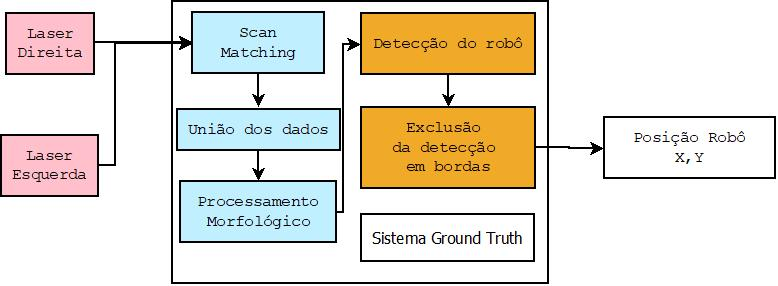
\includegraphics[width=0.80\textwidth]{software_architecture.jpeg}
					\caption{Arquitetura do software.} \label{fig:software_architecture}
				\end{figure}
			
				O primeiro estágio do sistema é a utilização do \textit{scan matching} para encontrar a transformação (translação, rotação e escala) entre as nuvens de pontos criadas a partir das leituras dos lasers que melhor encaixa os dados de ambos \cite{NIETO200739}. Essa etapa é decisiva no sistema visto que qualquer centímetro de diferença entre ambos os dados dos lasers pode levar a uma maior dificuldade para encontrar o padrão circular do robô ou pode adicionar um desvio na posição detectada.
								
				O \textit{scan matching} funciona a partir de duas nuvens de pontos, a fonte P e a alvo S. O objetivo do algoritmo é encontrar a transformação $T = (R, t)$, composta pela rotação R e translação t, que minimiza a diferença entre ambas as nuvens de pontos P e S, como descrito na Equação \eqref{eq:scan_matching}, em que $r_i$ é o ponto mais perto na nuvem de ponto alvo S.
				
				\begin{equation} \label{eq:scan_matching}
					T^* = \text{arg min} \sum_{i=1}^{n}\left\Vert (Rp_i + t) - r_i \right\Vert^2
				\end{equation}
			
				O estágio seguinte do software é a união dos dados de ambos os lasers em uma imagem, chamada de imagem de pontos do laser, aplicando a transformação encontrada na etapa de \textit{scan matching}. Para a obtenção dos dados dos sensores, foi utilizado o pacote do ROS2 desenvolvido pela SLAMTEC para ambos os lasers utilizados no sistema, já que é uma maneira mais fácil para comunicar com os sensores, inicializá-los, e receber os dados deles. O nó do ROS2 publica a mensagem do tipo \textit{laser scan} que contém as distâncias de detecção pelo sensor e seus respectivos ângulos. A partir desses dados, é possível construir a imagem de pontos do laser seguindo a Equação \eqref{eq:map_coordinates}, que demonstra como determinar as coordenadas de cada objeto detectado naquele \textit{scan}, no caso $r$ é a distância em metros e $\theta$ é o ângulo respectivo à distância detectada em radianos.
				
				\begin{equation}\label{eq:map_coordinates}
					\begin{cases}
						x = r * \cos(\theta) \\
						y = r * \sin(\theta)
					\end{cases}
				\end{equation}
			
				Depois de unir dos dados dos sensores, há uma camada para processar a imagem de pontos dos lasers antes do reconhecimento do formato circular no próximo estágio. O processamento morfológico de uma imagem é essencial para refinar a qualidade de imagens, redução de ruídos contidos nelas, e melhorar a análise estrutural delas, o que leva a uma extração de propriedades mais precisa em imagens \cite{lotufo2023morphological}. Primeiro, o algoritmo aplica uma leve dilatação dos pontos a fim de conectar pontos próximos, em seguida há uma etapa de erosão para uma melhor detecção de formatos na imagem. Finalmente, um borrão delicado é aplicado na imagem de pontos dos lasers para suavização, reduzindo o ruído na imagem e a detecção de falsos círculos, assim como ajudando na detecção do padrão.
			
				A próxima etapa do software é a detecção do robô. Esse estágio performa a detecção do padrão circular, ou semi-circular, na imagem de pontos dos lasers. O método utilizado para detecção do padrão é a transformada de Hough (\glsxtrshort{ht}). A técnica, em um primeiro momento, foi criada para detecção de linhas em imagens binárias, mas outras variações foram sugeridas para detectar diferentes formatos, como os circulares \cite{mukhopadhyay2015survey}.
				
				A \glsxtrshort{ht} para círculos utiliza da equação do círculo demonstrada na Equação \eqref{eq:circle_equation}, que o sistema calcula para cada ponto de borda na imagem pré-processada de acordo com os limites máximo e mínimo de raio definidos. Cada ponto de borda contribui com votos para possíveis círculos que ele pode fazer parte. Os votos são acumulados e o máximos locais representam as localizações dos centros e os raios dos círculos nas imagens \cite{hassanein2015survey}.
				
				\begin{equation}
					\label{eq:circle_equation}
					(x-a)^2 + (y-b)^2 = r^2
				\end{equation}
			
				Na Figura \ref{fig:robot_detection} é possível observar dois momentos da arquitetura. A Figura \ref{fig:raw_image} mostra os pontos dos lasers após os estágios de \textit{scan matching} e união dos dados, mas antes da etapa de processamento morfológico. No caso, os pontos azuis são do laser à direita do campo, enquanto os pontos verdes são do laser à esquerda. Já a Figura \ref{fig:robot_detected} mostra a etapa de detecção, em que a \glsxtrshort{ht} é aplicada na imagem de pontos dos lasers para detecção do padrão circular.
				
				\begin{figure}[!h]
					\centering
					\caption{Duas etapas da arquitetura desenvolvida.}
					\begin{subfigure}[t]{0.38\textwidth}
						\centering
						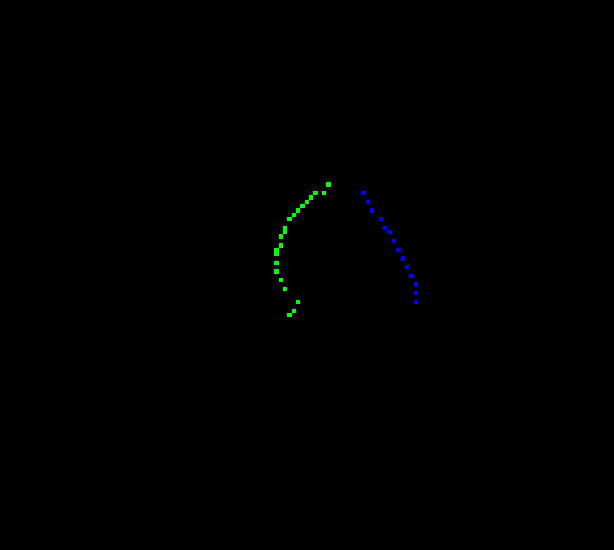
\includegraphics[width=\textwidth]{raw_lidars_image.png}
						\caption{Imagem crua dos pontos dos lasers.} \label{fig:raw_image}
					\end{subfigure}%
					\hspace{1em}
					\begin{subfigure}[t]{0.415\textwidth}
						\centering
						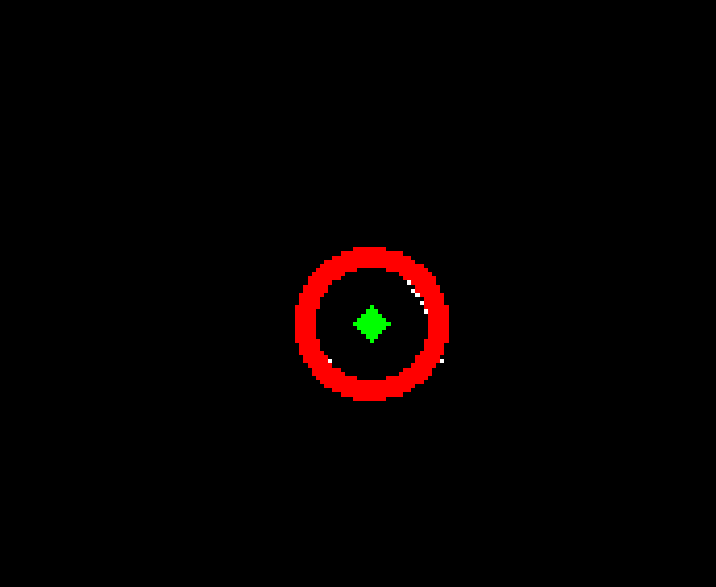
\includegraphics[width=\textwidth]{robot_detected_image.png}
						\caption{Círculo detectado pelo sistema.} \label{fig:robot_detected}
					\end{subfigure}
					\label{fig:robot_detection}
				\end{figure}
			
				A última etapa de pós-processamento é realizada para detectar e excluir falsos positivos nas bordas do campo, já que a maior parte dos pontos detectados pelo laser são os pontos da borda do campo. Basicamente, as coordenadas de fronteiras do campo são excluídas e a detecção é focada dentro do campo.
		
			\subsection{Resultados do sistema desenvolvido}
		
				Para realizar a comparação, foram decididas 17 posições arbitrárias em campo, que estão demonstradas na Figura \ref{fig:cenarios_testes_ground_truth}. Esses cenários foram escolhidos visando observar o comportamento do sistema de lasers desenvolvido em diferentes situações, no caso em posições mais centralizadas no campo (cenários centralizados, são as posições 4-6, 8-10 e 12-14), que são cenários praticamente equidistantes de ambos os lasers, e também em posições mais dispersas no campo (cenários dispersos, são as posições 1-3, 7, 11 e 15-17), onde os pontos estão consideravelmente mais perto de um laser do que outro, mas também nas beiradas do campo. Além disso, os cenários dispersos serviram para comparação com o sistema de câmeras da \glsxtrshort{ssl}, visto que por conta da distorção na utilização de lentes olho de peixe, há uma distorção maior nos cantos do campo.
				
				\begin{figure}[!htb]
					\centering
					\caption{Cenários de testes do sistema de ground truth.}
					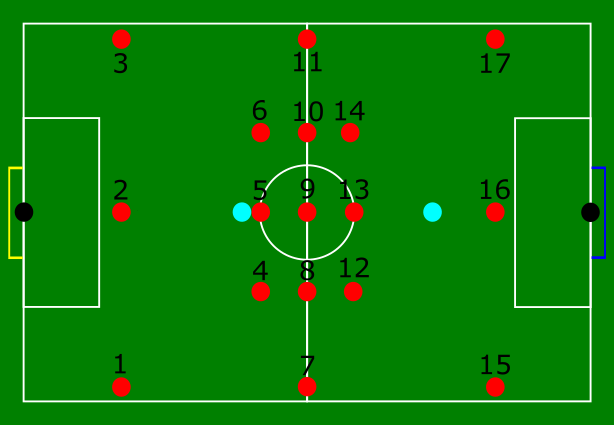
\includegraphics[width=0.6\textwidth]{cenarios_testes.png}
					\label{fig:cenarios_testes_ground_truth}
					\smallcaption{Fonte: o Autor}
					\smallcaption{Legenda: os pontos vermelhos numerados são os cenários utilizados para validar o sistema, os pontos pretos são as posições dos LiDARs em campo, enquanto os pontos azuis representam a projeção da posição das câmeras no campo.}
				\end{figure}
			
				Além dessa separação dos cenários, eles também foram separados em 3 conjuntos, que são chamados de quadrantes, que visam observar as diferenças de captura de ambos os sistemas na região de sobreposição das câmeras, localizada ao longo da região central do campo. O primeiro quadrante (posições 1-6) contém os cenários que somente a câmera da esquerda consegue capturar. O segundo quadrante (posições 7-14) é o conjunto dos cenários posicionados onde ambas câmeras conseguem capturar. Por fim, o terceiro quadrante (posições 15-17) representa os cenários em que somente a câmera à direita pode capturar. Essa separação também ajuda a entender como o sistema câmeras do \glsxtrshort{ssl} lida com a distorção separadamente. Espera-se que as coordenadas do SSL-Vision tenham um erro substancial com o distanciamento do centro das câmeras.
				
				Para poder comparar os sistemas com a posição real medida por uma trena, em cada posição foram capturadas 200 amostras do sistema de lasers, enquanto a saída do SSL-Vision também era adquirida. A média das amostras de ambos sistemas foi calculada para cada posição. Assim, é possível calcular o erro da média dos sistemas em relação ao que foi medido com a trena, assim como o desvio padrão para cada cenário a fim de analisar a estabilidade dos sistemas.
				
				As Tabelas \ref{tbl:general_results_x} e \ref{tbl:general_results_y} resumem os resultados alcançados pelo SSL-Vision, sistema de lasers e a medição real para os eixos X e Y, respectivamente, nos 17 cenários de teste. A coluna Real indica as coordenadas reais do robô com o auxílio de uma trena, enquanto as colunas Laser e Visão mostram a média e o desvio padrão das amostras medidas pelos sistemas de lasers e câmeras, respectivamente.
				
				% Please add the following required packages to your document preamble:
				% \usepackage[table,xcdraw]{xcolor}
				% Beamer presentation requires \usepackage{colortbl} instead of \usepackage[table,xcdraw]{xcolor}
				\begin{table}[!htb]
					\centering
					\caption{Resultados alcançados para o eixo X no campo de teste.}
					\label{tbl:general_results_x}
					\begin{tabular}{|c|
							>{\columncolor[HTML]{FBE2D5}}c |
							>{\columncolor[HTML]{FBE2D5}}c |
							>{\columncolor[HTML]{FBE2D5}}c |}
						\hline
						Cenário                    & Real {[}cm{]}   & Laser {[}cm{]}   & Visão {[}cm{]}   \\ \hline
						\cellcolor[HTML]{FFFFFF}1  & -91,5           & -91.797 +- 0.584 & -92.945 +- 0.026 \\ \hline
						\cellcolor[HTML]{FFFFFF}2  & -88,1           & -87.594 +- 0.437 & -89.099 +- 0.023 \\ \hline
						\cellcolor[HTML]{FFFFFF}3  & -93             & -92.510 +- 0.391 & -93.397 +- 0.049 \\ \hline
						\cellcolor[HTML]{FFFFFF}4  & -55             & -54.584 +- 0.703 & -55.389 +- 0.037 \\ \hline
						\cellcolor[HTML]{FFFFFF}5  & -51             & -50.321 +- 0.655 & -51.323 +- 0.017 \\ \hline
						\cellcolor[HTML]{FFFFFF}6  & -54,5           & -54.504 +- 0.926 & -55.363 +- 0.037 \\ \hline
						\cellcolor[HTML]{FFFFFF}7  & 0               & 1.092 +- 0.674   & 0.488 +- 0.012   \\ \hline
						\cellcolor[HTML]{FFFFFF}8  & 0               & 0.390 +- 0.624   & 0.370 +- 0.073   \\ \hline
						\cellcolor[HTML]{FFFFFF}9  & 0               & 0.552 +- 0.513   & -0.158 +- 0.061  \\ \hline
						\cellcolor[HTML]{FFFFFF}10 & 0               & 0.786 +- 0.478   & -0.505 +- 0.036  \\ \hline
						\cellcolor[HTML]{FFFFFF}11 & 0               & 0.972 +- 0.953   & 0.178 +- 0.025   \\ \hline
						\cellcolor[HTML]{FFFFFF}12 & 61,3            & 61.859 +- 0.649  & 61.588 +- 0.017  \\ \hline
						\cellcolor[HTML]{FFFFFF}13 & 52              & 51.964 +- 0.519  & 52.379 +- 0.011  \\ \hline
						\cellcolor[HTML]{FFFFFF}14 & 53              & 53.742 +- 1.036  & 52.868 +- 0.046  \\ \hline
						\cellcolor[HTML]{FFFFFF}15 & 101             & 101.653 +- 1.450 & 100.866 +- 0.015 \\ \hline
						\cellcolor[HTML]{FFFFFF}16 & 99              & 99.683 +- 0.554  & 98.785 +- 0.017  \\ \hline
						\cellcolor[HTML]{FFFFFF}17 & 97              & 97.526 +- 1.509  & 96.679 +- 0.018  \\ \hline
					\end{tabular}
				\end{table}
			
				% Please add the following required packages to your document preamble:
				% \usepackage[table,xcdraw]{xcolor}
				% Beamer presentation requires \usepackage{colortbl} instead of \usepackage[table,xcdraw]{xcolor}
				\begin{table}[!htb]
					\centering
					\caption{Resultados alcançados para o eixo Y no campo de teste.}
					\label{tbl:general_results_y}
					\begin{tabular}{|c|
							>{\columncolor[HTML]{A6C9EC}}c |
							>{\columncolor[HTML]{A6C9EC}}c |
							>{\columncolor[HTML]{A6C9EC}}c |}
						\hline
						Cenário                    & Real {[}cm{]}   & Laser {[}cm{]}    & Visão {[}cm{]}    \\ \hline
						\cellcolor[HTML]{FFFFFF}1  & -138,5          & -137.784 +- 0.726 & -139.464 +- 0.047 \\ \hline
						\cellcolor[HTML]{FFFFFF}2  & 0               & 0.844 +- 1.475    & 0.365 +- 0.018    \\ \hline
						\cellcolor[HTML]{FFFFFF}3  & 132             & 131.688 +- 0.625  & 134.255 +- 0.022  \\ \hline
						\cellcolor[HTML]{FFFFFF}4  & -85             & -84.104 +- 0.851  & -85.172 +- 0.016  \\ \hline
						\cellcolor[HTML]{FFFFFF}5  & 0               & -0.518 +- 1.424   & 0.690 +- 0.036    \\ \hline
						\cellcolor[HTML]{FFFFFF}6  & 81,5            & 80.801 +- 1.435   & 83.025 +- 0.018   \\ \hline
						\cellcolor[HTML]{FFFFFF}7  & -141            & -140.488 +- 0.742 & -139.829 +- 0.014 \\ \hline
						\cellcolor[HTML]{FFFFFF}8  & -82,5           & -82.172 +- 0.978  & -82.306 +- 0.061  \\ \hline
						\cellcolor[HTML]{FFFFFF}9  & 0               & 0.668 +- 1.052    & 0.963 +- 0.041    \\ \hline
						\cellcolor[HTML]{FFFFFF}10 & 83,5            & 84.431 +- 1.781   & 85.154 +- 0.028   \\ \hline
						\cellcolor[HTML]{FFFFFF}11 & 125,5           & 125.017 +- 0.925  & 126.895 +- 0.083  \\ \hline
						\cellcolor[HTML]{FFFFFF}12 & -92,3           & -92.848 +- 0.900  & -91.665 +- 0.015  \\ \hline
						\cellcolor[HTML]{FFFFFF}13 & 0               & -0.568 +- 0.879   & 0.810 +- 0.014    \\ \hline
						\cellcolor[HTML]{FFFFFF}14 & 85,3            & 85.046 +- 1.317   & 86.171 +- 0.053   \\ \hline
						\cellcolor[HTML]{FFFFFF}15 & -135,5          & -135.906 +- 0.813 & -135.158 +- 0.022 \\ \hline
						\cellcolor[HTML]{FFFFFF}16 & 0               & 0.048 +- 0.598    & 1.236 +- 0.016    \\ \hline
						\cellcolor[HTML]{FFFFFF}17 & 123,5           & 123.125 +- 1.015  & 124.690 +- 0.023  \\ \hline
					\end{tabular}
				\end{table}
			
				A Tabela \ref{tbl:mean_error_std} mostra o erro e desvio padrão médios em todos os cenários, mas também separadamente para os conjuntos centralizado e disperso, nos eixos X e Y. Todas as medidas estão em centímetros. É possível analisar que o erro médio para o eixo X em ambos sistemas são comparáveis, com um diferença de aproximadamente 0.1cm entre ambos. Já para o eixo Y é possível observar uma diferença considerável entre eles, perto de 0.43cm. Essa diferença pode ser explicada pela distorção ocorrida nas bordas da imagem da câmera, o que aumenta o erro nesses pontos, já que eles possuem uma distância maior das câmeras no eixo Y do que no X. 
				
				\begin{table}[!htb]
					\centering
					\caption{Erro e desvio padrão médios nos cenários.}
					\label{tbl:mean_error_std}
					\scalebox{1.00}{%
						\begin{tabular}{c|c|c|c|c|}
							\cline{2-5}
																		  	 & X - Laser & X - Visão  & Y - Laser & Y - Visão \\ \hline\hline
							\multicolumn{1}{|c|}{Erro médio}             	 & 0,5519    & 0,4461     & 0,5356    & 0,9665     \\ \hline
							\multicolumn{1}{|c|}{Erro - Centralizado}     	 & 0,4626    & 0,3785     & 0,6011    & 0,8348     \\ \hline
							\multicolumn{1}{|c|}{Erro - Disperso}       	 & 0,6523    & 0,5221     & 0,4620    & 1,1147     \\ \hline\hline
							\multicolumn{1}{|c|}{Des. Padrão médio}          & 0,7444    & 0,0305     & 1,0315    & 0,0310     \\ \hline
							\multicolumn{1}{|c|}{Des. Padrão - Centralizado} & 0,6781    & 0,0372     & 1,1796    & 0,0313     \\ \hline
							\multicolumn{1}{|c|}{Des. Padrão - Disperso}     & 0,8190    & 0,0231     & 0,8648    & 0,0306     \\ \hline
						\end{tabular}
					}
				\end{table}
			
				Os erros entre os conjuntos de cenários centralizado e disperso mostram que a câmera lida melhor com posições no centro do campo, o que é explicado pela distorção nas bordas das imagens das câmeras. Esse efeito não pode ser percebido analisando o sistema com lasers, mostrando que a detecção por eles é regular em todas as partes do campo, e prova que há vantagem na utilização de dois lasers para melhorar a detecção do padrão circular do robô em campo.
				
				Ao analisar o desvio padrão na Tabela \ref{tbl:mean_error_std}, é possível notar que o sistema de câmeras da \glsxtrshort{ssl} apresenta resultados bem mais expressivos do que o sistema com LiDARs visto que a detecção foi aproximadamente 0.3mm dispersa da média analisando todos os cenários no eixo X, e menos que 0.4mm e 0.3mm nos conjuntos centralizado e disperso, respectivamente. Já para o eixo Y os resultados foram praticamente os mesmos, comparando com o sistema do laser, este foi pior também, mas os resultados continuam aceitáveis. 
				
				Quanto a essa diferença exacerbada no desvio padrão dos dados do sistema do laser, é possível justificar isso pela resolução da imagem formada pelos dados dos lasers. Essa imagem formada é de 1000x1000 pixels, e cada pixel representa 0.533cm no campo por conta da escala utilizada para alocar os pontos na imagem. Logo, a menor diferença na detecção leva a aproximadamente 0.5cm na posição detectada do robô.
			
				Analisando os quadrantes, as Tabelas \ref{tbl:quadrant_mean_x} e \ref{tbl:quadrant_mean_y} mostram os resultados resumidos para eles nos eixos X e Y, respectivamente. Notavelmente o quadrante pertencente à câmera esquerda é pior para o eixo X ao analisar o erro médio, sendo mais que o dobro de erro comparado com os quadrantes 2 e 3. A utilização de lente olho de peixe pode explicar esse efeito já que leva a uma distorção comparável à câmera direita. Para o eixo Y em todos os quadrantes, é possível observar que o erro médio é pior quando comparado com o sistema de lasers em pelo menos 50\%. As medidas nas Tabelas \ref{tbl:quadrant_mean_x} e \ref{tbl:quadrant_mean_y} também estão em centímetros.
				
				\begin{table}[!htb]
					\centering
					\caption{Resultados dos quadrantes para o eixo X.}
					\label{tbl:quadrant_mean_x}
					\scalebox{0.97}{%
						\begin{tabular}{c|c|c|c|c|}
							\cline{2-5}
							& \multicolumn{1}{l|}{\textbf{Erro X - Laser}} & \multicolumn{1}{l|}{\textbf{Erro X - Vis.}} & \textbf{Des. Padrão X - Laser} & \textbf{Des. Padrão X - Vis.} \\ \hline
							\multicolumn{1}{|l|}{\textbf{Quad. 1}} & 0,3986                                        & 0,7360                                         & 0,6224                       & 0,0315                        \\ \hline
							\multicolumn{1}{|l|}{\textbf{Quad. 2}} & 0,6411                                        & 0,3122                                         & 0,6807                       & 0,0351                        \\ \hline
							\multicolumn{1}{|l|}{\textbf{Quad. 3}} & 0,6206                                        & 0,2233                                         & 1,1710                       & 0,01667                       \\ \hline
						\end{tabular}
					}
				\end{table}
				
				\begin{table}[!htb]
					\centering
					\caption{Resultados dos quadrantes para o eixo Y.}
					\label{tbl:quadrant_mean_y}
					\scalebox{0.97}{%
						\begin{tabular}{c|c|c|c|c|}
							\cline{2-5}
							& \textbf{Erro Y - Laser} & \textbf{Erro Y - Vis.} & \textbf{Des. Padrão Y - Laser} & \textbf{Des. Padrão Y - Vis.} \\ \hline
							\multicolumn{1}{|c|}{\textbf{Quad. 1}} & 0,6641                   & 0,9951                  & 1,0893                       & 0,0261                      \\ \hline
							\multicolumn{1}{|c|}{\textbf{Quad. 2}} & 0,5844                   & 1,0754                  & 1,0956                       & 0,0454                      \\ \hline
							\multicolumn{1}{|c|}{\textbf{Quad. 3}} & 0,3665                   & 0,8473                  & 0,9203                       & 0,0238                      \\ \hline
						\end{tabular}
					}
				\end{table}
			
				Ao analisar o desvio padrão, não é notável qualquer influência do posicionamento das câmeras em ambos os eixos. Além disso, o SSL-Vision continua melhor que o sistema de lasers em todos os quadrantes para X e Y. Quando analisado para ambos os eixos, não é possível analisar diferenças significativas entre os quadrantes para o sistema de lasers, mostrando que a detecção realizada por ele é regular, e os erros acumulados em longas distâncias para um laser são compensados pelas leituras do outro laser.
				
%		\section{Parametrização das covariâncias}
%		
%			A parametrização das variâncias dos sensores é parte importante do projeto do \glsxtrlong{ekf}, principalmente para a estimativa das matrizes de covariância dos ruídos de processo e medições, respectivamente, $Q_{k}$ e $R_{k}$, visto que elas impõe quanta confiança se coloca nos valores do estado estimado.
%			
%			A partir disso, para definir o desvio padrão das posições globais X e Y e da orientação a partir dos sensores foram capturadas 1000 amostras dessas variáveis com o robô parado, já para definir o desvio padrão das velocidades locais X e Y, foram capturadas 1000 amostras dessas variáveis com o robô andando numa velocidade constante de 0.2$m/s$. Então, a partir dessas amostras é calculado o desvio padrão de cada variável dita.
		
		\section{Implementação dos cenários}
		
			Nesta Seção serão abordadas as implementações dos cenários de fusão de sensores propostos na Seção \ref{sec:metodologia_comb_sensores}. Os estados definidos para os cenários desse trabalho seguem o que é descrito na Equação \eqref{eq:estados_do_sistema}, em que $\textbf{X}$ é o vetor de estados do sistema no instante de tempo $k$. No caso, os estados do sistema são as posições globais $x$ e $y$ e orientação $\theta$ do robô em campo, e pelas velocidades locais do robô $v_{x}$ e $v_{y}$. 
			
			\begin{equation}\label{eq:estados_do_sistema}
				\text{\textbf{X}}_k =
				\begin{bmatrix}
					x_{k} \\
					y_{k} \\
					\theta_{k} \\
					v_{x,k} \\
					v_{y,k}
				\end{bmatrix}
			\end{equation}
		
			\subsection{Cenário 1 - Modelo + Visão} \label{sec:implementacao_cenario_1}
			
				O primeiro cenário utiliza do modelo cinemático de um robô omnidirecional na fase de predição e os dados do sistema global de visão na fase de correção.
				
				As entradas do sistema para esse cenário são as velocidades locais do robô nos eixos X e Y e a angular ($v_{x,teór}$, $v_{y,teór}$ e $\omega_{teór}$, respectivamente) calculadas pelo sistema de planejamento de trajetória da equipe, representada pelo vetor $\text{\textbf{u}}_k$, conforme a Equação \eqref{eq:entrada_predicao_modelo}. O índice $teór$ representa que as variáveis são adquiridas a partir do modelo cinemático do robô.
				
				\begin{equation}\label{eq:entrada_predicao_modelo}
					\text{\textbf{u}}_k =
					\begin{bmatrix}
						v_{x,teór} \\
						v_{y,teór} \\
						\omega_{teór}
					\end{bmatrix}
				\end{equation}
			
				A Equação \eqref{eq:predicao_cenario_1} mostra a atualização dos estados na fase de predição do sistema de localização nesse cenário. Os índices $k$ e $k-1$ representam o instante de tempo daquela variável, no caso os instantes atual e passado, respectivamente, tanto para esse quanto para os próximos cenários. Já o índice $G$ representa as variáveis descritas nos eixos globais do campo, como no caso das velocidades nos eixos X e Y do campo $V_{x,G}$ e $V_{y,G}$, respectivamente. A variável $\Delta_t$ representa a variação de tempo, em segundos.
				
				\begin{equation}\label{eq:predicao_cenario_1}
					\begin{cases}
						x_{k} = x_{k-1} + V_{x,G} \Delta_t \\
						y_{k} = y_{k-1} + V_{y,G} \Delta_t  \\
						\theta_{k} = \theta_{k-1} + \omega_{teór,k} \Delta_t \\
						v_{x,k} = v_{x,teór,k}\\
						v_{y,k} = v_{y,teór,k}
					\end{cases}
				\end{equation}
			
			Para o cálculo das posições globais do robô é necessário que as velocidades estejam descritas em relação ao eixo do campo, no caso descritas como $V_{x,G}$ e $V_{y,G}$, e são calculadas conforme a Equação \eqref{eq:calculo_velocidades_globais}. É importante notar a transformação feita subtraindo $\frac{\pi}{2}$ do ângulo calculado do robô para alinhar os eixos locais do robô com os eixos globais do campo, conforme a Figura \ref{fig:representacao_eixos_robo_campo}, em que o eixo em azul representa a convenção adotada pelo sistema de visão da \glsxtrshort{ssl}, enquanto o eixo em vermelho representa a convenção adotada pela equipe para o robô. Esse conceito de transformação será utilizado tanto nesse quantos nos próximos cenários.
			
				\begin{equation}\label{eq:calculo_velocidades_globais}
					\begin{cases}
						V_{x,G} = \cos(\theta_{k-1} - \frac{\pi}{2}) \times v_{x,teór,k-1} - \sin(\theta_{k-1} - \frac{\pi}{2}) \times v_{y,teór,k-1} \\
						V_{y,G} = \sin(\theta_{k-1} - \frac{\pi}{2}) \times v_{x,teór,k-1} + \cos(\theta_{k-1} - \frac{\pi}{2}) \times v_{y,teór,k-1}
					\end{cases}
				\end{equation}
			
			\begin{figure}[!htb]
				\centering
				\caption{Diferença entre os eixos do campo e do robô.}
				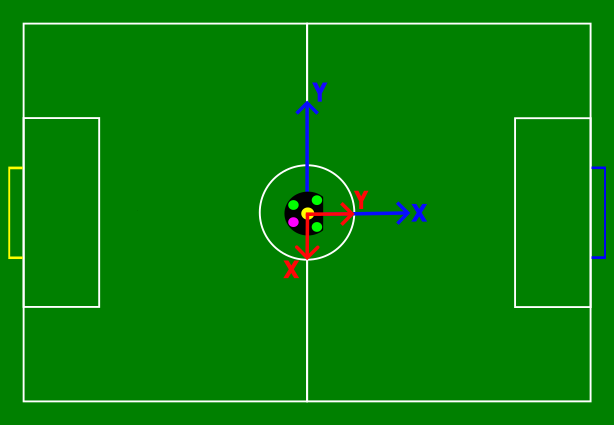
\includegraphics[width=1.0\textwidth]{representacao_eixos_robo_campo.png}
				\label{fig:representacao_eixos_robo_campo}
				\smallcaption{Fonte: o Autor}
			\end{figure}
		
			 A partir disso, a matriz jacobiana $G_k$ dos estados previstos em relação ao estado anterior segue a Equação \eqref{eq:matriz_G_cenario_1}.
		
			\begin{equation}\label{eq:matriz_G_cenario_1}
			 	G_{k} = \begin{bmatrix}
			 		1 & 0 & (\cos(\theta)v_x\Delta_t - \sin(\theta)v_y\Delta_t) & \sin(\theta)\Delta_t & \cos(\theta)\Delta_t \\
			 		0 & 1 & (\sin(\theta)v_x\Delta_t - \cos(\theta)v_y\Delta_t) & -\cos(\theta)\Delta_t & \sin(\theta)\Delta_t \\
			 		0 & 0 & 1 & 0 & 0 \\
			 		0 & 0 & 0 & 0 & 0 \\
			 		0 & 0 & 0 & 0 & 0 \\
			 	\end{bmatrix}
			 \end{equation}
		 
		 	Já a matriz de covariância dos ruídos do processo $Q_{k}$ é definida na Equação \eqref{eq:matriz_cov_processo_cenario_1}.
		 	
		 	\begin{equation}\label{eq:matriz_cov_processo_cenario_1}
		 		Q_{k} = \begin{bmatrix}
		 			2.34\cdot10^{-4} & 0 & 0 & 0 & 0 \\
		 			0 & 2.34\cdot10^{-4} & 0 & 0 & 0 \\
		 			0 & 0 & 2.23\cdot10^{-5} & 0 & 0 \\
		 			0 & 0 & 0 & 1\cdot10^{-4} & 0 \\
		 			0 & 0 & 0 & 0 & 1\cdot10^{-4} \\
		 		\end{bmatrix}
		 	\end{equation}
		 
			 Quanto à fase de correção, nesse cenário são utilizados os dados de posição do sistema global de câmeras da \glsxtrshort{ssl}. Conforme a Equação \eqref{eq:estados_correcao_cenario_1}, o sistema de visão providencia observações diretas tanto das posições globais $x$ e $y$ dos robôs, quanto da orientação $\theta$, com um certo ruído. O vetor de medições é apresentado pelo vetor $\textbf{z}_k$.
			 
	 		\begin{equation}\label{eq:estados_correcao_cenario_1}
			 	\textbf{z}_k  = 
			 	\begin{bmatrix}
			 		x_k \\
			 		y_k \\
			 		\theta_k
			 	\end{bmatrix}
			\end{equation}
		 
		 	A partir disso, a matriz de transformação do estado real no estado observado $C_k$ é definida na Equação \eqref{eq:matriz_C_cenario_1}. Já a matriz de covariância $R_{k}$ das medições do sistema global de câmeras é definida na Equação \eqref{eq:matriz_cov_medicoes_cenario_1}.
			 
			\begin{equation}\label{eq:matriz_C_cenario_1}
			 	C_{k} = \begin{bmatrix}
			 		1 & 0 & 0 \\
			 		0 & 1 & 0 \\
			 		0 & 0 & 1 \\
			 	\end{bmatrix}
		 	\end{equation}
	 	
	 		\begin{equation} \label{eq:matriz_cov_medicoes_cenario_1}
	 			R_{k} = \begin{bmatrix}
	 				1.35\cdot10^{-6} & 0 & 0 \\
	 				0 & 1.35\cdot10^{-6} & 0 \\
	 				0 & 0 & 9.74\cdot10^{-5} \\
	 			\end{bmatrix}
	 		\end{equation}
		
		\subsection{Cenário 2 - Modelo + Encoders} \label{sec:implementacao_cenario_2}
		
			O segundo cenário também utiliza do modelo cinemático de um robô omnidirecional na fase de predição do \glsxtrshort{ekf}, mas utiliza os dados dos encoders acoplados às rodas na fase de correção.
			
			A atualização dos estados na fase de predição do sistema de localização segue a Equação \eqref{eq:predicao_cenario_1} definida na Seção \ref{sec:implementacao_cenario_1}, sendo as entradas definidas na Equação \eqref{eq:entrada_predicao_modelo}. A matriz jacobiana $G_k$ é definida na Equação \eqref{eq:matriz_G_cenario_1}, enquanto a matriz dos ruídos do processo $Q_k$ segue a Equação \eqref{eq:matriz_cov_processo_cenario_1}.
			
			Para a fase de correção, são utilizados os dados dos encoders acoplados às rodas a fim de obter uma estimativa melhor das velocidades locais X e Y do robô e, assim das posições globais e da orientação, como demonstrado pelo vetor de medições $\textbf{z}_k$ na Equação \eqref{eq:estados_correcao_cenario_2}. O índice $enc$ nas variáveis demonstra que os estados do sistema são calculados a partir dos dados dos encoders, no caso as posições globais $x_{enc}$ e $y_{enc}$, orientação $\theta_{enc}$ e velocidades locais $v_{x,enc}$ e $v_{y,enc}$
			
	 		\begin{equation}\label{eq:estados_correcao_cenario_2}
				\textbf{z}_k  = 
				\begin{bmatrix}
					x_{enc,k} \\
					y_{enc,k} \\
					\theta_{enc,k} \\
					v_{x,enc,k} \\
					v_{y,enc,k}
				\end{bmatrix}
			\end{equation}
		
			A Equação \eqref{eq:correcao_cenario_2} demonstra como os estados para a fase de correção são atualizados com as leituras dos encoders, sendo que $\Delta_t$ representa o intervalo de tempo entre uma etapa de correção e outra. Já a variável $\omega_{enc}$ representa a velocidade angular provida pelos encoders.
			
			\begin{equation}\label{eq:correcao_cenario_2}
				\begin{cases}
					x_{enc,k} = x_{enc,k-1} + V_{x,enc,G} \Delta_t \\
					y_{enc,k} = y_{enc,k-1} + V_{y,enc,G} \Delta_t  \\
					\theta_{enc,k} = \theta_{enc,k-1} + \omega_{enc,k} \Delta_t \\
					v_{x,enc,k} = v_{x,enc,k}\\
					v_{y,enc,k} = v_{y,enc,k}
				\end{cases}
			\end{equation}
			
			O cálculo das velocidades globais para determinar as posições globais segue a ideia da Equação \eqref{eq:calculo_velocidades_globais}. Porém, na Equação \eqref{eq:calculo_velocidades_globais_encoder}, para o cálculo de $V_{x,enc,G}$ e $V_{y,enc,G}$, as velocidades locais utilizadas são providas a partir dos encoders.
			
				\begin{equation}\label{eq:calculo_velocidades_globais_encoder}
					\begin{cases}
						V_{x,enc,G} = \cos(\theta_{enc,k-1} - \frac{\pi}{2}) \times v_{x,enc,k} - \sin(\theta_{enc,k} - \frac{\pi}{2}) \times v_{y,enc,k} \\
						V_{y,enc,G} = \sin(\theta_{enc,k-1} - \frac{\pi}{2}) \times v_{x,enc,k} + \cos(\theta_{enc,k} - \frac{\pi}{2}) \times v_{y,enc,k}
					\end{cases}
				\end{equation}
			
			A partir disso, a matriz $C_{k}$ de transformação do estado real no estado observado segue a Equação \eqref{eq:matriz_C_cenario_2}.
			
			\begin{equation}\label{eq:matriz_C_cenario_2}
				C_{k} = \begin{bmatrix}
					1 & 0 & 0 & 0 & 0 \\
					0 & 1 & 0 & 0 & 0 \\
					0 & 0 & 1 & 0 & 0 \\
					0 & 0 & 0 & 1 & 0 \\
					0 & 0 & 0 & 0 & 1
				\end{bmatrix}
			\end{equation}
			
			A matriz de covariância dos ruídos das medições $R_{k}$ desse cenário é definida na Equação \eqref{eq:matriz_cov_medicoes_cenario_2}.
			
			\begin{equation}\label{eq:matriz_cov_medicoes_cenario_2}
				R_{k} = \begin{bmatrix}
					2.50\cdot10^{-6} & 0 & 0 & 0 & 0 \\
					0 & 2.50\cdot10^{-6} & 0 & 0 & 0 \\
					0 & 0 & 5\cdot10^{-6} & 0 & 0 \\
					0 & 0 & 0 & 2.50\cdot10^{-6} & 0 \\
					0 & 0 & 0 & 0 & 2.50\cdot10^{-6}
				\end{bmatrix}
			\end{equation}
		
		\subsection{Cenário 3 - Modelo + \glsxtrshort{imu}} \label{sec:implementacao_cenario_3}
		
			O terceiro cenário também utiliza do modelo cinemático de um robô omnidirecional na fase de predição do \glsxtrshort{ekf}, enquanto na fase de correção são utilizados os dados da \glsxtrshort{imu} presente na placa principal do robô.
			
			Para a fase de predição, o conceito segue o que foi descrito nas Seções \ref{sec:implementacao_cenario_1} e \ref{sec:implementacao_cenario_2}. Já para a fase de correção, são utilizadas as leituras da \glsxtrshort{imu} (giroscópio + acelerômetro) para obter uma estimativa dos estados do sistema. As variáveis com índice $imu$ são as calculadas a partir dos dados da \acrshort{imu}, no caso as posições globais $x_{imu}$ e $y_{imu}$, orientação $\theta_{imu}$ e velocidades locais $v_{x,imu}$ e $v_{y,imu}$ do robô, conforme o que é descrito na Equação \eqref{eq:estados_correcao_cenario_3} no vetor $\textbf{z}_k$.
			
	 		\begin{equation}\label{eq:estados_correcao_cenario_3}
				\textbf{z}_k  = 
				\begin{bmatrix}
					x_{imu,k} \\
					y_{imu,k} \\
					\theta_{imu,k} \\
					v_{x,imu,k} \\
					v_{y,imu,k}
				\end{bmatrix}
			\end{equation}
		
			A Equação \eqref{eq:correcao_cenario_3} demonstra como os estados para a fase de correção são atualizados com as leituras do giroscópio e acelerômetro. As variáveis $V_{x,imu,G}$ e $V_{y,imu,G}$ são as velocidades globais calculadas a partir dos dados da \acrshort{imu}, enquanto as variáveis $A_{x,imu,G}$ e $A_{y,imu,G}$ indicam as acelerações calculadas nos eixos globais do campo. $\Delta_t$ representa o intervalo de tempo entre os instantes $k$ e $k-1$.
			
			\begin{equation}\label{eq:correcao_cenario_3}
				\begin{cases}
					x_{imu,k} = x_{imu, k-1} + V_{x,imu,G} \Delta_t + \frac{1}{2}A_{x,imu,G} \Delta_t^2 \\
					y_{imu,k} = y_{imu, k-1} + V_{y,imu,G} \Delta_t + \frac{1}{2}A_{y,imu,G} \Delta_t^2 \\
					\theta_{imu,k} = \theta_{imu, k-1} + \omega_{imu,k} \Delta_t \\
					v_{x,imu,k} = v_{x,imu,k-1} + a_{x,k} \Delta_t\\
					v_{y,imu,k} = v_{y,imu,k-1} + a_{y,k} \Delta_t
				\end{cases}
			\end{equation}
		
			No caso da \acrshort{imu}, tanto as velocidades globais quanto as leituras de aceleração precisam ser transformadas para os eixos globais do campo. Sendo assim, as Equações \eqref{eq:calculo_velocidades_globais_imu} e \eqref{eq:calculo_aceleracoes_globais_imu} demonstram a transformação feita para ambos os componentes. As variáveis $a_{x}$ e $a_{y}$ representam as acelerações nos eixos locais X e Y do robô.
		
			\begin{equation}\label{eq:calculo_velocidades_globais_imu}
				\begin{cases}
					V_{x,imu,G} = \cos(\theta_{imu,k-1} - \frac{\pi}{2}) \times v_{x,imu,k-1} - \sin(\theta_{imu,k-1} - \frac{\pi}{2}) \times v_{y,imu,k-1} \\
					V_{y,imu,G} = \sin(\theta_{imu,k-1} - \frac{\pi}{2}) \times v_{x,imu,k-1} + \cos(\theta_{imu,k-1} - \frac{\pi}{2}) \times v_{y,imu,k-1}
				\end{cases}
			\end{equation}
		
			\begin{equation}\label{eq:calculo_aceleracoes_globais_imu}
				\begin{cases}
					A_{x,imu,G} = \cos(\theta_{imu,k-1} - \frac{\pi}{2}) \times a_{x,k} - \sin(\theta_{imu,k-1} - \frac{\pi}{2}) \times a_{y,k} \\
					A_{y,imu,G} = \sin(\theta_{imu,k-1} - \frac{\pi}{2}) \times a_{x,k} + \cos(\theta_{imu,k-1} - \frac{\pi}{2}) \times a_{y,k}
				\end{cases}
			\end{equation}
		
			A partir disso, a matriz $C_k$ de transformação do estado real no estado observado segue a Equação \eqref{eq:matriz_C_cenario_3}, já que a correção a partir dos dados da IMU provê observações diretas sobre todos os estados do sistema.
			
			\begin{equation}\label{eq:matriz_C_cenario_3}
				C_{k} = \begin{bmatrix}
					1 & 0 & 0 & 0 & 0 \\
					0 & 1 & 0 & 0 & 0 \\
					0 & 0 & 1 & 0 & 0 \\
					0 & 0 & 0 & 1 & 0 \\
					0 & 0 & 0 & 0 & 1
				\end{bmatrix}
			\end{equation}
		
			A matriz de covariância dos ruídos das medições $R_{k}$ desse cenário é definida na Equação \eqref{eq:matriz_cov_medicoes_cenario_3}.
			
			\begin{equation}\label{eq:matriz_cov_medicoes_cenario_3}
				R_{k} = \begin{bmatrix}
					7.04\cdot10^{-5} & 0 & 0 & 0 & 0 \\
					0 & 7.04\cdot10^{-5} & 0 & 0 & 0 \\
					0 & 0 & 4.04\cdot10^{-4} & 0 & 0 \\
					0 & 0 & 0 & 2.5\cdot10^{-3} & 0 \\
					0 & 0 & 0 & 0 & 2.5\cdot10^{-3}
				\end{bmatrix}
			\end{equation}
		
			É importante pontuar que ao utilizar a \glsxtrshort{imu} para a fase de correção, tanto nesse quanto nos outros cenários, é feita a integração da aceleração provida pelo acelerômetro a fim de estimar a velocidade e posição do robô. Entretanto, ao fazer essa integração, por conta do alto ruído presente nos dados do sensor, acaba-se acumulando um grande erro em um curto espaço de tempo. Esse efeito pode ser observado na Figura \ref{fig:comparacao_velocidade_accel_encoder}, que compara a velocidade local no eixo Y obtida a partir tanto da \glsxtrshort{imu} (vermelho) quanto dos encoders (azul), enquanto a Figura \ref{fig:comparacao_acelerometro_x_y} mostra as leituras do acelerômetro durante o trajeto. É notável que durante o começo do movimento a integração da aceleração tem resultados parecidos com a velocidade dos encoders, mas depois de um tempo os erros da integração começam a crescer desenfreadamente.
			
%			\begin{figure}[!htb]
%				\centering
%				\caption{Diferença das velocidades calculadas pelo acelerômetro e pelos encoders.}
%				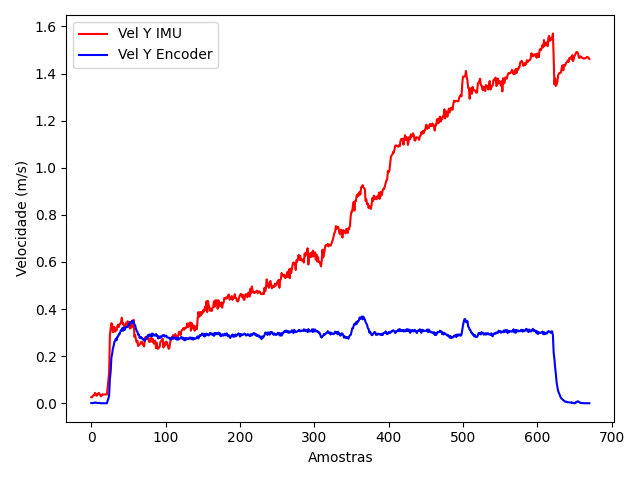
\includegraphics[width=0.7\textwidth]{comparacao_velocidade_accel_encoder.png}
%				\label{fig:comparacao_velocidade_accel_encoder}
%				\smallcaption{Fonte: o Autor}
%			\end{figure}

			\begin{figure}
				\centering
				\begin{minipage}[t]{0.47\textwidth}
					\centering
					\caption{Diferença das velocidades calculadas pelo acelerômetro e pelos encoders.}
					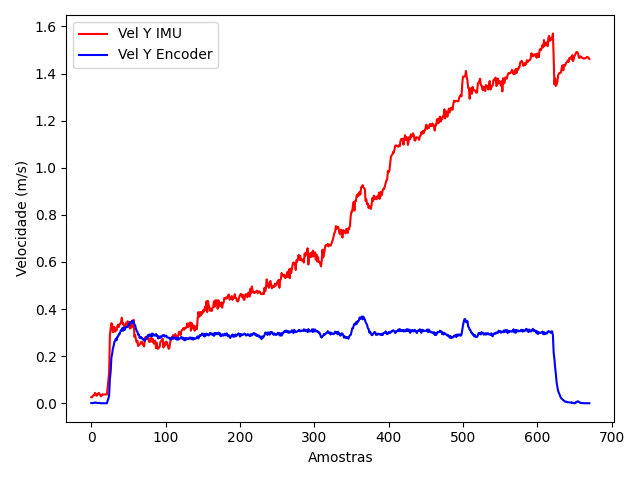
\includegraphics[width=\textwidth]{comparacao_velocidade_accel_encoder.png}
					\label{fig:comparacao_velocidade_accel_encoder}
					\smallcaption{Fonte: o Autor}
				\end{minipage}
				\hspace{1em}
				\begin{minipage}[t]{0.47\textwidth}
					\centering
					\caption{Acelerações obtidas durante o teste.}
					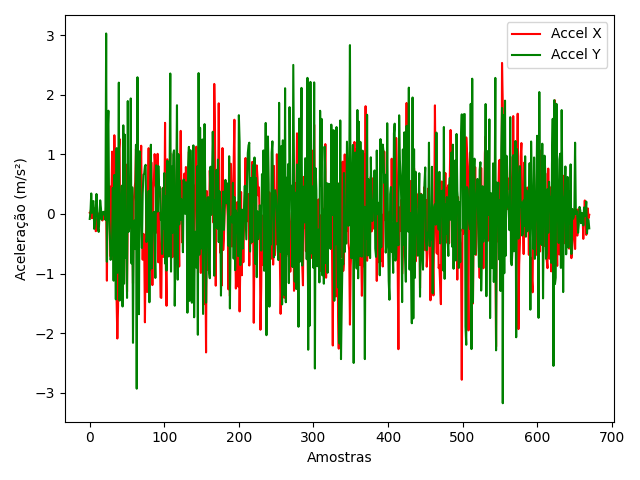
\includegraphics[width=\textwidth]{dados_acelerometro_x_y.png}
					\label{fig:comparacao_acelerometro_x_y}
					\smallcaption{Fonte: o Autor}
				\end{minipage}
			\end{figure}
			
			Para impedir esse acúmulo de erro desenfreado a longo prazo, decidiu-se que as velocidades locais $v_{x,imu}$ e $v_{y,imu}$ calculadas a partir da \acrshort{imu}, a cada 5 ciclos de correção performados pelo \glsxtrshort{ekf}, são definidas como as velocidades locais $v_{x}$ e $v_{y}$ estimadas pelo filtro, seguindo a Equação \eqref{eq:velocidade_imu_estimada_ekf}.
			
			\begin{equation}\label{eq:velocidade_imu_estimada_ekf}
				\begin{cases}
					v_{x,imu,k} = v_{x,k} \\
					v_{y,imu,k} = v_{y,k}
				\end{cases}
			\end{equation}
		
		\subsection{Cenário 4 - \glsxtrshort{imu} + Visão} \label{sec:implementacao_cenario_4}
		
			Nesse cenário 4, os dados da \glsxtrshort{imu} são utilizados na fase de predição do \glsxtrshort{ekf}, enquanto na fase de correção são utilizados os dados do sistema global de câmeras da categoria \glsxtrshort{ssl}.
			
			Para a fase de predição do \glsxtrshort{ekf}, os dados do acelerômetro são utilizados para predizer tanto as posições globais $x$ e $y$ quanto as velocidades locais $v_{x}$ e $v_{y}$ nos X e Y do robô, enquanto os dados do giroscópio são utilizados para predizer a orientação $\theta$ do robô em campo. A Equação \eqref{eq:predicao_cenario_4} mostra como é feita a atualização de cada um dos estados com os dados da \acrshort{imu}, sabendo do intervalo de tempo $\Delta_t$ entre um instante e outro. O vetor de entrada do sistema $\textbf{u}_k$ é composto pelas acelerações locais $a_{x}$ e $a_{y}$ nos eixos X e Y do robô, assim como a velocidade angular $\omega$ do robô, como está descrito na Equação \eqref{eq:entrada_predicao_imu}.
			
			\begin{equation}\label{eq:entrada_predicao_imu}
				\text{\textbf{u}}_k =
				\begin{bmatrix}
					a_{x} \\
					a_{y} \\
					\omega
				\end{bmatrix}
			\end{equation}
			
			\begin{equation}\label{eq:predicao_cenario_4}
				\begin{cases}
					x_{k} = x_{k-1} + V_{x,G} \Delta_t + \frac{1}{2}A_{x,imu,G} \Delta_t^2 \\
					y_{k} = y_{k-1} + V_{y,G} \Delta_t + \frac{1}{2}A_{y,imu,G} \Delta_t^2 \\
					\theta_{k} = \theta_{k-1} + \omega_{k} \Delta_t \\
					v_{x,k} = v_{x,k-1} + a_{x,k} \Delta_t\\
					v_{y,k} = v_{y,k-1} + a_{y,k} \Delta_t
				\end{cases}
			\end{equation}

			O cálculo das velocidades globais desse cenário segue o que é descrito na Equação \eqref{eq:calculo_velocidades_globais}, enquanto a transformação das acelerações locais para globais é demonstrada na Equação \eqref{eq:calculo_aceleracoes_globais}.
			
			\begin{equation}\label{eq:calculo_aceleracoes_globais}
				\begin{cases}
					A_{x,imu,G} = \cos(\theta_{k-1} - \frac{\pi}{2}) \times a_{x,k} - \sin(\theta_{k-1} - \frac{\pi}{2}) \times a_{y,k} \\
					A_{y,imu,G} = \sin(\theta_{k-1} - \frac{\pi}{2}) \times a_{x,k} + \cos(\theta_{k-1} - \frac{\pi}{2}) \times a_{y,k}
				\end{cases}
			\end{equation}
		
			A partir disso, a matriz jacobiana $G_{k}$ dos estados previstos em relação ao estado anterior segue a Equação \eqref{eq:matriz_G_cenario_4}.
			
			\renewcommand{\arraystretch}{1.2}
			\begin{equation}\label{eq:matriz_G_cenario_4}
				G_k = 
				\begin{bmatrix}
					1 & 0 & 
					\smash{\scriptstyle 
						\cos(\theta)\left( v_x \Delta t + a_x \frac{\Delta t^2}{2} \right) 
						- \sin(\theta)\left( v_y \Delta t + a_y \frac{\Delta t^2}{2} \right)} 
					& \sin(\theta) \Delta t 
					& \cos(\theta) \Delta t 
					\\
					0 & 1 & 
					\smash{\scriptstyle 
						\sin(\theta)\left( v_x \Delta t + a_x \frac{\Delta t^2}{2} \right) 
						+ \cos(\theta)\left( v_y \Delta t + a_y \frac{\Delta t^2}{2} \right)} 
					& -\cos(\theta) \Delta t 
					& \sin(\theta) \Delta t 
					\\
					0 & 0 & 1 & 0 & 0 \\
					0 & 0 & 0 & 1 & 0 \\
					0 & 0 & 0 & 0 & 1 \\
				\end{bmatrix}
			\end{equation}
		
			A matriz das covariâncias dos ruídos $Q_{k}$ do modelo é definida conforme a Equação \eqref{eq:matriz_cov_processo_cenario_4}.
		
			\begin{equation}\label{eq:matriz_cov_processo_cenario_4}
				Q_{k} = \begin{bmatrix}
					8.39\cdot10^{-3} & 0 & 0 & 0 & 0 \\
					0 & 8.39\cdot10^{-3} & 0 & 0 & 0 \\
					0 & 0 & 2.01\cdot10^{-2} & 0 & 0 \\
					0 & 0 & 0 & 5\cdot10^{-2} & 0 \\
					0 & 0 & 0 & 0 & 5\cdot10^{-2}
				\end{bmatrix}
			\end{equation}

			 Quanto à fase de correção, nesse cenário são utilizados os dados de posição do sistema global de câmeras da \glsxtrshort{ssl}, conforme foi descrito na Seção \ref{sec:implementacao_cenario_1} nas Equações \eqref{eq:estados_correcao_cenario_1} e \eqref{eq:matriz_C_cenario_1}, que descrevem o vetor de medições $\textbf{z}_{k}$ e a matriz de transformação do estado real no estado observado $C_{k}$, respectivamente. A matriz de covariâncias das medições no caso dos encoders é definida na Seção \ref{sec:implementacao_cenario_1} na Equação \eqref{eq:matriz_cov_medicoes_cenario_1}.
		
		\subsection{Cenário 5 - \glsxtrshort{imu} + Encoders} \label{sec:implementacao_cenario_5}
			
			No quinto cenário, continua-se utilizando os dados da \glsxtrshort{imu} (acelerômetro + giroscópio) para a fase de predição do \glsxtrlong{ekf}, enquanto os dados de velocidade dos encoders são utilizados na fase de correção do \glsxtrshort{ekf}.
			
			A predição segue o que foi descrito na Seção \ref{sec:implementacao_cenario_4}, especialmente as Equações \eqref{eq:entrada_predicao_imu}, que define o vetor de controle $\textbf{u}_k$, \eqref{eq:predicao_cenario_4}, que define como os estados do sistema são atualizados na fase de predição, \eqref{eq:calculo_aceleracoes_globais}, que mostra como as acelerações locais são transformadas em globais para o cálculo das posições, e \eqref{eq:matriz_G_cenario_4}, que define a matriz das jacobianas dos estados em relação ao estado anterior.
	
			Para fase de correção, os conceitos utilizados seguem o que foi descrito na Seção \ref{sec:implementacao_cenario_2}, especialmente as Equações \eqref{eq:estados_correcao_cenario_2}, que define o vetor de medições do sistema, \eqref{eq:correcao_cenario_2}, que demonstra como as medições são atualizadas com as leituras dos encoders, e \eqref{eq:matriz_C_cenario_2}, que define a matriz de transformação do estado real no estado observado. A matriz de covariâncias das medições no caso dos encoders é definida na Seção \ref{sec:implementacao_cenario_2} na Equação \eqref{eq:matriz_cov_medicoes_cenario_2}.
			
		\subsection{Cenário 6 - Encoders + Visão} \label{sec:implementacao_cenario_6}
			
			No sexto cenário, os dados dos encoders acoplados às rodas do robô providenciam leituras das velocidades locais lineares e angular na fase de predição, enquanto na fase de correção são utilizados os dados do sistema global de câmeras da \glsxtrshort{ssl}.
			
			Para a fase de predição do \glsxtrshort{ekf}, utilizam-se os dados provenientes dos encoders acoplados às rodas, transformando a leitura deles nas velocidades $v_{x,enc}$ e $v_{y,enc}$ descritas nos eixos do robô e angular $\omega_{enc}$, como descrito na Equação \eqref{eq:entrada_predicao_encoders}, que descreve o vetor das variáveis de controle do sistema nesse cenário. Os estados do sistema são atualizados conforme a Equação \eqref{eq:predicao_cenario_6} sabendo do intervalo de tempo $\Delta_t$ entre etapas de predição.
			
			\begin{equation}\label{eq:entrada_predicao_encoders}
				\text{\textbf{u}}_k =
				\begin{bmatrix}
					v_{x,enc} \\
					v_{y,enc} \\
					\omega_{enc}
				\end{bmatrix}
			\end{equation}
		
			\begin{equation}\label{eq:predicao_cenario_6}
				\begin{cases}
					x_{k} = x_{k-1} + V_{x,G} \Delta_t \\
					y_{k} = y_{k-1} + V_{y,G} \Delta_t \\
					\theta_{k} = \theta_{k-1} + \omega_{enc,k} \Delta_t \\
					v_{x,k} = v_{x,enc,k-1} \\
					v_{y,k} = v_{y,enc,k-1}
				\end{cases}
			\end{equation}
			
			O cálculo das velocidades globais desse cenário segue o que foi descrito na Equação \eqref{eq:calculo_velocidades_globais}.
			
			A partir disso, a matriz jacobiana $G_{k}$ dos estados previstos em relação ao estado anterior segue a Equação \eqref{eq:matriz_G_cenario_6}.
			
			\renewcommand{\arraystretch}{1.2}
			\begin{equation}\label{eq:matriz_G_cenario_6}
				G_k = 
				\begin{bmatrix}
					1 & 0 & 
					\smash{\scriptstyle 
						\cos(\theta)\left( v_x \Delta t \right) 
						- \sin(\theta)\left( v_y \Delta t \right)} 
					& \sin(\theta) \Delta t 
					& \cos(\theta) \Delta t 
					\\
					0 & 1 & 
					\smash{\scriptstyle 
						\sin(\theta)\left( v_x \Delta t \right) 
						+ \cos(\theta)\left( v_y \Delta t \right)} 
					& -\cos(\theta) \Delta t 
					& \sin(\theta) \Delta t 
					\\
					0 & 0 & 1 & 0 & 0 \\
					0 & 0 & 0 & 0 & 0 \\
					0 & 0 & 0 & 0 & 0 \\
				\end{bmatrix}
			\end{equation}
		
			A matriz $R_k$ das covariâncias dos ruídos do modelo é definida conforme a Equação \eqref{eq:matriz_cov_processo_cenario_6}.
			
			\begin{equation}\label{eq:matriz_cov_processo_cenario_6}
				R_{k} = \begin{bmatrix}
					7.04\cdot10^{-5} & 0 & 0 & 0 & 0 \\
					0 & 7.04\cdot10^{-5} & 0 & 0 & 0 \\
					0 & 0 & 4.04\cdot10^{-4} & 0 & 0 \\
					0 & 0 & 0 & 2.5\cdot10^{-3} & 0 \\
					0 & 0 & 0 & 0 & 2.5\cdot10^{-3}
				\end{bmatrix}
			\end{equation}
		
			Na fase de correção do \glsxtrshort{ekf} é utilizada a informação da posição global provida pelo sistema global de câmeras da \glsxtrshort{ssl}, conforme foi descrito na Seção \ref{sec:implementacao_cenario_1}, especialmente nas Equações \eqref{eq:estados_correcao_cenario_1} e \eqref{eq:matriz_C_cenario_1}, que descrevem o vetor de medições $\textbf{z}_{k}$ e a matriz de transformação do estado real no estado observado $C_{k}$, respectivamente. A matriz de covariâncias das medições no caso dos encoders é definida na Seção \ref{sec:implementacao_cenario_1} na Equação \eqref{eq:matriz_cov_medicoes_cenario_1}.
			
		\subsection{Cenário 7 - Encoders + \glsxtrshort{imu}} \label{sec:implementacao_cenario_7}
		
			No sétimo, e último, cenário de fusão de sensores, os dados providos das leituras dos encoders ligados às rodas são utilizados na fase de predição do \glsxtrshort{ekf}, transformando as leituras das velocidades das rodas nas velocidades locais lineares e angular do robô. Já na fase de correção são utilizados dados do acelerômetro e giroscópio disponíveis no hardware do robô.
			
			Quanto à fase de predição do \glsxtrshort{ekf}, segue o que foi descrito na Seção \ref{sec:implementacao_cenario_6}, especialmente nas Equações \eqref{eq:entrada_predicao_encoders}, que define o vetor de controle $\textbf{u}_k$, \eqref{eq:predicao_cenario_6}, que define a atualização dos estados do sistema na fase de predição, e \eqref{eq:matriz_G_cenario_6}, que define a matriz das jacobianas dos estados em relação ao estado anterior.
			
			Na fase de correção segue o que foi descrito na Seção \ref{sec:implementacao_cenario_3}, especialmente as Equações \eqref{eq:estados_correcao_cenario_3}, que define o vetor de medições do sistema $\textbf{z}_k$, \eqref{eq:correcao_cenario_3}, que define como as medições são atualizadas conforme as leituras da \glsxtrshort{imu}, \eqref{eq:calculo_velocidades_globais_imu}, que mostra o cálculo das velocidades globais com os dados da IMU, \eqref{eq:calculo_aceleracoes_globais_imu}, que demonstra o cálculo das acelerações globais, e \eqref{eq:matriz_C_cenario_3}, que define a matriz de transformação do estado real no estado observado $C_{k}$. A matriz de covariâncias das medições no caso da IMU é definida na Seção \ref{sec:implementacao_cenario_3} na Equação \eqref{eq:matriz_cov_medicoes_cenario_3}.
		
%			\subsection{Predição com modelo}\label{sec:implementacao_predicao_modelo}
%		
%				De acordo com a Tabela \ref{tbl:combinacao_sensores}, os três primeiros cenários consistem da fusão do modelo do sistema de um robô omnidirecional na fase de predição do \glsxtrshort{ekf}, alterando o sensor utilizado na fase de correção (visão, encoder e IMU, respectivamente).
%				
%				Conforme representado na Equação \eqref{eq:modelo_sistema_ssl}, o modelo do sistema tem como entrada as velocidades lineares, nos eixos X e Y do robô, e angular ($v_{x-t}$, $v_{y-t}$ e $v_{\theta-t}$, respectivamente), representada pelo vetor $\text{\textbf{u}}_k$, conforme Equação \eqref{eq:entrada_predicao_modelo}. A Equação \eqref{eq:implementacao_predicao_modelo} descreve a atualização dos estados na fase de predição do sistema de localização, em que os estados do sistema são a posição linear X e Y em relação ao campo ($x$ e $y$), a posição angular ($\theta$), e as velocidades locais nos eixos X e Y do robô ($v_x$ e $v_y$). Para o cálculo das posições globais do robô é necessário que as velocidades estejam descritas em relação ao eixo do campo, no caso descritas como $V_{x-G}$ e $V_{y-G}$, e são calculadas conforme a Equação \eqref{eq:calculo_velocidades_globais}.
%				
%%				\begin{equation}\label{eq:entrada_predicao_modelo}
%%					\text{\textbf{u}}_k =
%%					\begin{bmatrix}
%%						v_{x-t} \\
%%						v_{y-t} \\
%%						v_{w-t}
%%					\end{bmatrix}
%%				\end{equation}
%				
%%				\begin{equation}\label{eq:implementacao_predicao_modelo}
%%					\begin{cases}
%%						x[k] = x[k-1] + V_{x-G} \times dt \\
%%						y[k] = y[k-1] + V_{y-G} \times dt  \\
%%						\theta[k] = \theta[k-1] + v_{w-t}[k] \times dt \\
%%						v_x[k] = v_{x-t}[k]\\
%%						v_y[k] = v_{y-t}[k]
%%					\end{cases}
%%				\end{equation}
%%			
%%			\begin{equation}\label{eq:calculo_velocidades_globais}
%%				\begin{cases}
%%					V_{x-G} = \cos(\theta[k-1]) \times v_x[k-1] - \sin(\theta[k-1]) \times v_y[k-1] \\
%%					V_{y-G} = \sin(\theta[k-1]) \times v_x[k-1] + \cos(\theta[k-1] \times v_y[k-1]
%%				\end{cases}	
%%			\end{equation}
%			
%			Dessa forma, a Jacobiana dos estados $G_k$ é apresentada na Equação 
%			
%			\begin{equation}
%				G_k = 
%				\begin{bmatrix}
%					1 & 0 &
%				\end{bmatrix}
%			\end{equation}
%			
%		\subsection{Predição com IMU}
%		
%			A partir da Tabela \ref{tbl:combinacao_sensores}, os cenários 4 e 5 utilizam das leituras da \glsxtrshort{imu} posicionada na placa eletrônica principal do robô para realizar a predição dos estados.
%			
%			Nesses cenários, a entrada do sistema consiste das leituras realizadas pela \glsxtrshort{imu}, tanto as acelerações em relação aos eixos X e Y do robô ($a_x$ e $a_y$), quanto a velocidade angular ($v_w$), conforme a Equação \eqref{eq:entrada_predicao_accel}. Já a Equação \eqref{eq:implementacao_predicao_accel} traz a atualização dos estados definidos com a utilização da \glsxtrshort{imu}. No caso, as velocidades globais seguem as definidas na Equação \eqref{eq:calculo_velocidades_globais}, já as acelerações globais são calculadas conforme a Equação \eqref{eq:calculo_accel_global}.
%			
%			\begin{equation}\label{eq:entrada_predicao_accel}
%				\text{\textbf{u}}_k = 
%				\begin{bmatrix}
%					a_x \\
%					a_y \\
%					v_w
%				\end{bmatrix}
%			\end{equation}
%			
%			\begin{equation}\label{eq:implementacao_predicao_accel}
%				\begin{cases}
%					x[k] = x[k-1] + V_{x-G} \times dt + a_{x-G} \times \frac{dt^2}{2} \\
%					y[k] = y[k-1] + V_{y-G} \times dt + a_{y-G} \times \frac{dt^2}{2} \\
%					\theta[k] = \theta[k-1] + v_{w}[k] \times dt \\
%					v_x[k] = v_{x}[k-1] + a_x[k] \times dt\\
%					v_y[k] = v_{y}[k-1] + a_y[k] \times dt
%				\end{cases}
%			\end{equation}
%		
%			\begin{equation}\label{eq:calculo_accel_global}
%				\begin{cases}
%					a_{x-G} = \cos(\theta[k]) \times a_x[k] - \sin(\theta[k]) \times a_y[k] \\
%					a_{y-G} = \sin(\theta[k]) \times a_x[k] + \cos(\theta[k]) \times a_y[k]
%				\end{cases}
%			\end{equation}
%			
%		\subsection{Predição com encoders}\label{sec:implementacao_predicao_encoders}
%		
%			Já de acordo com a Tabela \ref{tbl:combinacao_sensores}, os cenários 6 e 7 utilizam das leituras capturadas pelos encoders acoplados às rodas do robô para realizar a predição do estado do robô.
%			
%			A entrada do sistema desses cenários são as velocidades locais calculadas a partir das leituras dos encoders ($v_{x-e}$, $v_{y-e}$ e $v_{w-e}$), conforme mostrado na Equação \eqref{eq:entrada_predicao_encoders}. A Equação \eqref{eq:implementacao_predicao_encoder} mostra como as velocidades locais são utilizadas na atualização dos estados. As equações são semelhantes das que foram apresentadas na Seção \ref{sec:implementacao_predicao_modelo}, mudando somente a fonte das velocidades locais.
%			
%			\begin{equation}\label{eq:entrada_predicao_encoders}
%				\text{\textbf{u}}_k =
%				\begin{bmatrix}
%					v_{x-e} \\
%					v_{y-e} \\
%					v_{w-e}
%				\end{bmatrix}
%			\end{equation}
%			
%			\begin{equation}\label{eq:implementacao_predicao_encoder}
%				\begin{cases}
%					x[k] = x[k-1] + (\cos(\theta[k-1]) \times v_x[k-1] - \sin(\theta[k-1]) \times v_y[k-1]) \times dt \\
%					y[k] = y[k-1] + (\sin(\theta[k-1]) \times v_x[k-1] + \cos(\theta[k-1]) \times v_y[k-1]) \times dt  \\
%					\theta[k] = \theta[k-1] + v_{\theta-e}[k] \times dt \\
%					v_x[k] = v_{x-e}[k-1]\\
%					v_y[k] = v_{y-e}[k-1]
%				\end{cases}
%			\end{equation}
		
	\section{Teste com trajeto quadrado menor} \label{sec:resultados_quadrado_menor}
	
	Nesta seção será feita a análise do teste feito num trajeto quadrado menor. O intuito desse teste é analisar o desempenho das diferentes combinações de sensores propostas para localização do robô numa região do campo de sobreposição de duas câmeras, que acaba levando a duplicações nas leituras das posições dos robôs.
	
	Na Figura \ref{fig:erro_medio_distancia_quad_menor} são mostrados os resultados obtidos no trajeto com quadrado menor em relação erro médio entre o que é calculado nas combinações propostas, o sistema atual da equipe e o sistema de \textit{ground truth} desenvolvido. Nela, é possível notar que os cenários que utilizam sensores, como \glsxtrshort{imu} e encoders, na fase de predição e os dados do SSL-Vision na fase de correção conseguem resultados mais satisfatórios, até em comparação com o que é utilizado atualmente pela equipe somente com o sistema global de câmeras (Cenário 8). Esses resultados são notórios pelo baixo erro médio alcançado, assim como a uniformidade dos dados.
	
	\begin{figure}[!htb]
		\centering
		\caption{Erro médio de distância no teste com trajeto quadrado menor.}
		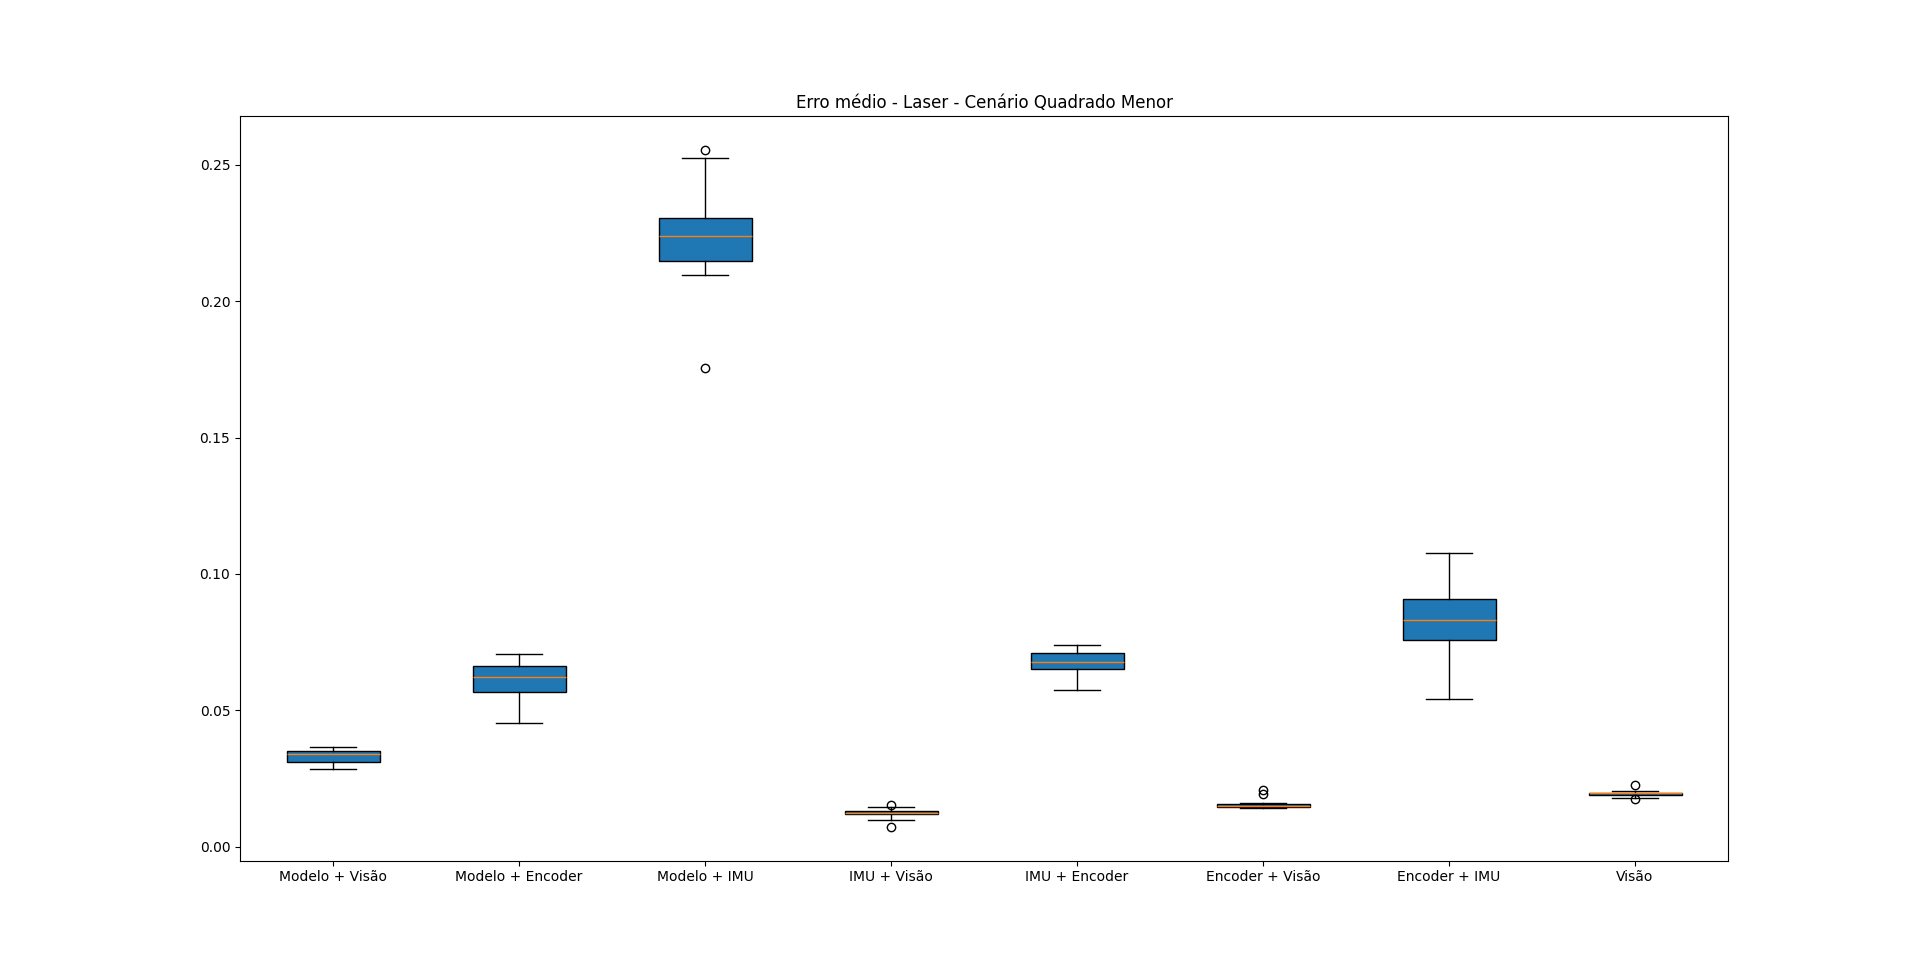
\includegraphics[width=0.9\textwidth]{../Dados/Graficos-Resultados/erro_medio_distancia_quadrado_menor.png}
		\label{fig:erro_medio_distancia_quad_menor}
		\smallcaption{Fonte: o Autor}
	\end{figure}

	Além disso, é possível notar que a utilização de sensores na fase de predição do \glsxtrlong{ekf} traz melhores resultados que a utilização do modelo teórico cinemático do robô omnidirecional da categoria \glsxtrshort{ssl}, visto que as leituras de velocidade e aceleração adquiridas pelos sensores encoder e \glsxtrshort{imu} provém estimativas melhores do que a utilização da velocidade teórica enviada ao robô. Esses resultados podem ser explicados pelas não-linearidades inseridas no movimento de um robô com rodas omnidirecionais, como o atrito, por exemplo.
	
	Sobre os cenários que não utilizam do SSL-Vision, é possível notar que os erros médios desses cenários são maiores que 5cm, sendo o Cenário 3 (modelo + \glsxtrshort{imu}) o pior deles, o que indica um problema na utilização do acelerômetro na fase de correção. Apesar disso, para escopos fora da \glsxtrshort{ssl}, os erros apresentados nos Cenários 2, 5 e 7 são erros considerados aceitáveis, mostrando que eles podem ser usados em cenários em que não é possível a utilização de um sensor que providencia leituras globais de posição, como câmeras e \glsxtrshort{gps}.

	Além disso, também a partir da Figura \ref{fig:erro_medio_distancia_quad_menor}, é possível notar que os cenários que utilizam do sistema global de câmeras da \glsxtrshort{ssl} possuem menos variações em relação ao erro do que os cenários que utilizam apenas os sensores embarcados no robô. Isso demonstra que o erro médio ao longos dos testes nas combinações que utilizam a visão é mais estável do que nas outras combinações.
	
	A Figura \ref{fig:erro_maximo_distancia_quad_menor} mostra a distribuição do erro máximo em metros nos testes do trajeto quadrado menor em cada combinação. O gráfico corrobora com o que foi discutido anteriormente sobre a utilização do sistema global de câmeras na fase de correção do \glsxtrshort{ekf}, em que os cenários que utilizam do SSL-Vision possuem os menores erros máximos ao longo dos trajetos. Além disso, também é possível notar que a utilização dos sensores na fase de predição é superior à utilização do modelo cinemático do robô omnidirecional.
	
	\begin{figure}[!htb]
		\centering
		\caption{Erro máximo no teste com trajeto quadrado menor.}
		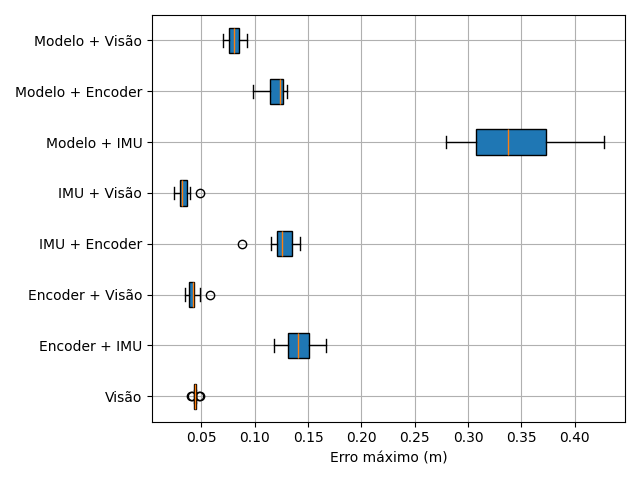
\includegraphics[width=0.9\textwidth]{../Dados/Graficos-Resultados/erro_maximo_distancia_quadrado_menor.png}
		\label{fig:erro_maximo_distancia_quad_menor}
		\smallcaption{Fonte: o Autor}
	\end{figure}

	Apesar do sistema de \textit{ground truth} não ser capaz de capturar a orientação do robô em campo, foi realizada uma comparação das combinações com o próprio sistema de visão com relação à orientação, apenas para título de comparação. Os resultados do erro médio da orientação calculada nos cenários do sistema de fusão de sensores e o que é lido pelo SSL-Vision estão descritos na Figura \ref{fig:erro_medio_orientacao_quad_menor}. 

	\begin{figure}[!htb]
		\centering
		\caption{Erro médio de orientação no teste com trajeto quadrado menor.}
		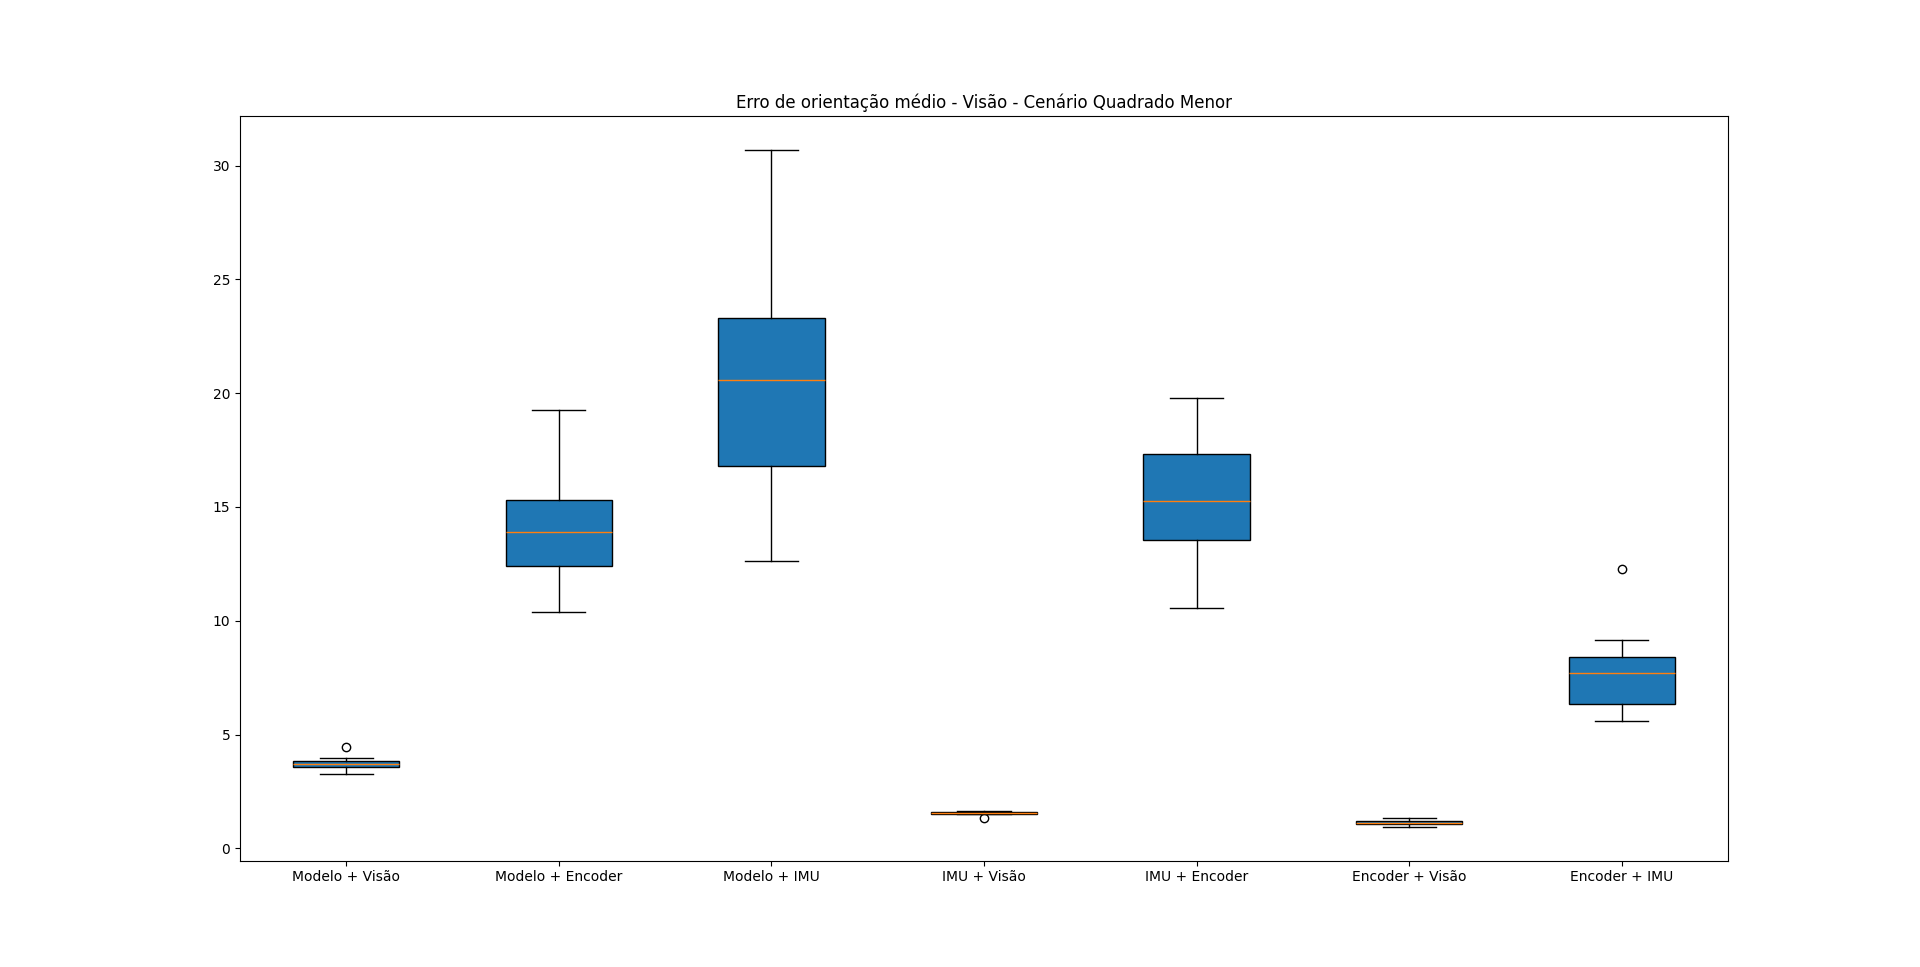
\includegraphics[width=0.9\textwidth]{../Dados/Graficos-Resultados/erro_medio_orientacao_quadrado_menor.png}
		\label{fig:erro_medio_orientacao_quad_menor}
		\smallcaption{Fonte: o Autor}
	\end{figure}

	Assim como na análise do erro médio de distância, é possível analisar que a utilização dos dados do sistema global de câmeras na fase de correção traz melhores resultados do que as combinações que fazem utilização apenas do modelo, encoders ou \glsxtrshort{imu}. Nesses cenários sem o sistema de câmeras, é possível notar que o erro médio é maior do que 5$^\circ$ em todos eles, sendo que, fora o Cenário 7, em todos o erro médio é maior que 10$^\circ$.

	Por fim, a Tabela \ref{tbl:resumo_resultados_quadrado_menor} mostra os resultados gerais obtidos na região de sobreposição de 2 câmeras com relação ao erro médio de distância, erro médio de orientação e o tempo de atualização médio. Quanto ao erro médio de distância é possível analisar que a utilização de sensores, como \glsxtrshort{imu} e encoders (Cenários 4 e 6), consegue resultados levemente superiores comparados com os resultados atingidos pelo sistema atual utilizado pela equipe (Cenário 8), que utiliza somente os dados do sistema de câmeras da liga.

	\begin{table}[!htb]
		\centering
		\caption{Resumo dos resultados obtidos dos cenários no teste do quadrado menor.}
		\label{tbl:resumo_resultados_quadrado_menor}
		\scalebox{0.82}{%
			\begin{tabular}{c|ccc|cc|c}
				\cline{2-6}
				& \multicolumn{3}{c|}{Distância - Erro}                                          & \multicolumn{2}{c|}{Orientação - Erro}               &                              \\ \hline
				\textbf{Cenário}  & \textbf{Média {[}m{]}} & \textbf{Máximo {[}m{]}} & \textbf{Desv. Pad. {[}m{]}} & \textbf{Média {[}deg{]}} & \textbf{Máximo {[}deg{]}} & \textbf{$T_{att}$ {[}ms{]}} \\ \hline
				Modelo + Visão    & 0,033067               & 0,080706                & 0,037178                    & 3,725156                 & 9,467714                  & 3,45970                      \\ \hline
				Modelo + Encoders & 0,060239               & 0,119910                & 0,061663                    & 13,88283                 & 31,08587                  & 3,58013                      \\ \hline
				Modelo + IMU      & 0,223313               & 0,343750                & 0,199025                    & 20,679713                & 57,796915                 & 3,59125                      \\ \hline
				IMU + Visão       & 0,012167               & 0,033837                & 0,014022                    & 1,541681                 & 4,788489                  & 3,51205                      \\ \hline
				IMU + Encoders    & 0,067586               & 0,125119                & 0,061642                    & 15,263899                & 30,86708                  & 3,59578                      \\ \hline
				Encoders + Visão  & 0,015852               & 0,042467                & 0,018073                    & 1,146865                 & 4,148206                  & 3,45462                      \\ \hline
				Encoders + IMU    & 0,083122               & 0,140408                & 0,076724                    & 7,710782                 & 18,938697                 & 3,59147                      \\ \hline
				Visão             & 0,019585               & 0,044054                & 0,018842                    & -                        & -                         & 16,2879                      \\ \hline
			\end{tabular}
		}
	\end{table}

	Além disso, quanto ao tempo de atualização, os resultados obtidos nos cenários com fusão de sensores conseguem um tempo praticamente 5x menor do que o sistema atual da equipe, visto que o \glsxtrshort{ekf} acontece de forma embarcada ao robô, enquanto o sistema atual da equipe depende da taxa de atualização do SSL-Vision.

	\section{Teste com trajeto quadrado maior} \label{sec:resultados_quadrado_maior}
	
		Nesta seção será feita a análise do teste do trajeto quadrado maior em campo. O intuito desse teste é analisar o desempenho das diferentes combinações de sensores propostas para localização do robô numa região do campo em que a distorção da imagem do sistema global de câmeras da \glsxtrshort{ssl} é maior, o que pode levar a maiores erros na detecção da posição do robô em campo.
		
		Na Figura \ref{fig:erro_medio_distancia_quad_maior} é mostrada a distribuição do erro médio de distância nos testes com quadrado maior nos oitos cenários propostos neste projeto. É notável que a utilização dos dados do SSL-Vision leva a erros médios menores comparado com os cenários que não utilizam os dados do sistema de câmeras. Analisando os cenários que não utilizam o SSL-Vision, é possível notar erros médios maiores do que no teste da Seção \ref{sec:resultados_quadrado_menor}, o que mostra que a utilização de um sensor que providencie leituras globais de posição evita erros acumulativos em relação à distância percorrida.
		
		\begin{figure}[!htb]
			\centering
			\caption{Erro médio de distância no teste com trajeto do quadrado maior.}
			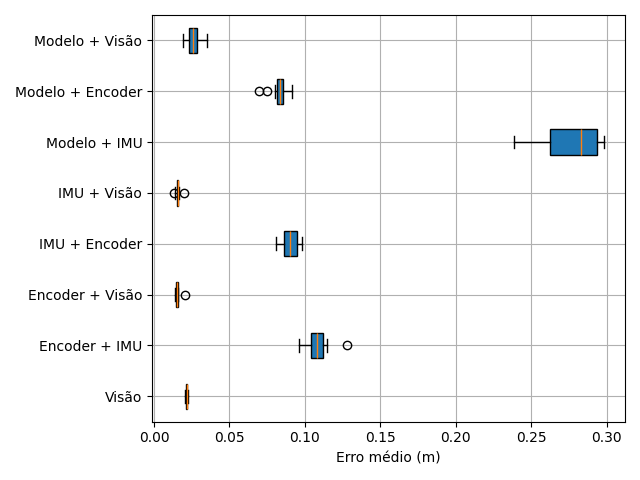
\includegraphics[width=0.9\textwidth]{../Dados/Graficos-Resultados/erro_medio_distancia_quadrado_maior.png}
			\label{fig:erro_medio_distancia_quad_maior}
			\smallcaption{Fonte: o Autor}
		\end{figure}
	
		Assim como nos resultados apresentados quanto ao erro médio nos testes com quadrado menor na Seção \ref{sec:resultados_quadrado_menor}, é possível analisar resultados levemente melhores ao utilizar sensores na fase de predição, como encoders e \glsxtrshort{imu}, junto ao SSL-Vision quando comparado com o sistema atual da equipe que utiliza somente os dados do sistema de visão sem fusão de sensores.
	
		A Figura \ref{fig:erro_maximo_distancia_quad_maior} traz a distribuição dos erros máximos de distância nos cenários analisados. O gráfico corrobora com os resultados do gráfico da Figura \ref{fig:erro_medio_distancia_quad_menor}. É notável também que a utilização do SSL-Vision diminui consideravelmente o erro máximo ao longo do trajeto. Tanto o Cenário 8, que é o sistema atual da equipe, como os cenários que utilizam o SSL-Vision na fase de correção da fusão de sensores, possuem erro máximo menor que 5cm, que representa menos que 1/3 do tamanho máximo de um robô típico da categoria \glsxtrshort{ssl}. % O gráfico corrobora com o que foi trazido anteriormente de a pior combinação ser a do Cenário 3 (Modelo + \glsxtrshort{imu}), com erro máximo entre 35cm e 45cm nos testes realizados, o que representa uma distância de 2 a 2,5 vezes o tamanho de um robô típico da categoria \glsxtrshort{ssl}.
		
		\begin{figure}[!htb]
			\centering
			\caption{Erro máximo no teste com trajeto do quadrado maior.}
			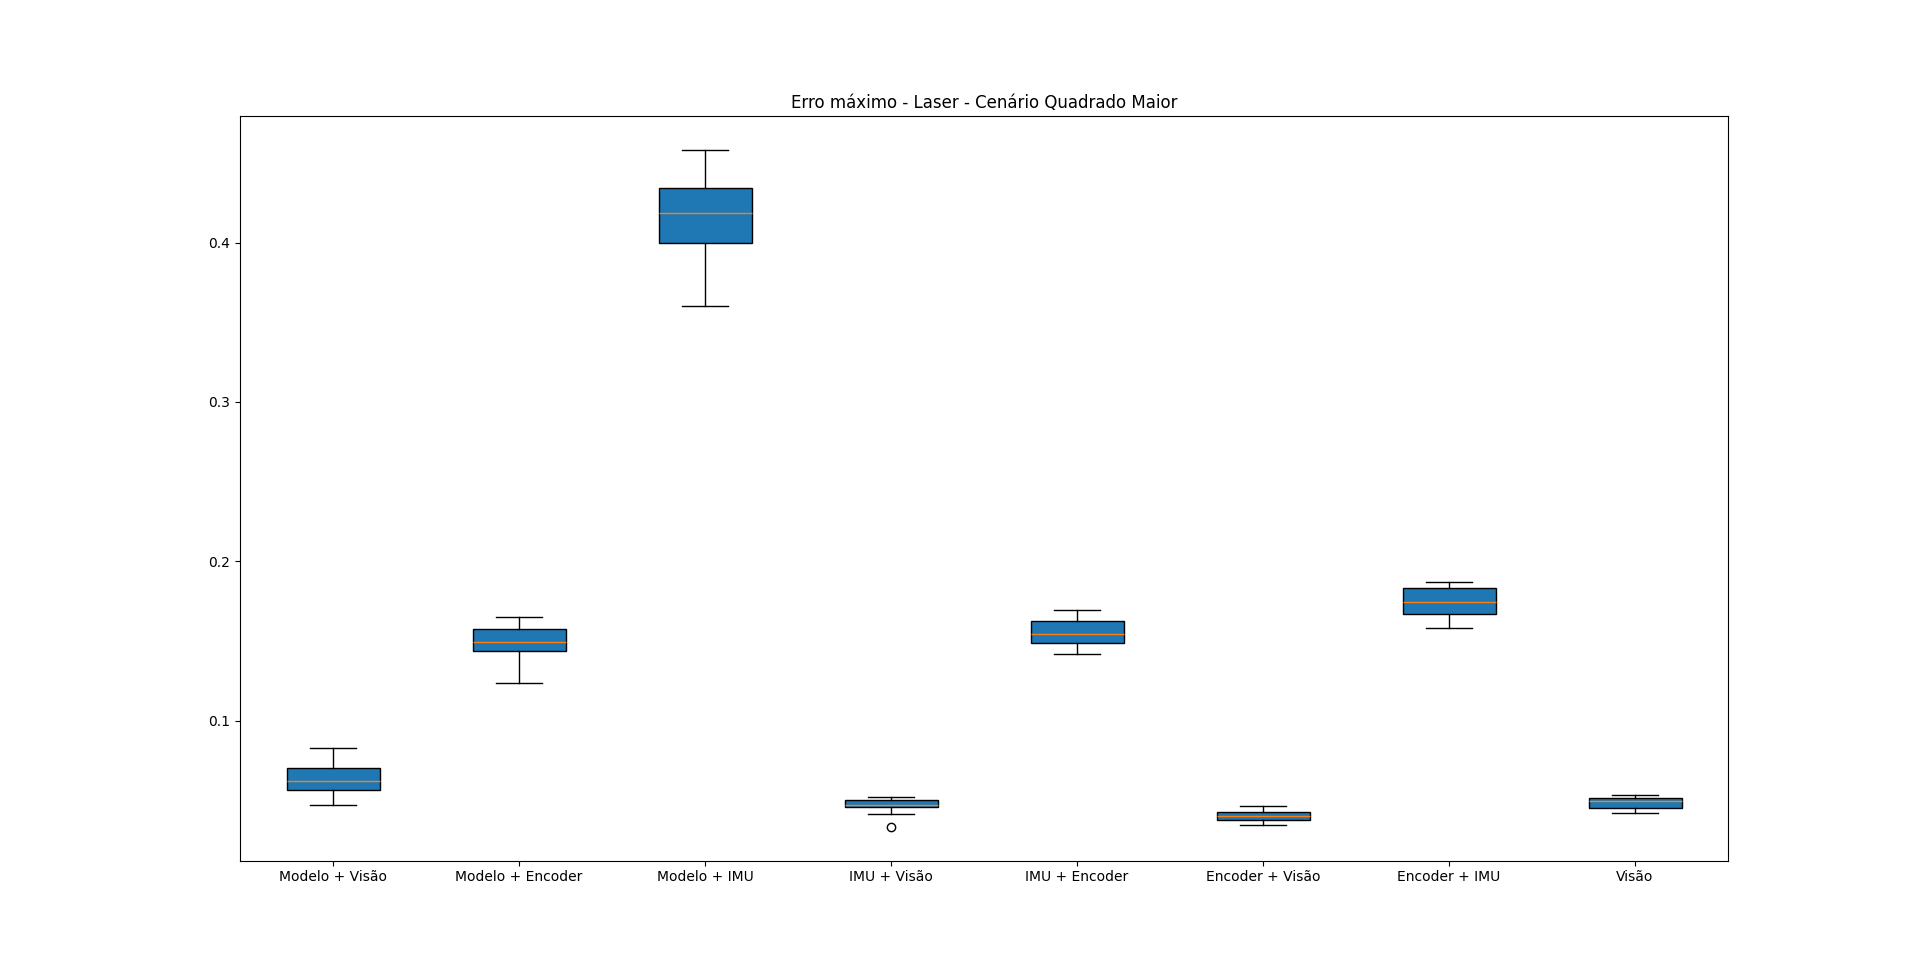
\includegraphics[width=0.9\textwidth]{../Dados/Graficos-Resultados/erro_maximo_distancia_quadrado_maior.png}
			\label{fig:erro_maximo_distancia_quad_maior}
			\smallcaption{Fonte: o Autor}
		\end{figure}
	
		A Figura \ref{fig:erro_medio_orientacao_quad_maior} traz a média do erro de orientação em relação ao sistema de visão quanto a orientação somente a título de comparação. Assim como na análise quanto ao erro de distância, a utilização do SSL-Vision na fase de correção traz resultados melhores quanto a uniformidade e média. Apesar disso, é possível notar que o Cenário 7 traz resultados aceitáveis quanto a orientação (menor que 10$^\circ$), mostrando que a utilização do encoder na fase de predição é melhor do que na fase de correção, o que pode ser explicado pela integração direta da velocidade angular calculada a partir das leituras dos encoders nas rodas, o que aumenta o erro acumulado, diferente do que acontece na fase de predição, que a estimativa da orientação leva em conta o estado passado do \glsxtrshort{ekf}.
	
		\begin{figure}[!htb]
			\centering
			\caption{Erro médio de orientação no teste com trajeto do quadrado maior.}
			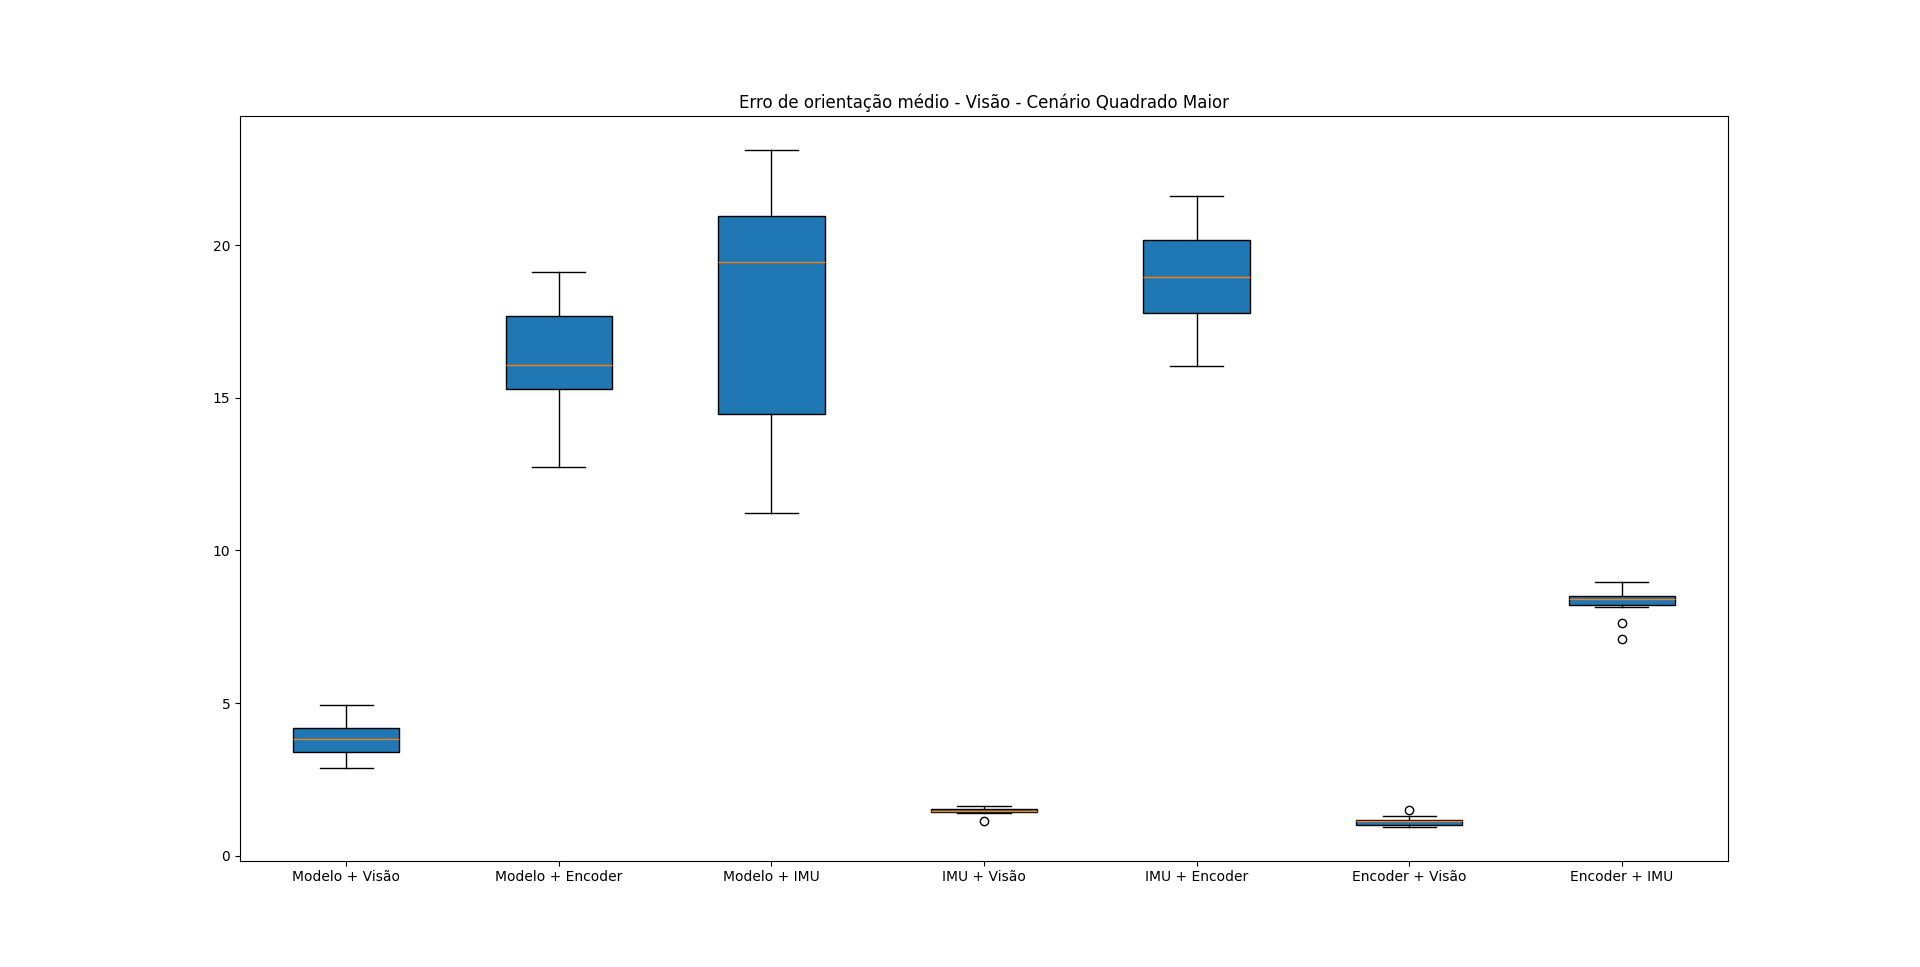
\includegraphics[width=0.9\textwidth]{../Dados/Graficos-Resultados/erro_medio_orientacao_quadrado_maior.png}
			\label{fig:erro_medio_orientacao_quad_maior}
			\smallcaption{Fonte: o Autor}
		\end{figure}
	
		A Figura \ref{fig:orientacao_imu_encoder} mostra como a orientação calculada pelo \glsxtrshort{ekf} começa a desviar do que é lido pelo SSL-Vision no Cenário 5 (\glsxtrshort{imu} + encoders), mostrando um acúmulo de erro ao longo do trajeto. Já na Figura \ref{fig:orientacao_encoder_imu}, que mostra a orientação calculada pelo \glsxtrshort{ekf} no Cenário 7 (encoders + \glsxtrshort{imu}), não é notável esse acúmulo ao longo do tempo, mesmo que os sensores utilizados sejam os mesmos.
	
		\begin{figure}
			\centering
			\begin{minipage}[t]{0.47\textwidth}
				\centering
				\caption{Orientação ao longo de uma amostra do Cenário 5.}
				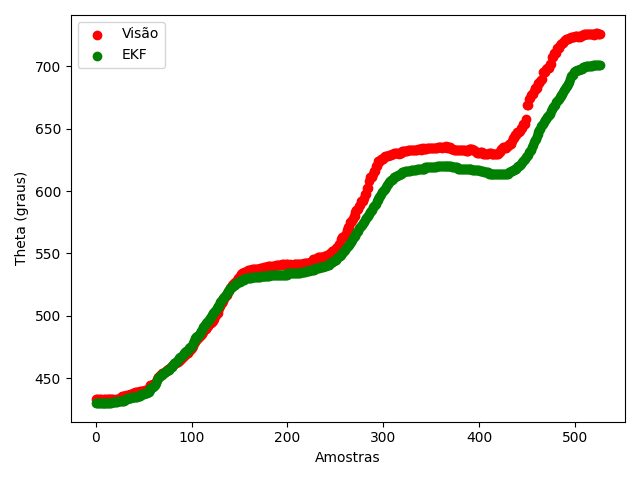
\includegraphics[width=\textwidth]{orientacao_imu_encoder.png}
				\label{fig:orientacao_imu_encoder}
				\smallcaption{Fonte: o Autor}
			\end{minipage}
			\hspace{1em}
			\begin{minipage}[t]{0.47\textwidth}
				\centering
				\caption{Orientação ao longo de uma amostra do Cenário 7.}
				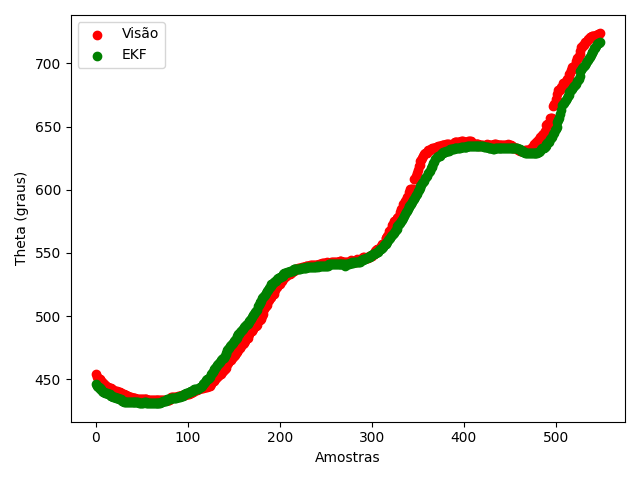
\includegraphics[width=\textwidth]{orientacao_encoder_imu.png}
				\label{fig:orientacao_encoder_imu}
				\smallcaption{Fonte: o Autor}
			\end{minipage}
		\end{figure}
	
		Por fim, a Tabela \ref{tbl:resumo_resultados_quadrado_maior} traz os resultados gerais obtidos na região de maior distorção por conta do efeito olho de peixe das câmeras com relação ao erro médio de distancia, erro médio de orientação e o tempo de atualização médio. Quanto à posição, assim como no trajeto quadrado menor, os cenários que utilizam sensores na fase de predição (Cenários 4 e 6) junto do SSL-Vision na fase de correção apresentam resultados levemente melhores do que o sistema atual da equipe (Cenário 8) em relação à média, valor máximo e desvio padrão.
		
		Quanto ao tempo de atualização da estimativa de posição, os resultados obtidos também seguem o que foi observado na Seção \ref{sec:resultados_quadrado_menor}, em que o sistema atual utilizado pela equipe RoboFEI tem média praticamente 5 vezes superior aos cenários de fusão de sensores de forma embarcada. Esse resultado obtido com a fusão de sensores é essencial para um bom controle de posição, como descrito na Seção \ref{sec:fusao_sensores_ssl}.
	
		\begin{table}[!htb]
			\centering
			\caption{Resumo dos resultados obtidos dos cenários no teste com quadrado maior.}
			\label{tbl:resumo_resultados_quadrado_maior}
			\scalebox{0.82}{%
				\begin{tabular}{c|ccc|cc|c}
					\cline{2-6}
					& \multicolumn{3}{c|}{Distância - Erro}                                          & \multicolumn{2}{c|}{Orientação - Erro}               &                              \\ \hline
					\textbf{Cenário}  & \textbf{Média {[}m{]}} & \textbf{Máximo {[}m{]}} & \textbf{Desv. Pad. {[}m{]}} & \textbf{Média {[}deg{]}} & \textbf{Máximo {[}deg{]}} & \textbf{$T_{att}$ {[}ms{]}} \\ \hline
					Modelo + Visão    & 0,02586                & 0,062953                & 0,028476                    & 3,824521                 & 15,458832                 & 3,47707                      \\ \hline
					Modelo + Encoders & 0,082803               & 0,149021                & 0,073858                    & 16,23678                 & 38,790607                 & 3,58073                      \\ \hline
					Modelo + IMU      & 0,277591               & 0,413911                & 0,222238                    & 17,841146                & 45,34764                  & 3,59174                      \\ \hline
					IMU + Visão       & 0,015806               & 0,046374                & 0,019426                    & 1,470293                 & 5,637516                  & 3,52665                      \\ \hline
					IMU + Encoders    & 0,089906               & 0,155431                & 0,07952                     & 18,94846                 & 46,190327                 & 3,59629                      \\ \hline
					Encoders + Visão  & 0,015518               & 0,040223                & 0,01688                     & 1,128545                 & 3,986355                  & 3,46823                      \\ \hline
					Encoders + IMU    & 0,108431               & 0,174239                & 0,093185                    & 8,268624                 & 23,724647                 & 3,59208                      \\ \hline
					Visão             & 0,021699               & 0,048287                & 0,020637                    & -                        & -                         & 16,4081                      \\ \hline
				\end{tabular}
			}
		\end{table}

	\section{Considerações finais}
	
		A partir do que foi analisado com os gráficos em cada um dos trajetos propostos para análise dos resultados, é possível notar que a utilização de um sensor que te dê informações absolutas do seu robô em relação ao ambiente é essencial para a fusão de sensores. Especialmente na \glsxtrshort{ssl}, que a precisão necessária para realização de jogadas é alta por conta da velocidade e tamanho tanto dos robôs, quanto da bola utilizada, utilizar o sistema de visão da liga é essencial para realizar a fusão de sensores para localização de forma embarcada.
		
		Entretanto, é notável que a fusão de sensores é superior à utilização sozinha dos dados do sistema de visão, tanto por conta da leve melhoria e confiabilidade alcançada ao utilizar outros sensores junto ao SSL-Vision, quanto pelo tempo de atualização praticamente 5 vezes mais demorado do que o sistema de fusão de sensores. Como mostrado na Seção \ref{sec:fusao_sensores_ssl}, um sistema de localização embarcado é essencial para realização de jogadas na \glsxtrshort{ssl} ao tornar viável a mudança do controle de posição dos robôs para seu microcontrolador ao invés do computador central utilizado pelas equipes.
		
		A partir do que foi analisado nos resultados obtidos nos testes em diferentes regiões do campo, descrito nas Seções \ref{sec:resultados_quadrado_menor} e \ref{sec:resultados_quadrado_maior}, é notável que as melhores combinações foram nos Cenários 4 e 6, que utilizam os sensores \glsxtrshort{imu} e encoders, respectivamente, junto aos dados do SSL-Vision para a fusão de sensores.
		
		Um efeito que acontece durante partidas da \glsxtrshort{ssl} é a oclusão, seja da bolinha ou dos robôs, muito por conta de a iluminação não ser uniforme comparando diferentes regiões do campo. Essas situações acontecem em sua maioria nas regiões perto do escanteio, ou próxima aos gols no campo, e durante curtos períodos de tempo normalmente (de 1 a 2 segundos, como piscadas), visto a dinâmica das partidas. Sabendo disso, decidiu-se testar as duas melhores combinações em situações até mais críticas do que essa descrita, no caso com o robô não sendo notado pelo sistema de visão durante 8 segundos no trajeto.
		
		As Figuras \ref{fig:teste_imu_8s} e \ref{fig:teste_encoder_8s} mostram os testes realizados desconsiderando os dados do SSL-Vision durante 8 segundos de trajeto para os Cenários 4 e 6, respectivamente. No caso, os pontos em vermelho são as posições calculadas pelo \glsxtrshort{ekf} que utilizam os dados do SSL-Vision para correção, enquanto os pontos em azul são os pontos que o sistema para de considerar os dados do SSL-Vision, performando apenas a fase de predição, já os pontos em preto são os pontos do sistema de \textit{ground truth}.
		
		\begin{figure}[!htb]
			\centering
			\caption{Teste de 8 segundos sem visão para o Cenário 4.}
			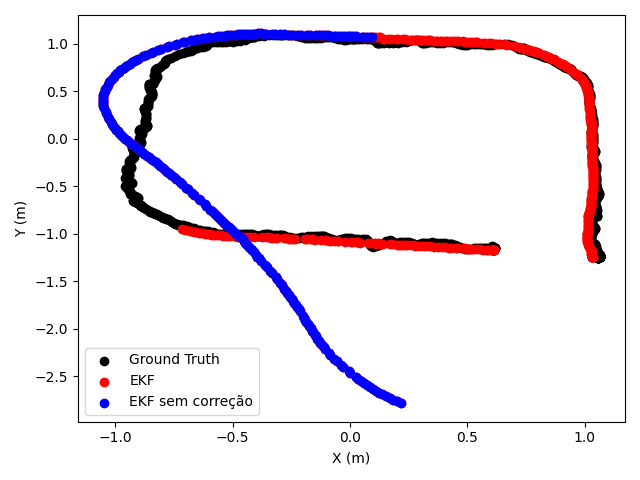
\includegraphics[width=0.8\textwidth]{teste_imu_8s.png}
			\label{fig:teste_imu_8s}
			\smallcaption{Fonte: o Autor}
		\end{figure}
		
		\begin{figure}[!htb]
			\centering
			\caption{Teste de 8 segundos sem visão para o Cenário 6.}
			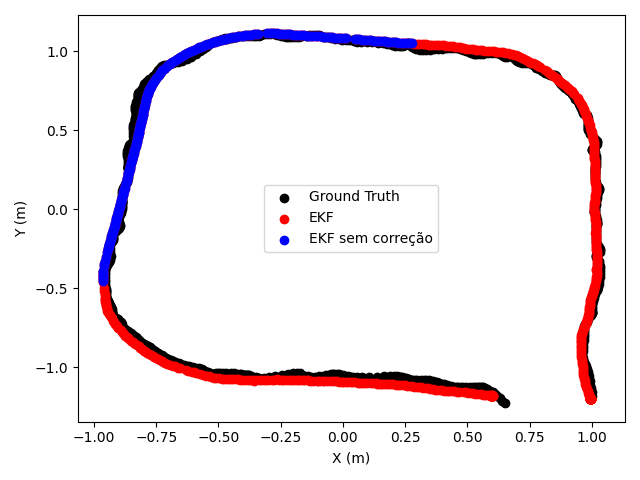
\includegraphics[width=0.8\textwidth]{teste_encoder_8s.png}
			\label{fig:teste_encoder_8s}
			\smallcaption{Fonte: o Autor}
		\end{figure}
	
		É notável que a \glsxtrshort{imu} consegue predizer bem a posição do robô até 2 segundos. Porém, após esse tempo, por conta da integração dos valores de aceleração para obter dados de posição e velocidade, começa a aumentar significativamente o erro, e volta para o trajeto quando os dados da visão retornam. Enquanto isso, os encoders conseguem predizer bem a localização do robô durante esse tempo expressivo sem os dados do sistema de visão global, já que a maior causa de erros para as leituras do encoder é em momentos de aceleração ou desaceleração do robô por conta de derrapagens, o que pode ser evitado com os dados do acelerômetro, por exemplo.
		
		A partir dos testes sem o sistema de visão durante 8 segundos e dos resultados descritos nas Seções \ref{sec:resultados_quadrado_menor} e \ref{sec:resultados_quadrado_maior}, é possível colocar que a utilização do encoder seja mais benéfica do que a utilização da \glsxtrshort{imu}, visto que os resultados de ambas são parecidos quando há informação disponível do SSL-Vision, mas sem o sistema de visão há um erro acumulado grande em pouco tempo utilizando a \glsxtrshort{imu} somente. 
		
		Considerando que o sistema está inserido dentro do ambiente da \acrshort{ssl}, uma solução também seria, enquanto uma nova informação do SSL-Vision não estiver disponível, realizar a fusão dos encoders e \acrshort{imu} para suprimir os pontos fracos de cada um. No caso, os dados dos encoders impediriam o aumento da incerteza dos estados do \acrshort{ekf} em situações que o robô esteja parado por conta do erro acumulado da \acrshort{imu}, enquanto a \acrshort{imu} atuaria bem em situações de derrapagem durante acelerações do robô.
		
%		Considerando que o sistema está inserido na lógica do \glsxtrshort{ssl}, o sistema de localização da equipe pode ser desenvolvido para lidar com as situações que o robô não é identificado pelo sistema de visão, como realizar a fusão entre encoder e \glsxtrshort{imu} após um determinado tempo que o robô não seja identificado. Assim, os dados dos encoders evitariam o aumento de incerteza dos estados do \glsxtrshort{ekf}, diferente da utilização da \acrshort{imu}, que acumularia um erro em pouco tempo, mesmo que o robô esteja parado.
		
		Fora do ambiente da \acrshort{ssl}, caso não haja a possibilidade de utilização de um sensor que forneça informações globais, como LiDAR, câmera ou GPS, apenas a utilização de \glsxtrshort{imu} e encoder pode trazer resultados aceitáveis (abaixo de 10cm na média de um trajeto), ou até a utilização do modelo sendo corrigido pelos dados do encoder (Cenário 2). Porém, os resultados mostram que a utilização de um sensor global traz uma ótima precisão para um projeto de localização de um robô móvel.

\chapter{Conclusão} \label{sec:conclusao}

	Este trabalho realizou uma análise comparativa do uso de diferentes sensores num sistema de localização baseado em fusão de sensores de forma embarcada aplicado no ambiente da categoria \glsxtrshort{ssl} de futebol de robôs da RoboCup. Para realizar a fusão dos diferentes sensores foi escolhido utilizar um \glsxtrlong{ekf}, que é separado nas fases de predição e correção. Os sensores escolhidos foram os seguintes: encoders acoplados às rodas do robô, giroscópio e acelerômetro presentes na placa eletrônica do robô para medições de velocidade angular e aceleração linear, respectivamente, o sistema de câmeras da categoria \glsxtrshort{ssl} e, por fim, o modelo cinemático de um robô omnidirecional de 4 rodas.
	
	Além da implementação do sistema de fusão de sensores, o sistema de \textit{ground truth} também foi desenvolvido para esse projeto e é baseado nas leituras de dois LiDARs, cada um posicionado em um dos gols do campo. O sistema utiliza \glsxtrlong{ht} para identificação de um padrão circular na imagem dos pontos dos LiDARs. Os resultados obtidos mostraram a qualidade do sistema com erro médio próximo de 0,5cm em ambos os eixos do campo, apesar do sistema ser menos uniforme ao apresentar um desvio padrão maior que o sistema de câmeras da \glsxtrshort{ssl}.
	
	Através do erro médio em relação ao sistema de \textit{ground truth} e o tempo de atualização da estimativa de localização foi possível analisar de maneira aprofundada o desempenho dos sensores escolhidos em trajetos distintos para um sistema de localização de forma embarcada.
	
	Os dois testes conduzidos visaram analisar as combinações propostas de fusão de sensores em situações características do sistema de câmeras, que no caso são a região de sobreposição de câmeras, normalmente situada no centro do campo e que leva a divergências na posição observada dos robôs por duplicações, e na região de distorção das câmeras, que normalmente acontece nas bordas do campo por conta do efeito olho de peixe das lentes utilizadas e acaba influenciando na posição lida pelo sistema.
	
	Os resultados obtidos demonstraram que as melhores combinações para os robôs da categoria \glsxtrshort{ssl} utilizam os dados de sensores na fase de predição do \glsxtrshort{ekf} e o SSL-Vision na fase de correção, apesar das deficiências demonstradas do sistema. Isso é notável analisando o erro médio em relação ao sistema de \textit{ground truth}, assim como os valores máximos e os desvios padrões, dos Cenários 4 e 6 comparados com os outros. Os dados dos sensores provém melhores estimativas de velocidade e aceleração durante a movimentação do robô. Já a utilização do modelo cinemático do robô omnidirecional na fase de predição não se provou uma boa opção, justificado por não levar em conta o atrito das rodas omnidirecionais, por exemplo, ou até mesmo não-linearidades envolvidas no movimento do robô.
	
	Embora o SSL-Vision forneça a pose do robô a uma taxa de 60 frames por segundo aproximadamente, é importante que no intervalo entre frames o robô mantenha estimativas da sua posição devido a dinamicidade das partidas da \acrshort{ssl} a fim de realizar chutes ou interceptações mais precisas. Portanto, um sistema de localização embarcado com um período de atualização em torno de 3.5ms é ideal para a realização de jogadas durantes as partidas, como as combinações de fusão de sensores testadas nesse projeto.
	
	Apesar de os testes estarem inseridos na lógica do futebol de robôs, especialmente na categoria \glsxtrshort{ssl}, os resultados obtidos nesse estudo podem beneficiar outras aplicações de robótica móvel, como robôs de serviço ou robôs humanoides. Por exemplo, apesar de os resultados obtidos nos cenários que não utilizam o sistema global de visão da liga não serem satisfatórios para a aplicação, acredita-se que os erros calculados sejam aceitáveis em aplicações de robôs maiores e mais robustos, e que até fazem utilização de outros sensores globais, como LiDARs em aplicações internas ou \glsxtrshort{gps} em aplicações externas.
	
	Trabalhos futuros relacionados estão ligados à implementação do sistema de localização de fusão de sensores testado nesse trabalho em um controle de posição dos robôs da categoria de modo embarcado, mostrando a efetividade do sistema de localização na malha de controle do robô a fim de melhorar a jogabilidade da equipe em campeonatos.
	
\printbibliography

\anexos

\chapter{Artigo publicado no simpósio CROS 2025}

%\setlength{\voffset}{0cm}
%\setlength{\hoffset}{0cm}
%
%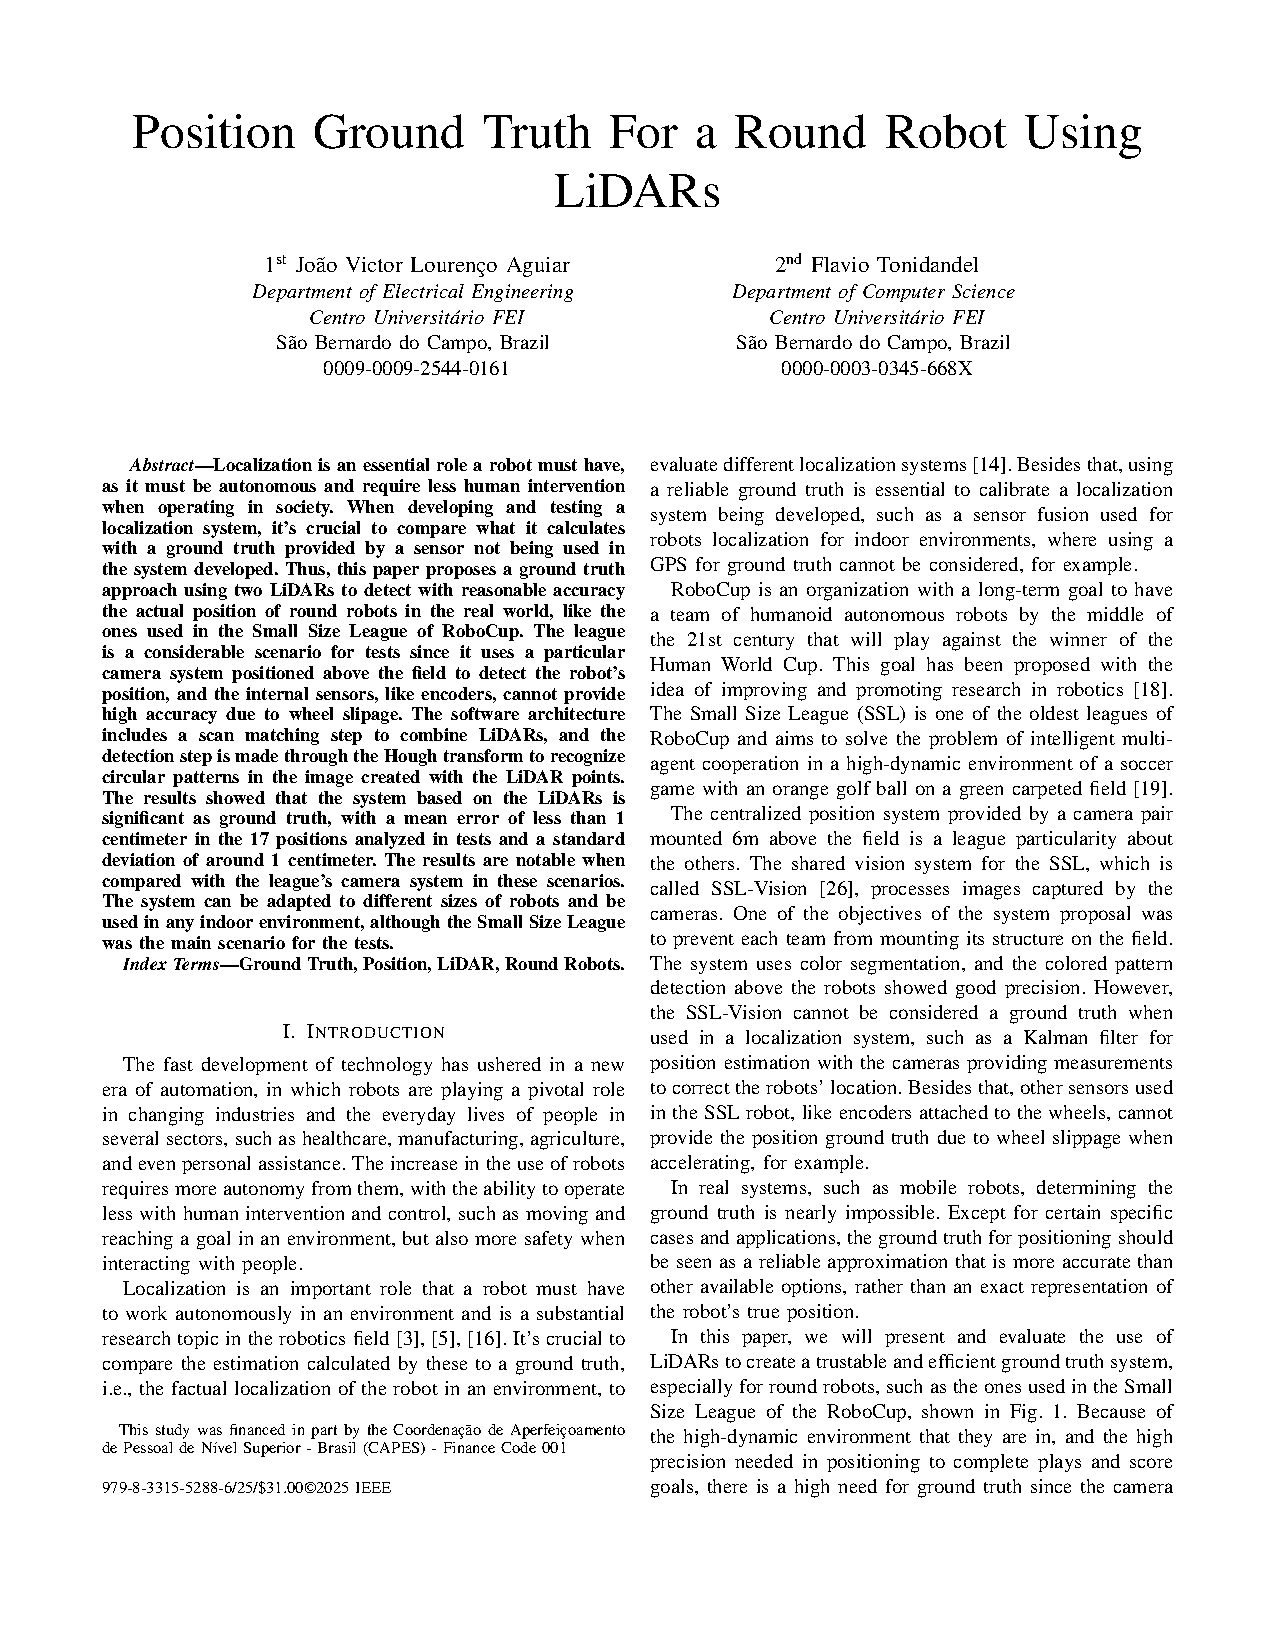
\includepdf[pages=-, pagecommand={},width=\textwidth]{groundtruthlidar.pdf}
\includepdf[pages=-]{groundtruthlidar.pdf}
%
%\setlength{\voffset}{-2.54cm}
%\setlength{\hoffset}{-2.54cm}

%\clearpage
%\thispagestyle{empty}  % remove cabeçalho e rodapé
%\noindent   
%\begin{figure}[p]
%	\centering
%	\includegraphics[width=\paperwidth,height=\paperheight,keepaspectratio, page={1}]{groundtruthlidar.pdf}
%\end{figure}
%\clearpage
%\includegraphics[scale=1.00,page={2}]{groundtruthlidar.pdf}

\end{document}